% Options for packages loaded elsewhere
\PassOptionsToPackage{unicode}{hyperref}
\PassOptionsToPackage{hyphens}{url}
\PassOptionsToPackage{dvipsnames,svgnames,x11names}{xcolor}
%
\documentclass[
  letterpaper,
  DIV=11,
  numbers=noendperiod]{scrartcl}

\usepackage{amsmath,amssymb}
\usepackage{iftex}
\ifPDFTeX
  \usepackage[T1]{fontenc}
  \usepackage[utf8]{inputenc}
  \usepackage{textcomp} % provide euro and other symbols
\else % if luatex or xetex
  \usepackage{unicode-math}
  \defaultfontfeatures{Scale=MatchLowercase}
  \defaultfontfeatures[\rmfamily]{Ligatures=TeX,Scale=1}
\fi
\usepackage{lmodern}
\ifPDFTeX\else  
    % xetex/luatex font selection
\fi
% Use upquote if available, for straight quotes in verbatim environments
\IfFileExists{upquote.sty}{\usepackage{upquote}}{}
\IfFileExists{microtype.sty}{% use microtype if available
  \usepackage[]{microtype}
  \UseMicrotypeSet[protrusion]{basicmath} % disable protrusion for tt fonts
}{}
\makeatletter
\@ifundefined{KOMAClassName}{% if non-KOMA class
  \IfFileExists{parskip.sty}{%
    \usepackage{parskip}
  }{% else
    \setlength{\parindent}{0pt}
    \setlength{\parskip}{6pt plus 2pt minus 1pt}}
}{% if KOMA class
  \KOMAoptions{parskip=half}}
\makeatother
\usepackage{xcolor}
\ifLuaTeX
  \usepackage{luacolor}
  \usepackage[soul]{lua-ul}
\else
  \usepackage{soul}
  
\fi
\setlength{\emergencystretch}{3em} % prevent overfull lines
\setcounter{secnumdepth}{5}
% Make \paragraph and \subparagraph free-standing
\makeatletter
\ifx\paragraph\undefined\else
  \let\oldparagraph\paragraph
  \renewcommand{\paragraph}{
    \@ifstar
      \xxxParagraphStar
      \xxxParagraphNoStar
  }
  \newcommand{\xxxParagraphStar}[1]{\oldparagraph*{#1}\mbox{}}
  \newcommand{\xxxParagraphNoStar}[1]{\oldparagraph{#1}\mbox{}}
\fi
\ifx\subparagraph\undefined\else
  \let\oldsubparagraph\subparagraph
  \renewcommand{\subparagraph}{
    \@ifstar
      \xxxSubParagraphStar
      \xxxSubParagraphNoStar
  }
  \newcommand{\xxxSubParagraphStar}[1]{\oldsubparagraph*{#1}\mbox{}}
  \newcommand{\xxxSubParagraphNoStar}[1]{\oldsubparagraph{#1}\mbox{}}
\fi
\makeatother

\usepackage{color}
\usepackage{fancyvrb}
\newcommand{\VerbBar}{|}
\newcommand{\VERB}{\Verb[commandchars=\\\{\}]}
\DefineVerbatimEnvironment{Highlighting}{Verbatim}{commandchars=\\\{\}}
% Add ',fontsize=\small' for more characters per line
\usepackage{framed}
\definecolor{shadecolor}{RGB}{241,243,245}
\newenvironment{Shaded}{\begin{snugshade}}{\end{snugshade}}
\newcommand{\AlertTok}[1]{\textcolor[rgb]{0.68,0.00,0.00}{#1}}
\newcommand{\AnnotationTok}[1]{\textcolor[rgb]{0.37,0.37,0.37}{#1}}
\newcommand{\AttributeTok}[1]{\textcolor[rgb]{0.40,0.45,0.13}{#1}}
\newcommand{\BaseNTok}[1]{\textcolor[rgb]{0.68,0.00,0.00}{#1}}
\newcommand{\BuiltInTok}[1]{\textcolor[rgb]{0.00,0.23,0.31}{#1}}
\newcommand{\CharTok}[1]{\textcolor[rgb]{0.13,0.47,0.30}{#1}}
\newcommand{\CommentTok}[1]{\textcolor[rgb]{0.37,0.37,0.37}{#1}}
\newcommand{\CommentVarTok}[1]{\textcolor[rgb]{0.37,0.37,0.37}{\textit{#1}}}
\newcommand{\ConstantTok}[1]{\textcolor[rgb]{0.56,0.35,0.01}{#1}}
\newcommand{\ControlFlowTok}[1]{\textcolor[rgb]{0.00,0.23,0.31}{\textbf{#1}}}
\newcommand{\DataTypeTok}[1]{\textcolor[rgb]{0.68,0.00,0.00}{#1}}
\newcommand{\DecValTok}[1]{\textcolor[rgb]{0.68,0.00,0.00}{#1}}
\newcommand{\DocumentationTok}[1]{\textcolor[rgb]{0.37,0.37,0.37}{\textit{#1}}}
\newcommand{\ErrorTok}[1]{\textcolor[rgb]{0.68,0.00,0.00}{#1}}
\newcommand{\ExtensionTok}[1]{\textcolor[rgb]{0.00,0.23,0.31}{#1}}
\newcommand{\FloatTok}[1]{\textcolor[rgb]{0.68,0.00,0.00}{#1}}
\newcommand{\FunctionTok}[1]{\textcolor[rgb]{0.28,0.35,0.67}{#1}}
\newcommand{\ImportTok}[1]{\textcolor[rgb]{0.00,0.46,0.62}{#1}}
\newcommand{\InformationTok}[1]{\textcolor[rgb]{0.37,0.37,0.37}{#1}}
\newcommand{\KeywordTok}[1]{\textcolor[rgb]{0.00,0.23,0.31}{\textbf{#1}}}
\newcommand{\NormalTok}[1]{\textcolor[rgb]{0.00,0.23,0.31}{#1}}
\newcommand{\OperatorTok}[1]{\textcolor[rgb]{0.37,0.37,0.37}{#1}}
\newcommand{\OtherTok}[1]{\textcolor[rgb]{0.00,0.23,0.31}{#1}}
\newcommand{\PreprocessorTok}[1]{\textcolor[rgb]{0.68,0.00,0.00}{#1}}
\newcommand{\RegionMarkerTok}[1]{\textcolor[rgb]{0.00,0.23,0.31}{#1}}
\newcommand{\SpecialCharTok}[1]{\textcolor[rgb]{0.37,0.37,0.37}{#1}}
\newcommand{\SpecialStringTok}[1]{\textcolor[rgb]{0.13,0.47,0.30}{#1}}
\newcommand{\StringTok}[1]{\textcolor[rgb]{0.13,0.47,0.30}{#1}}
\newcommand{\VariableTok}[1]{\textcolor[rgb]{0.07,0.07,0.07}{#1}}
\newcommand{\VerbatimStringTok}[1]{\textcolor[rgb]{0.13,0.47,0.30}{#1}}
\newcommand{\WarningTok}[1]{\textcolor[rgb]{0.37,0.37,0.37}{\textit{#1}}}

\providecommand{\tightlist}{%
  \setlength{\itemsep}{0pt}\setlength{\parskip}{0pt}}\usepackage{longtable,booktabs,array}
\usepackage{calc} % for calculating minipage widths
% Correct order of tables after \paragraph or \subparagraph
\usepackage{etoolbox}
\makeatletter
\patchcmd\longtable{\par}{\if@noskipsec\mbox{}\fi\par}{}{}
\makeatother
% Allow footnotes in longtable head/foot
\IfFileExists{footnotehyper.sty}{\usepackage{footnotehyper}}{\usepackage{footnote}}
\makesavenoteenv{longtable}
\usepackage{graphicx}
\makeatletter
\newsavebox\pandoc@box
\newcommand*\pandocbounded[1]{% scales image to fit in text height/width
  \sbox\pandoc@box{#1}%
  \Gscale@div\@tempa{\textheight}{\dimexpr\ht\pandoc@box+\dp\pandoc@box\relax}%
  \Gscale@div\@tempb{\linewidth}{\wd\pandoc@box}%
  \ifdim\@tempb\p@<\@tempa\p@\let\@tempa\@tempb\fi% select the smaller of both
  \ifdim\@tempa\p@<\p@\scalebox{\@tempa}{\usebox\pandoc@box}%
  \else\usebox{\pandoc@box}%
  \fi%
}
% Set default figure placement to htbp
\def\fps@figure{htbp}
\makeatother
% definitions for citeproc citations
\NewDocumentCommand\citeproctext{}{}
\NewDocumentCommand\citeproc{mm}{%
  \begingroup\def\citeproctext{#2}\cite{#1}\endgroup}
\makeatletter
 % allow citations to break across lines
 \let\@cite@ofmt\@firstofone
 % avoid brackets around text for \cite:
 \def\@biblabel#1{}
 \def\@cite#1#2{{#1\if@tempswa , #2\fi}}
\makeatother
\newlength{\cslhangindent}
\setlength{\cslhangindent}{1.5em}
\newlength{\csllabelwidth}
\setlength{\csllabelwidth}{3em}
\newenvironment{CSLReferences}[2] % #1 hanging-indent, #2 entry-spacing
 {\begin{list}{}{%
  \setlength{\itemindent}{0pt}
  \setlength{\leftmargin}{0pt}
  \setlength{\parsep}{0pt}
  % turn on hanging indent if param 1 is 1
  \ifodd #1
   \setlength{\leftmargin}{\cslhangindent}
   \setlength{\itemindent}{-1\cslhangindent}
  \fi
  % set entry spacing
  \setlength{\itemsep}{#2\baselineskip}}}
 {\end{list}}
\usepackage{calc}
\newcommand{\CSLBlock}[1]{\hfill\break\parbox[t]{\linewidth}{\strut\ignorespaces#1\strut}}
\newcommand{\CSLLeftMargin}[1]{\parbox[t]{\csllabelwidth}{\strut#1\strut}}
\newcommand{\CSLRightInline}[1]{\parbox[t]{\linewidth - \csllabelwidth}{\strut#1\strut}}
\newcommand{\CSLIndent}[1]{\hspace{\cslhangindent}#1}

\usepackage{booktabs}
\usepackage{caption}
\usepackage{longtable}
\usepackage{colortbl}
\usepackage{array}
\usepackage{anyfontsize}
\usepackage{multirow}
\usepackage{fvextra}
\DefineVerbatimEnvironment{Highlighting}{Verbatim}{breaklines,commandchars=\\\{\}}
\DefineVerbatimEnvironment{OutputCode}{Verbatim}{breaklines,commandchars=\\\{\}}
\KOMAoption{captions}{tableheading}
\makeatletter
\@ifpackageloaded{caption}{}{\usepackage{caption}}
\AtBeginDocument{%
\ifdefined\contentsname
  \renewcommand*\contentsname{Table of contents}
\else
  \newcommand\contentsname{Table of contents}
\fi
\ifdefined\listfigurename
  \renewcommand*\listfigurename{List of Figures}
\else
  \newcommand\listfigurename{List of Figures}
\fi
\ifdefined\listtablename
  \renewcommand*\listtablename{List of Tables}
\else
  \newcommand\listtablename{List of Tables}
\fi
\ifdefined\figurename
  \renewcommand*\figurename{Figure}
\else
  \newcommand\figurename{Figure}
\fi
\ifdefined\tablename
  \renewcommand*\tablename{Table}
\else
  \newcommand\tablename{Table}
\fi
}
\@ifpackageloaded{float}{}{\usepackage{float}}
\floatstyle{ruled}
\@ifundefined{c@chapter}{\newfloat{codelisting}{h}{lop}}{\newfloat{codelisting}{h}{lop}[chapter]}
\floatname{codelisting}{Listing}
\newcommand*\listoflistings{\listof{codelisting}{List of Listings}}
\makeatother
\makeatletter
\makeatother
\makeatletter
\@ifpackageloaded{caption}{}{\usepackage{caption}}
\@ifpackageloaded{subcaption}{}{\usepackage{subcaption}}
\makeatother

\usepackage{bookmark}

\IfFileExists{xurl.sty}{\usepackage{xurl}}{} % add URL line breaks if available
\urlstyle{same} % disable monospaced font for URLs
\hypersetup{
  pdftitle={Risk ranking technical appendix},
  colorlinks=true,
  linkcolor={blue},
  filecolor={Maroon},
  citecolor={Blue},
  urlcolor={Blue},
  pdfcreator={LaTeX via pandoc}}


\title{Risk ranking technical appendix}
\author{}
\date{2025-05-28}

\begin{document}
\maketitle

\renewcommand*\contentsname{Table of contents}
{
\hypersetup{linkcolor=}
\setcounter{tocdepth}{3}
\tableofcontents
}

\section{Introduction}\label{introduction}

This document provides detailed information on the data analysis and
visualization of results from the workshops with governmental decision
makers and relevant stakeholders to identify, rank and prioritize food
safety hazards in Ethiopia as described in the manuscript ``A proposed
framework for ranking and prioritizing food safety risks in low resource
settings using foodborne disease burden metrics: a case study in
Ethiopia'' by \href{https://doi.org/10.1016/j.jfp.2025.100525}{B.
Kowalcyk \emph{et al}}.

Code and data are available on GitHub for the
\href{https://github.com/TARTARE-Ethiopia/ETH_Dashboard}{dashboard} and
\href{https://github.com/TARTARE-Ethiopia/ETH-TechApp}{technical
appendix}.

\section{Disease burden estimates}\label{disease-burden-estimates}

The workshops have been informed by comprehensive estimates of the
burden of foodborne disease in Ethiopia. With permission from the
Ethiopian government, data on disease incidence, mortality and
Disability-Adjusted Life Years (DALYs) for 31 hazards were extracted
from the World Health Organization (WHO) Foodborne Disease Burden
Epidemiology Reference group (FERG) (\emph{4}). The burden of heavy
metals was based on estimates published by Gibb \emph{et al.}
(\emph{2}). Monte Carlo sample data of both datasets were kindly
provided by Dr.~Brecht Devleesschauwer, Sciensano, Brussels, Belgium.

Mean estimates and 95\% uncertainty intervals were calculated for each
of the selected risk metrics for hazards not considered by WHO FERG.
When available, data were extracted from published literature. In the
absence of published data, assumptions were made, reviewed with
Ethiopian experts and, when appropriate, adjusted. A standardized method
was used to estimate uncertainty for each input. Whenever possible,
uncertainty estimates were computed from reported data. If no data were
available to assess uncertainty, broad uncertainty was assumed. For age
of onset, uncertainty bounds were assumed to be ± 20 years of the
midpoint. In all other cases, the midpoint was, as appropriate, divided
or multiplied by 10 to obtain lower and upper uncertainty bounds. If
data were available, uncertainty in proportions (e.g., case-fatality
ratio) was modeled as a Beta distribution while uncertainty in rates was
modeled with a Gamma distribution (\emph{11}).

Once inputs and assumptions were finalized, an approximate analytical
approach was used to calculate best estimates and uncertainty intervals
for each risk metric for each pathogen. In many cases, this involved
multiplying or dividing two uncertainty distributions. If samples from
these distributions were available, this could be achieved using Monte
Carlo simulations. In many cases where only a mean estimate and 95\%
uncertainty interval were available, we assumed uncertainty could be
modeled using lognormal distributions.

Since the FERG estimates are the most recent available global estimates,
2010 was used as the reference year for all burden estimates.

\section{\texorpdfstring{Burden calculations non-FERG hazards in
\texttt{R}}{Burden calculations non-FERG hazards in R}}\label{burden-calculations-non-ferg-hazards-in-r}

\subsection{Functions}\label{functions}

Input data for calculating the disease burden of non - FERG hazards were
uncertainty distributions defined by three characteristic values:
\(lower\) and \(upper\) bounds representing the 95\% uncertainty
interval, and a \(mean\) estimate. Disease burden calculations involved
multiplying or dividing two uncertainty distributions: Approximate
calculations assuming lognormal uncertainty distributions were performed
in \texttt{Excel} spreadsheets and in \texttt{R} (\emph{6}). This
section provides the theoretical background and the \texttt{R} code.

\begin{equation}\phantomsection\label{eq-multiply}{
d_{12}=d_1 \times d_2 \hspace{.2 cm} or
}\end{equation}

\begin{equation}\phantomsection\label{eq-divide}{
d_{12}=d_1  /  d_2
}\end{equation}

Taking logarithms gives:

\begin{equation}\phantomsection\label{eq-logmultiply}{
log(d_{12})=log(d_1) + log(d_2) \hspace{.2 cm} or
}\end{equation}

\begin{equation}\phantomsection\label{eq-logdivide}{
log(d_{12})=log(d_1) - log(d_2)
}\end{equation}

The mean of a normal distribution with known upper and lower bounds is
the average of these bounds, and the width of the 95\% uncertainty
interval is two times 1.96 standard deviations:

\begin{equation}\phantomsection\label{eq-mean}{
m=\frac{lower + upper}{2}
}\end{equation}

\begin{equation}\phantomsection\label{eq-sd}{
sd=\frac{upper - lower}{2 * 1.96}
}\end{equation}

Equation~\ref{eq-mean} can be used to partly check the lognormal
assumption of the data, as the symmetry of a normal distribution
requires the calculated mean to be close to the specified \(mean\).

The mean and standard deviation of the sum or difference of two
uncorrelated normal distributions are calculated as follows:

\begin{equation}\phantomsection\label{eq-lognormal1}{
log(d_1) \sim N(m_1, sd_1) \hspace{.2 cm} and
}\end{equation}

\begin{equation}\phantomsection\label{eq-lognormal2}{
log(d_2) \sim N(m_2, sd_2) \hspace{.2 cm}
}\end{equation}

\begin{equation}\phantomsection\label{eq-lognormalmultiply}{
log(d_1) + log(d_2) \sim N(m_1 + m_2,  \sqrt{sd_1^2 + sd_2^2}) \hspace{.2 cm} or
}\end{equation}

\begin{equation}\phantomsection\label{eq-lognormaldivide}{
log(d_1) - log(d_2) \sim N(m_1 - m_2,  \sqrt{sd_1^2 + sd_2^2})
}\end{equation}

Finally, the mean and 95\% uncertainty interval on the original scale
are calculated by back-transformation from the mean \(m\) and standard
deviation \(sd\) on the log scale:

\begin{equation}\phantomsection\label{eq-loglower}{
log(lower)=m - 1.96 * sd \hspace{.2 cm}
}\end{equation}

\begin{equation}\phantomsection\label{eq-logupper}{
log(upper)=m + 1.96 * sd \hspace{.2 cm}
}\end{equation}

\begin{equation}\phantomsection\label{eq-meanexp}{
mean=exp^{m + sd^2 / 2} \hspace{.2 cm}
}\end{equation}

\begin{equation}\phantomsection\label{eq-lowerexp}{
lower=exp^{log(lower)} \hspace{.2 cm}
}\end{equation}

\begin{equation}\phantomsection\label{eq-upperexp}{
upper=exp^{log(upper)}
}\end{equation} Here, \(exp\) is the base of the logarithm used to
transform the data, typically \(e\) or \(10\).

The assumption of uncorrelated distributions is reasonable for virtually
all calculations that involve multiplications. In several calculations
that involve divisions, this assumption is less defensible and not
accounting for correlation will lead to larger estimates of the
confidence intervals. In the absence of data on correlation
coefficients, we accept this conservative approach.

\subsubsection{Function code and fixed
inputs}\label{function-code-and-fixed-inputs}

\begin{Shaded}
\begin{Highlighting}[]
\DocumentationTok{\#\#\# Function to check symmetry of the logtransformed data}
\NormalTok{check\_symmetry }\OtherTok{\textless{}{-}} \ControlFlowTok{function}\NormalTok{(lower,  middle,  upper)\{}
\NormalTok{ ((}\FunctionTok{log10}\NormalTok{(upper) }\SpecialCharTok{+} \FunctionTok{log10}\NormalTok{(lower))  }\SpecialCharTok{/}  \DecValTok{2}\NormalTok{)  }\SpecialCharTok{/}  \FunctionTok{log10}\NormalTok{(middle)}
\NormalTok{\}}

\DocumentationTok{\#\#\# Function for Multiplying Distributions}
\NormalTok{multiply\_distributions }\OtherTok{\textless{}{-}} \ControlFlowTok{function}\NormalTok{(lower\_dist1,  upper\_dist1,  lower\_dist2,  upper\_dist2)}
\NormalTok{\{}
\NormalTok{ meanLog\_dist1 }\OtherTok{\textless{}{-}}\NormalTok{ (}\FunctionTok{log10}\NormalTok{(lower\_dist1) }\SpecialCharTok{+} \FunctionTok{log10}\NormalTok{(upper\_dist1))  }\SpecialCharTok{/}  \DecValTok{2}
\NormalTok{ stdLog\_dist1 }\OtherTok{\textless{}{-}}\NormalTok{ (}\FunctionTok{log10}\NormalTok{(upper\_dist1) }\SpecialCharTok{{-}} \FunctionTok{log10}\NormalTok{(lower\_dist1))  }\SpecialCharTok{/}\NormalTok{  (}\DecValTok{2} \SpecialCharTok{*} \FloatTok{1.96}\NormalTok{)}
\NormalTok{ meanLog\_dist2 }\OtherTok{\textless{}{-}}\NormalTok{ (}\FunctionTok{log10}\NormalTok{(lower\_dist2) }\SpecialCharTok{+} \FunctionTok{log10}\NormalTok{(upper\_dist2))  }\SpecialCharTok{/}  \DecValTok{2}
\NormalTok{ stdLog\_dist2 }\OtherTok{\textless{}{-}}\NormalTok{ (}\FunctionTok{log10}\NormalTok{(upper\_dist2) }\SpecialCharTok{{-}} \FunctionTok{log10}\NormalTok{(lower\_dist2))  }\SpecialCharTok{/}\NormalTok{  (}\DecValTok{2} \SpecialCharTok{*} \FloatTok{1.96}\NormalTok{)}
 
 
\NormalTok{ meanLog }\OtherTok{\textless{}{-}}\NormalTok{ meanLog\_dist1 }\SpecialCharTok{+}\NormalTok{ meanLog\_dist2}
\NormalTok{ stdLog }\OtherTok{\textless{}{-}} \FunctionTok{sqrt}\NormalTok{(stdLog\_dist1}\SpecialCharTok{\^{}}\DecValTok{2} \SpecialCharTok{+}\NormalTok{ stdLog\_dist2}\SpecialCharTok{\^{}}\DecValTok{2}\NormalTok{)}
\NormalTok{ lowerLog }\OtherTok{\textless{}{-}}\NormalTok{ meanLog }\SpecialCharTok{{-}} \FloatTok{1.96} \SpecialCharTok{*}\NormalTok{ stdLog}
\NormalTok{ upperLog }\OtherTok{\textless{}{-}}\NormalTok{ meanLog }\SpecialCharTok{+} \FloatTok{1.96} \SpecialCharTok{*}\NormalTok{ stdLog}
\NormalTok{ mean }\OtherTok{\textless{}{-}} \DecValTok{10}\SpecialCharTok{\^{}}\NormalTok{(meanLog }\SpecialCharTok{+}\NormalTok{ stdLog}\SpecialCharTok{\^{}}\DecValTok{2}  \SpecialCharTok{/}  \DecValTok{2}\NormalTok{)}
\NormalTok{ lower }\OtherTok{\textless{}{-}} \DecValTok{10}\SpecialCharTok{\^{}}\NormalTok{(lowerLog)}
\NormalTok{ upper }\OtherTok{\textless{}{-}} \DecValTok{10}\SpecialCharTok{\^{}}\NormalTok{(upperLog)}
 
 \FunctionTok{return}\NormalTok{(}\FunctionTok{c}\NormalTok{(lower,  mean,  upper))}
\NormalTok{\}}

\DocumentationTok{\#\#\# Function for Dividing Distributions}

\NormalTok{divide\_distributions }\OtherTok{\textless{}{-}} \ControlFlowTok{function}\NormalTok{(lower\_dist1,  upper\_dist1,  lower\_dist2,  upper\_dist2)}
\NormalTok{\{}
\NormalTok{ meanLog\_dist1 }\OtherTok{\textless{}{-}}\NormalTok{ (}\FunctionTok{log10}\NormalTok{(lower\_dist1) }\SpecialCharTok{+} \FunctionTok{log10}\NormalTok{(upper\_dist1))  }\SpecialCharTok{/}  \DecValTok{2}
\NormalTok{ stdLog\_dist1 }\OtherTok{\textless{}{-}}\NormalTok{ (}\FunctionTok{log10}\NormalTok{(upper\_dist1) }\SpecialCharTok{{-}} \FunctionTok{log10}\NormalTok{(lower\_dist1))  }\SpecialCharTok{/}\NormalTok{  (}\DecValTok{2} \SpecialCharTok{*} \FloatTok{1.96}\NormalTok{)}
\NormalTok{ meanLog\_dist2 }\OtherTok{\textless{}{-}}\NormalTok{ (}\FunctionTok{log10}\NormalTok{(lower\_dist2) }\SpecialCharTok{+} \FunctionTok{log10}\NormalTok{(upper\_dist2))  }\SpecialCharTok{/}  \DecValTok{2}
\NormalTok{ stdLog\_dist2 }\OtherTok{\textless{}{-}}\NormalTok{ (}\FunctionTok{log10}\NormalTok{(upper\_dist2) }\SpecialCharTok{{-}} \FunctionTok{log10}\NormalTok{(lower\_dist2))  }\SpecialCharTok{/}\NormalTok{  (}\DecValTok{2} \SpecialCharTok{*} \FloatTok{1.96}\NormalTok{)}
 
 
\NormalTok{ meanLog }\OtherTok{\textless{}{-}}\NormalTok{ meanLog\_dist1 }\SpecialCharTok{{-}}\NormalTok{ meanLog\_dist2}
\NormalTok{ stdLog }\OtherTok{\textless{}{-}} \FunctionTok{sqrt}\NormalTok{(stdLog\_dist1}\SpecialCharTok{\^{}}\DecValTok{2} \SpecialCharTok{+}\NormalTok{ stdLog\_dist2}\SpecialCharTok{\^{}}\DecValTok{2}\NormalTok{)}
\NormalTok{ lowerLog }\OtherTok{\textless{}{-}}\NormalTok{ meanLog }\SpecialCharTok{{-}} \FloatTok{1.96} \SpecialCharTok{*}\NormalTok{ stdLog}
\NormalTok{ upperLog }\OtherTok{\textless{}{-}}\NormalTok{ meanLog }\SpecialCharTok{+} \FloatTok{1.96} \SpecialCharTok{*}\NormalTok{ stdLog}
\NormalTok{ mean }\OtherTok{\textless{}{-}} \DecValTok{10}\SpecialCharTok{\^{}}\NormalTok{(meanLog }\SpecialCharTok{+}\NormalTok{ stdLog}\SpecialCharTok{\^{}}\DecValTok{2}  \SpecialCharTok{/}  \DecValTok{2}\NormalTok{)}
\NormalTok{ lower }\OtherTok{\textless{}{-}} \DecValTok{10}\SpecialCharTok{\^{}}\NormalTok{(lowerLog)}
\NormalTok{ upper }\OtherTok{\textless{}{-}} \DecValTok{10}\SpecialCharTok{\^{}}\NormalTok{(upperLog)}
 
 \FunctionTok{return}\NormalTok{(}\FunctionTok{c}\NormalTok{(lower,  mean,  upper))}
\NormalTok{\}}
\end{Highlighting}
\end{Shaded}

\subsubsection{Fixed inputs}\label{fixed-inputs}

We define life expectancy as 90 years for men and women in accordance
with WHO FERG. The population size of Ethiopia in 2010 was 87,640,000
(\emph{10}).

\begin{Shaded}
\begin{Highlighting}[]
\NormalTok{Life\_Expectancy }\OtherTok{\textless{}{-}} \DecValTok{90} \CommentTok{\# According to WHO standards}
\NormalTok{Population\_Size }\OtherTok{\textless{}{-}} \DecValTok{87640000} \CommentTok{\# Ethiopia 2010 population size}
\end{Highlighting}
\end{Shaded}

\subsection{Burden estimation}\label{burden-estimation}

This section shows code and results for the burden estimation of
non-FERG hazards.

\subsubsection{Acrylamide}\label{acrylamide}

\begin{Shaded}
\begin{Highlighting}[]
\NormalTok{Cancer\_Incidence }\OtherTok{\textless{}{-}} \FunctionTok{c}\NormalTok{(}\DecValTok{411}\NormalTok{, }\DecValTok{1995}\NormalTok{, }\DecValTok{5312}\NormalTok{)}
\NormalTok{Cancer\_Mortality }\OtherTok{\textless{}{-}} \FunctionTok{c}\NormalTok{(}\DecValTok{267}\NormalTok{, }\DecValTok{1294}\NormalTok{, }\DecValTok{3948}\NormalTok{)}
\NormalTok{DALYs\_per\_Case }\OtherTok{\textless{}{-}} \DecValTok{23}
\NormalTok{Proportion\_AA }\OtherTok{\textless{}{-}} \FunctionTok{c}\NormalTok{(}\FloatTok{0.000021}\NormalTok{, }\FloatTok{0.00021}\NormalTok{, }\FloatTok{0.0021}\NormalTok{)}

\DocumentationTok{\#\# Check lognormal assumptions}
\NormalTok{Inputs }\OtherTok{\textless{}{-}} \FunctionTok{data.frame}\NormalTok{(}
 \AttributeTok{hazard =} \FunctionTok{rep}\NormalTok{(}\StringTok{"Acrylamide"}\NormalTok{,  }\DecValTok{3}\NormalTok{), }
 \AttributeTok{variable =} \FunctionTok{c}\NormalTok{(}\StringTok{"Cancer\_Incidence"}\NormalTok{,  }\StringTok{"Cancer\_Mortality"}\NormalTok{, }\StringTok{"Proportion\_AA"}\NormalTok{), }
 \AttributeTok{lower =} \FunctionTok{c}\NormalTok{(}\DecValTok{411}\NormalTok{,  }\DecValTok{267}\NormalTok{, }\FloatTok{0.000021}\NormalTok{), }
 \AttributeTok{middle =} \FunctionTok{c}\NormalTok{(}\DecValTok{1995}\NormalTok{,  }\DecValTok{1294}\NormalTok{,  }\FloatTok{0.00021}\NormalTok{), }
 \AttributeTok{upper =} \FunctionTok{c}\NormalTok{(}\DecValTok{5312}\NormalTok{,  }\DecValTok{3948}\NormalTok{,  }\FloatTok{0.0021}\NormalTok{))}

\NormalTok{symmetry }\OtherTok{\textless{}{-}}\NormalTok{ Inputs }\SpecialCharTok{|\textgreater{}}
 \FunctionTok{rowwise}\NormalTok{() }\SpecialCharTok{|\textgreater{}}
 \FunctionTok{mutate}\NormalTok{(}\AttributeTok{symmetry =} \FunctionTok{check\_symmetry}\NormalTok{(lower,  middle,  upper))}

\NormalTok{Incidence }\OtherTok{\textless{}{-}} \FunctionTok{multiply\_distributions}\NormalTok{(Cancer\_Incidence[}\DecValTok{1}\NormalTok{], Cancer\_Incidence[}\DecValTok{3}\NormalTok{], Proportion\_AA[}\DecValTok{1}\NormalTok{], Proportion\_AA[}\DecValTok{3}\NormalTok{])}
\NormalTok{Incidence\_per\_100000 }\OtherTok{\textless{}{-}}\NormalTok{ (Incidence }\SpecialCharTok{/}\NormalTok{ Population\_Size) }\SpecialCharTok{*} \DecValTok{100000}

\NormalTok{Mortality }\OtherTok{\textless{}{-}} \FunctionTok{multiply\_distributions}\NormalTok{(Cancer\_Mortality[}\DecValTok{1}\NormalTok{], Cancer\_Mortality[}\DecValTok{3}\NormalTok{], Proportion\_AA[}\DecValTok{1}\NormalTok{], Proportion\_AA[}\DecValTok{3}\NormalTok{])}
\NormalTok{Mortality\_per\_100000 }\OtherTok{\textless{}{-}}\NormalTok{ (Mortality }\SpecialCharTok{/}\NormalTok{ Population\_Size) }\SpecialCharTok{*} \DecValTok{100000}

\NormalTok{Case\_Fatality\_Ratio }\OtherTok{\textless{}{-}} \FunctionTok{c}\NormalTok{(}\FunctionTok{qbeta}\NormalTok{(}\FloatTok{0.025}\NormalTok{,  Mortality[}\DecValTok{2}\NormalTok{] }\SpecialCharTok{+} \DecValTok{1}\NormalTok{,  Incidence[}\DecValTok{2}\NormalTok{] }\SpecialCharTok{{-}}\NormalTok{ Mortality[}\DecValTok{2}\NormalTok{] }\SpecialCharTok{+} \DecValTok{1}\NormalTok{), }
\NormalTok{       (Mortality[}\DecValTok{2}\NormalTok{] }\SpecialCharTok{+} \DecValTok{1}\NormalTok{)  }\SpecialCharTok{/}\NormalTok{  (Mortality[}\DecValTok{2}\NormalTok{] }\SpecialCharTok{+} \DecValTok{1} \SpecialCharTok{+}\NormalTok{ Incidence[}\DecValTok{2}\NormalTok{] }\SpecialCharTok{{-}}\NormalTok{ Mortality[}\DecValTok{2}\NormalTok{] }\SpecialCharTok{+} \DecValTok{1}\NormalTok{), }
       \FunctionTok{qbeta}\NormalTok{(}\FloatTok{0.975}\NormalTok{,  Mortality[}\DecValTok{2}\NormalTok{] }\SpecialCharTok{+} \DecValTok{1}\NormalTok{,  Incidence[}\DecValTok{2}\NormalTok{] }\SpecialCharTok{{-}}\NormalTok{ Mortality[}\DecValTok{2}\NormalTok{] }\SpecialCharTok{+} \DecValTok{1}\NormalTok{))}

\NormalTok{Cancer\_DALYs }\OtherTok{\textless{}{-}}\NormalTok{ Cancer\_Incidence }\SpecialCharTok{*}\NormalTok{ DALYs\_per\_Case}
\NormalTok{DALYs }\OtherTok{\textless{}{-}} \FunctionTok{multiply\_distributions}\NormalTok{(Cancer\_DALYs[}\DecValTok{1}\NormalTok{], Cancer\_DALYs[}\DecValTok{3}\NormalTok{], Proportion\_AA[}\DecValTok{1}\NormalTok{], Proportion\_AA[}\DecValTok{3}\NormalTok{])}
\NormalTok{DALYs\_per\_100000 }\OtherTok{\textless{}{-}}\NormalTok{ (DALYs }\SpecialCharTok{/}\NormalTok{ Population\_Size) }\SpecialCharTok{*} \DecValTok{100000}

\NormalTok{Output\_Data }\OtherTok{\textless{}{-}} \FunctionTok{t}\NormalTok{(}
 \FunctionTok{data.frame}\NormalTok{(}
\NormalTok{ Incidence,  Incidence\_per\_100000, }
\NormalTok{ Mortality,  Mortality\_per\_100000, }
\NormalTok{ Case\_Fatality\_Ratio, }
\NormalTok{ DALYs,  DALYs\_per\_100000,  DALYs\_per\_Case)}
\NormalTok{ ) }\SpecialCharTok{|\textgreater{}} 
 \FunctionTok{as.data.frame}\NormalTok{() }\SpecialCharTok{|\textgreater{}} 
 \FunctionTok{rownames\_to\_column}\NormalTok{()}
\FunctionTok{colnames}\NormalTok{(Output\_Data) }\OtherTok{\textless{}{-}} \FunctionTok{c}\NormalTok{(}\StringTok{"Risk Metric"}\NormalTok{,  }\StringTok{"Lower"}\NormalTok{,  }\StringTok{"Mean"}\NormalTok{,  }\StringTok{"Upper"}\NormalTok{)}

\NormalTok{identifiers }\OtherTok{\textless{}{-}} \FunctionTok{data.frame}\NormalTok{(}
 \AttributeTok{HazardName =} \FunctionTok{rep}\NormalTok{(}\StringTok{"Acrylamide"}\NormalTok{,  }\FunctionTok{nrow}\NormalTok{(Output\_Data)), }
 \AttributeTok{HazardType =} \FunctionTok{rep}\NormalTok{(}\StringTok{"Chemicals and Toxins"}\NormalTok{,  }\FunctionTok{nrow}\NormalTok{(Output\_Data))}
\NormalTok{ )}
         
\NormalTok{Output\_Data }\OtherTok{\textless{}{-}} \FunctionTok{cbind}\NormalTok{(identifiers,  Output\_Data)}

\NormalTok{NonFERG\_data }\OtherTok{\textless{}{-}}\NormalTok{ Output\_Data}
\end{Highlighting}
\end{Shaded}

\subsubsection{Aflatoxin M1}\label{aflatoxin-m1}

\begin{Shaded}
\begin{Highlighting}[]
\DocumentationTok{\#\#\# AFM1 Ethiopia incidence based on Saha Turna 2022}

\NormalTok{exposure }\OtherTok{\textless{}{-}} \FloatTok{0.79} \CommentTok{\# ng/kg bw/day}
\NormalTok{prop\_HBV }\OtherTok{\textless{}{-}} \FloatTok{7.4} \SpecialCharTok{/} \DecValTok{100}
\NormalTok{cpot\_neg }\OtherTok{\textless{}{-}} \FloatTok{0.001} \CommentTok{\# cases per 100000 per ng/kg bw/day; no interaction with HBV}
\NormalTok{cpot\_pos }\OtherTok{\textless{}{-}} \FloatTok{0.03} \CommentTok{\# cases per 100000 per ng/kg bw/day; interaction with HBV}
\NormalTok{cpot\_b1 }\OtherTok{\textless{}{-}} \FloatTok{0.01} \CommentTok{\# cases per 100000 per ng/kg bw/day; AFM1 is as toxic as AFB1}

\DocumentationTok{\#\# Incidence rates}
\CommentTok{\# Low estimate {-} no interaction with HBV}
\NormalTok{Inc\_rate\_low }\OtherTok{\textless{}{-}}\NormalTok{ exposure }\SpecialCharTok{*}\NormalTok{ cpot\_neg}
\CommentTok{\# Middle estimate {-} interaction with HBV}
\NormalTok{Inc\_rate\_mid }\OtherTok{\textless{}{-}}\NormalTok{ (}\DecValTok{1} \SpecialCharTok{{-}}\NormalTok{ prop\_HBV) }\SpecialCharTok{*}\NormalTok{ exposure }\SpecialCharTok{*}\NormalTok{ cpot\_neg }\SpecialCharTok{+}\NormalTok{ prop\_HBV }\SpecialCharTok{*}\NormalTok{ exposure }\SpecialCharTok{*}\NormalTok{ cpot\_pos}
\CommentTok{\# High estimate {-} AFB1 potency}
\NormalTok{Inc\_rate\_high }\OtherTok{\textless{}{-}}\NormalTok{ exposure }\SpecialCharTok{*}\NormalTok{ cpot\_b1}
\NormalTok{Incidence\_per\_100000 }\OtherTok{\textless{}{-}} \FunctionTok{c}\NormalTok{(Inc\_rate\_low, Inc\_rate\_mid, Inc\_rate\_high)}


\DocumentationTok{\#\# Incidence}
\NormalTok{Cases\_low }\OtherTok{\textless{}{-}}\NormalTok{ Inc\_rate\_low }\SpecialCharTok{*}\NormalTok{ Population\_Size }\SpecialCharTok{/} \DecValTok{100000}
\NormalTok{Cases\_mid }\OtherTok{\textless{}{-}}\NormalTok{ Inc\_rate\_mid }\SpecialCharTok{*}\NormalTok{ Population\_Size }\SpecialCharTok{/} \DecValTok{100000}
\NormalTok{Cases\_high }\OtherTok{\textless{}{-}}\NormalTok{ Inc\_rate\_high }\SpecialCharTok{*}\NormalTok{ Population\_Size }\SpecialCharTok{/} \DecValTok{100000}
\NormalTok{Incidence }\OtherTok{\textless{}{-}} \FunctionTok{c}\NormalTok{(Cases\_low, Cases\_mid, Cases\_high)}

\DocumentationTok{\#\# Inputs for case{-}fatality ratio from AFB1 and DALYs per case from FERG data}
\NormalTok{AFB1\_Cases }\OtherTok{\textless{}{-}} \FunctionTok{c}\NormalTok{(}\DecValTok{180}\NormalTok{,  }\DecValTok{430}\NormalTok{,  }\DecValTok{1000}\NormalTok{)}
\NormalTok{AFB1\_Deaths }\OtherTok{\textless{}{-}} \FunctionTok{c}\NormalTok{(}\DecValTok{160}\NormalTok{, }\DecValTok{376}\NormalTok{, }\DecValTok{913}\NormalTok{)}
\NormalTok{DALYs\_per\_Case }\OtherTok{\textless{}{-}} \FunctionTok{c}\NormalTok{(}\DecValTok{31}\NormalTok{, }\DecValTok{33}\NormalTok{, }\DecValTok{35}\NormalTok{)}


\FunctionTok{set.seed}\NormalTok{(}\DecValTok{48814}\NormalTok{) }\CommentTok{\# generated at random.org using Min: 1,  Max: 100000; 2022 {-} 05 {-} 18 20:14:30 UTC}
\NormalTok{cfr }\OtherTok{\textless{}{-}} \FunctionTok{rbeta}\NormalTok{(}\DecValTok{10000}\NormalTok{, AFB1\_Deaths[}\DecValTok{2}\NormalTok{] }\SpecialCharTok{+} \DecValTok{1}\NormalTok{, AFB1\_Cases[}\DecValTok{2}\NormalTok{] }\SpecialCharTok{{-}}\NormalTok{ AFB1\_Deaths[}\DecValTok{2}\NormalTok{] }\SpecialCharTok{+} \DecValTok{1}\NormalTok{)}

\NormalTok{Case\_Fatality\_Ratio }\OtherTok{\textless{}{-}} \FunctionTok{c}\NormalTok{(}\FunctionTok{qbeta}\NormalTok{(}\FloatTok{0.025}\NormalTok{,  AFB1\_Deaths[}\DecValTok{2}\NormalTok{] }\SpecialCharTok{+} \DecValTok{1}\NormalTok{,  AFB1\_Cases[}\DecValTok{2}\NormalTok{] }\SpecialCharTok{{-}}\NormalTok{ AFB1\_Deaths[}\DecValTok{2}\NormalTok{] }\SpecialCharTok{+} \DecValTok{1}\NormalTok{), }
\NormalTok{       (AFB1\_Deaths[}\DecValTok{2}\NormalTok{] }\SpecialCharTok{+} \DecValTok{1}\NormalTok{)  }\SpecialCharTok{/}\NormalTok{  (AFB1\_Deaths[}\DecValTok{2}\NormalTok{] }\SpecialCharTok{+} \DecValTok{1} \SpecialCharTok{+}\NormalTok{ AFB1\_Cases[}\DecValTok{2}\NormalTok{] }\SpecialCharTok{{-}}\NormalTok{ AFB1\_Deaths[}\DecValTok{2}\NormalTok{] }\SpecialCharTok{+} \DecValTok{1}\NormalTok{), }
       \FunctionTok{qbeta}\NormalTok{(}\FloatTok{0.975}\NormalTok{,  AFB1\_Deaths[}\DecValTok{2}\NormalTok{] }\SpecialCharTok{+} \DecValTok{1}\NormalTok{,  AFB1\_Cases[}\DecValTok{2}\NormalTok{] }\SpecialCharTok{{-}}\NormalTok{ AFB1\_Deaths[}\DecValTok{2}\NormalTok{] }\SpecialCharTok{+} \DecValTok{1}\NormalTok{))}

\DocumentationTok{\#\# Check lognormal assumptions}
\NormalTok{Inputs }\OtherTok{\textless{}{-}} \FunctionTok{data.frame}\NormalTok{(}
 \AttributeTok{hazard =} \FunctionTok{rep}\NormalTok{(}\StringTok{"Aflatoxin M1"}\NormalTok{,  }\DecValTok{4}\NormalTok{), }
 \AttributeTok{variable =} \FunctionTok{c}\NormalTok{(}\StringTok{"AFM1\_Cases\_per\_100000"}\NormalTok{,  }\StringTok{"AFB1\_Cases"}\NormalTok{, }\StringTok{"AFB1\_Deaths"}\NormalTok{,  }\StringTok{"DALYs\_per\_Case"}\NormalTok{), }
 \AttributeTok{lower =} \FunctionTok{c}\NormalTok{(Incidence\_per\_100000[}\DecValTok{1}\NormalTok{],  AFB1\_Cases[}\DecValTok{1}\NormalTok{],  AFB1\_Deaths[}\DecValTok{1}\NormalTok{],  DALYs\_per\_Case[}\DecValTok{1}\NormalTok{]), }
 \AttributeTok{middle =} \FunctionTok{c}\NormalTok{(Incidence\_per\_100000[}\DecValTok{2}\NormalTok{],  AFB1\_Cases[}\DecValTok{2}\NormalTok{],  AFB1\_Deaths[}\DecValTok{2}\NormalTok{],  DALYs\_per\_Case[}\DecValTok{2}\NormalTok{]), }
 \AttributeTok{upper =} \FunctionTok{c}\NormalTok{(Incidence\_per\_100000[}\DecValTok{3}\NormalTok{],  AFB1\_Cases[}\DecValTok{3}\NormalTok{],  AFB1\_Deaths[}\DecValTok{3}\NormalTok{],  DALYs\_per\_Case[}\DecValTok{3}\NormalTok{]))}

\NormalTok{symmetry }\OtherTok{\textless{}{-}}\NormalTok{ Inputs }\SpecialCharTok{|\textgreater{}}
 \FunctionTok{rowwise}\NormalTok{() }\SpecialCharTok{|\textgreater{}}
 \FunctionTok{mutate}\NormalTok{(}\AttributeTok{symmetry =} \FunctionTok{check\_symmetry}\NormalTok{(lower,  middle,  upper)) }\SpecialCharTok{|\textgreater{}} 
 \FunctionTok{rbind}\NormalTok{(symmetry)}

\NormalTok{Mortality }\OtherTok{\textless{}{-}} \FunctionTok{multiply\_distributions}\NormalTok{(Incidence[}\DecValTok{1}\NormalTok{], Incidence[}\DecValTok{3}\NormalTok{], Case\_Fatality\_Ratio[}\DecValTok{1}\NormalTok{], Case\_Fatality\_Ratio[}\DecValTok{3}\NormalTok{])}
\NormalTok{Mortality\_per\_100000 }\OtherTok{\textless{}{-}}\NormalTok{ (Mortality }\SpecialCharTok{/}\NormalTok{ Population\_Size) }\SpecialCharTok{*} \DecValTok{100000}

\NormalTok{DALYs }\OtherTok{\textless{}{-}} \FunctionTok{multiply\_distributions}\NormalTok{(Incidence[}\DecValTok{1}\NormalTok{], Incidence[}\DecValTok{3}\NormalTok{], DALYs\_per\_Case[}\DecValTok{1}\NormalTok{], DALYs\_per\_Case[}\DecValTok{3}\NormalTok{])}
\NormalTok{DALYs\_per\_100000 }\OtherTok{\textless{}{-}}\NormalTok{ (DALYs }\SpecialCharTok{/}\NormalTok{ Population\_Size) }\SpecialCharTok{*} \DecValTok{100000}

\NormalTok{Output\_Data }\OtherTok{\textless{}{-}} \FunctionTok{t}\NormalTok{(}
 \FunctionTok{data.frame}\NormalTok{(}
\NormalTok{ Incidence,  Incidence\_per\_100000, }
\NormalTok{ Mortality,  Mortality\_per\_100000, }
\NormalTok{ Case\_Fatality\_Ratio, }
\NormalTok{ DALYs,  DALYs\_per\_100000,  DALYs\_per\_Case)}
\NormalTok{ ) }\SpecialCharTok{|\textgreater{}} 
 \FunctionTok{as.data.frame}\NormalTok{() }\SpecialCharTok{|\textgreater{}} 
 \FunctionTok{rownames\_to\_column}\NormalTok{()}
\FunctionTok{colnames}\NormalTok{(Output\_Data) }\OtherTok{\textless{}{-}} \FunctionTok{c}\NormalTok{(}\StringTok{"Risk Metric"}\NormalTok{,  }\StringTok{"Lower"}\NormalTok{,  }\StringTok{"Mean"}\NormalTok{,  }\StringTok{"Upper"}\NormalTok{)}

\NormalTok{identifiers }\OtherTok{\textless{}{-}} \FunctionTok{data.frame}\NormalTok{(}
 \AttributeTok{HazardName =} \FunctionTok{rep}\NormalTok{(}\StringTok{"Aflatoxin M1"}\NormalTok{,  }\FunctionTok{nrow}\NormalTok{(Output\_Data)), }
 \AttributeTok{HazardType =} \FunctionTok{rep}\NormalTok{(}\StringTok{"Chemicals and Toxins"}\NormalTok{,  }\FunctionTok{nrow}\NormalTok{(Output\_Data))}
\NormalTok{ )}
        
\NormalTok{Output\_Data }\OtherTok{\textless{}{-}} \FunctionTok{cbind}\NormalTok{(identifiers,  Output\_Data)}

\NormalTok{NonFERG\_data }\OtherTok{\textless{}{-}} \FunctionTok{rbind}\NormalTok{(NonFERG\_data, Output\_Data)}
\end{Highlighting}
\end{Shaded}

\subsubsection{\texorpdfstring{\emph{Bacillus
anthracis}}{Bacillus anthracis}}\label{bacillus-anthracis}

\begin{Shaded}
\begin{Highlighting}[]
\NormalTok{Proportion\_Foodborne }\OtherTok{\textless{}{-}} \FunctionTok{c}\NormalTok{(}\FloatTok{0.01}\NormalTok{, }\FloatTok{0.05}\NormalTok{, }\FloatTok{0.2}\NormalTok{)}
\NormalTok{Age\_of\_Onset }\OtherTok{\textless{}{-}} \FunctionTok{c}\NormalTok{(}\DecValTok{30}\NormalTok{, }\DecValTok{50}\NormalTok{, }\DecValTok{70}\NormalTok{)}
\NormalTok{Years\_of\_Observation }\OtherTok{\textless{}{-}} \DecValTok{5}
\NormalTok{Anthrax\_Cases }\OtherTok{\textless{}{-}} \DecValTok{5197}
\NormalTok{Anthrax\_Deaths }\OtherTok{\textless{}{-}} \DecValTok{86}

\NormalTok{Anthrax\_Incidence }\OtherTok{\textless{}{-}} \FunctionTok{c}\NormalTok{(}\FunctionTok{qgamma}\NormalTok{(}\FloatTok{0.025}\NormalTok{,  }\AttributeTok{scale =} \DecValTok{1} \SpecialCharTok{/}\NormalTok{ Years\_of\_Observation,  }\AttributeTok{shape =}\NormalTok{ Anthrax\_Cases), }
      \DecValTok{1} \SpecialCharTok{/}\NormalTok{ Years\_of\_Observation }\SpecialCharTok{*}\NormalTok{ Anthrax\_Cases, }
      \FunctionTok{qgamma}\NormalTok{(}\FloatTok{0.975}\NormalTok{,  }\AttributeTok{scale =} \DecValTok{1} \SpecialCharTok{/}\NormalTok{ Years\_of\_Observation,  }\AttributeTok{shape =}\NormalTok{ Anthrax\_Cases)}
\NormalTok{      )}

\NormalTok{Incidence }\OtherTok{\textless{}{-}} \FunctionTok{multiply\_distributions}\NormalTok{(Anthrax\_Incidence[}\DecValTok{1}\NormalTok{],  Anthrax\_Incidence[}\DecValTok{3}\NormalTok{],  Proportion\_Foodborne[}\DecValTok{1}\NormalTok{],  Proportion\_Foodborne[}\DecValTok{3}\NormalTok{])}
\NormalTok{Incidence\_per\_100000 }\OtherTok{\textless{}{-}}\NormalTok{ (Incidence }\SpecialCharTok{/}\NormalTok{ Population\_Size) }\SpecialCharTok{*} \DecValTok{100000}

\NormalTok{Case\_Fatality\_Ratio }\OtherTok{\textless{}{-}} \FunctionTok{c}\NormalTok{(}\FunctionTok{qbeta}\NormalTok{(}\FloatTok{0.025}\NormalTok{,  Anthrax\_Deaths }\SpecialCharTok{+} \DecValTok{1}\NormalTok{,  Anthrax\_Cases }\SpecialCharTok{{-}}\NormalTok{ Anthrax\_Deaths }\SpecialCharTok{+} \DecValTok{1}\NormalTok{), }
\NormalTok{       (Anthrax\_Deaths }\SpecialCharTok{+} \DecValTok{1}\NormalTok{)  }\SpecialCharTok{/}\NormalTok{  (Anthrax\_Deaths }\SpecialCharTok{+} \DecValTok{1} \SpecialCharTok{+}\NormalTok{ Anthrax\_Cases }\SpecialCharTok{{-}}\NormalTok{ Anthrax\_Deaths }\SpecialCharTok{+} \DecValTok{1}\NormalTok{), }
       \FunctionTok{qbeta}\NormalTok{(}\FloatTok{0.975}\NormalTok{,  Anthrax\_Deaths }\SpecialCharTok{+} \DecValTok{1}\NormalTok{,  Anthrax\_Cases }\SpecialCharTok{{-}}\NormalTok{ Anthrax\_Deaths }\SpecialCharTok{+} \DecValTok{1}\NormalTok{))}

\DocumentationTok{\#\# Check lognormal assumptions}
\NormalTok{Inputs }\OtherTok{\textless{}{-}} \FunctionTok{data.frame}\NormalTok{(}
 \AttributeTok{hazard =} \FunctionTok{rep}\NormalTok{(}\StringTok{"Bacillus anthracis"}\NormalTok{,  }\DecValTok{4}\NormalTok{), }
 \AttributeTok{variable =} \FunctionTok{c}\NormalTok{(}\StringTok{"Incidence"}\NormalTok{,  }\StringTok{"Case {-} Fatality Ratio"}\NormalTok{,  }\StringTok{"Age\_of\_Onset"}\NormalTok{,  }\StringTok{"DALYs"}\NormalTok{), }
 \AttributeTok{lower =} \FunctionTok{c}\NormalTok{(Anthrax\_Incidence[}\DecValTok{1}\NormalTok{],  Case\_Fatality\_Ratio[}\DecValTok{1}\NormalTok{],  Age\_of\_Onset[}\DecValTok{1}\NormalTok{],  DALYs[}\DecValTok{1}\NormalTok{]), }
 \AttributeTok{middle =} \FunctionTok{c}\NormalTok{(Anthrax\_Incidence[}\DecValTok{2}\NormalTok{],  Case\_Fatality\_Ratio[}\DecValTok{2}\NormalTok{],  Age\_of\_Onset[}\DecValTok{2}\NormalTok{],  DALYs[}\DecValTok{2}\NormalTok{]), }
 \AttributeTok{upper =} \FunctionTok{c}\NormalTok{(Anthrax\_Incidence[}\DecValTok{3}\NormalTok{],  Case\_Fatality\_Ratio[}\DecValTok{3}\NormalTok{],  Age\_of\_Onset[}\DecValTok{3}\NormalTok{],  DALYs[}\DecValTok{3}\NormalTok{]))}

\NormalTok{symmetry }\OtherTok{\textless{}{-}}\NormalTok{ Inputs }\SpecialCharTok{|\textgreater{}}
 \FunctionTok{rowwise}\NormalTok{() }\SpecialCharTok{|\textgreater{}}
 \FunctionTok{mutate}\NormalTok{(}\AttributeTok{symmetry =} \FunctionTok{check\_symmetry}\NormalTok{(lower,  middle,  upper)) }\SpecialCharTok{|\textgreater{}} 
 \FunctionTok{rbind}\NormalTok{(symmetry)}

\NormalTok{Mortality }\OtherTok{\textless{}{-}} \FunctionTok{multiply\_distributions}\NormalTok{(Incidence[}\DecValTok{1}\NormalTok{], Incidence[}\DecValTok{3}\NormalTok{],  Case\_Fatality\_Ratio[}\DecValTok{1}\NormalTok{],  Case\_Fatality\_Ratio[}\DecValTok{3}\NormalTok{])}
\NormalTok{Mortality\_per\_100000 }\OtherTok{\textless{}{-}}\NormalTok{ (Mortality }\SpecialCharTok{/}\NormalTok{ Population\_Size) }\SpecialCharTok{*} \DecValTok{100000}

\NormalTok{Life\_Lost }\OtherTok{\textless{}{-}}\NormalTok{ Life\_Expectancy }\SpecialCharTok{{-}}\NormalTok{ Age\_of\_Onset}
\NormalTok{DALYs }\OtherTok{\textless{}{-}} \FunctionTok{multiply\_distributions}\NormalTok{(Mortality[}\DecValTok{1}\NormalTok{], Mortality[}\DecValTok{3}\NormalTok{],  Life\_Lost[}\DecValTok{1}\NormalTok{],  Life\_Lost[}\DecValTok{3}\NormalTok{])}
\NormalTok{DALYs\_per\_100000 }\OtherTok{\textless{}{-}}\NormalTok{(DALYs }\SpecialCharTok{/}\NormalTok{ Population\_Size) }\SpecialCharTok{*} \DecValTok{100000}
\NormalTok{DALYs\_per\_Case }\OtherTok{\textless{}{-}} \FunctionTok{divide\_distributions}\NormalTok{(DALYs[}\DecValTok{1}\NormalTok{], DALYs[}\DecValTok{3}\NormalTok{],  Incidence[}\DecValTok{1}\NormalTok{], Incidence[}\DecValTok{3}\NormalTok{])}

\NormalTok{Output\_Data }\OtherTok{\textless{}{-}} \FunctionTok{t}\NormalTok{(}
 \FunctionTok{data.frame}\NormalTok{(}
\NormalTok{ Incidence,  Incidence\_per\_100000, }
\NormalTok{ Mortality,  Mortality\_per\_100000, }
\NormalTok{ Case\_Fatality\_Ratio, }
\NormalTok{ DALYs,  DALYs\_per\_100000,  DALYs\_per\_Case)}
\NormalTok{ ) }\SpecialCharTok{|\textgreater{}} 
 \FunctionTok{as.data.frame}\NormalTok{() }\SpecialCharTok{|\textgreater{}} 
 \FunctionTok{rownames\_to\_column}\NormalTok{()}
\FunctionTok{colnames}\NormalTok{(Output\_Data) }\OtherTok{\textless{}{-}} \FunctionTok{c}\NormalTok{(}\StringTok{"Risk Metric"}\NormalTok{,  }\StringTok{"Lower"}\NormalTok{,  }\StringTok{"Mean"}\NormalTok{,  }\StringTok{"Upper"}\NormalTok{)}

\NormalTok{identifiers }\OtherTok{\textless{}{-}} \FunctionTok{data.frame}\NormalTok{(}
 \AttributeTok{HazardName =} \FunctionTok{rep}\NormalTok{(}\StringTok{"Bacillus anthracis"}\NormalTok{,  }\FunctionTok{nrow}\NormalTok{(Output\_Data)), }
 \AttributeTok{HazardType =} \FunctionTok{rep}\NormalTok{(}\StringTok{"Invasive Infectious Disease Agents"}\NormalTok{,  }\FunctionTok{nrow}\NormalTok{(Output\_Data))}
\NormalTok{ )}
         
\NormalTok{Output\_Data }\OtherTok{\textless{}{-}} \FunctionTok{cbind}\NormalTok{(identifiers,  Output\_Data)}

\NormalTok{NonFERG\_data }\OtherTok{\textless{}{-}} \FunctionTok{rbind}\NormalTok{(NonFERG\_data, Output\_Data)}
\end{Highlighting}
\end{Shaded}

\subsubsection{\texorpdfstring{\emph{Clostridium botulinum}
toxins}{Clostridium botulinum toxins}}\label{clostridium-botulinum-toxins}

\begin{Shaded}
\begin{Highlighting}[]
\NormalTok{Global\_Incidence }\OtherTok{\textless{}{-}} \FunctionTok{c}\NormalTok{(}\DecValTok{183}\NormalTok{, }\DecValTok{475}\NormalTok{, }\DecValTok{990}\NormalTok{)}
\NormalTok{Global\_DALYs }\OtherTok{\textless{}{-}} \FunctionTok{c}\NormalTok{(}\DecValTok{299}\NormalTok{, }\DecValTok{1036}\NormalTok{, }\DecValTok{2805}\NormalTok{)}
\NormalTok{Incidence\_per\_100000 }\OtherTok{\textless{}{-}} \FunctionTok{c}\NormalTok{(.}\DecValTok{02}\NormalTok{, .}\DecValTok{04}\NormalTok{, .}\DecValTok{08}\NormalTok{)}
\NormalTok{Proportion\_Severe }\OtherTok{\textless{}{-}} \FunctionTok{c}\NormalTok{(}\FloatTok{0.2}\NormalTok{, }\FloatTok{0.35}\NormalTok{, }\FloatTok{0.5}\NormalTok{)}
\NormalTok{Case\_Fatality\_Ratio}\OtherTok{\textless{}{-}} \DecValTok{2} \SpecialCharTok{*} \FunctionTok{c}\NormalTok{(}\FloatTok{0.05}\NormalTok{, }\FloatTok{0.15}\NormalTok{, }\FloatTok{0.25}\NormalTok{)}

\DocumentationTok{\#\# Check lognormal assumptions}
\NormalTok{Inputs }\OtherTok{\textless{}{-}} \FunctionTok{data.frame}\NormalTok{(}
 \AttributeTok{hazard =} \FunctionTok{rep}\NormalTok{(}\StringTok{"Clostridium botulinum"}\NormalTok{,  }\DecValTok{5}\NormalTok{), }
 \AttributeTok{variable =} \FunctionTok{c}\NormalTok{(}\StringTok{"Global Incidence"}\NormalTok{,  }\StringTok{"Global DALYs"}\NormalTok{,  }\StringTok{"Incidence per 100000"}\NormalTok{,  }\StringTok{"Proportion Severe"}\NormalTok{,  }\StringTok{"Case {-} Fatality\_Ratio"}\NormalTok{), }
 \AttributeTok{lower =} \FunctionTok{c}\NormalTok{(Global\_Incidence[}\DecValTok{1}\NormalTok{],  Global\_DALYs[}\DecValTok{1}\NormalTok{],  Incidence\_per\_100000[}\DecValTok{1}\NormalTok{],  Proportion\_Severe[}\DecValTok{1}\NormalTok{],  Case\_Fatality\_Ratio[}\DecValTok{1}\NormalTok{]), }
 \AttributeTok{middle =} \FunctionTok{c}\NormalTok{(Global\_Incidence[}\DecValTok{2}\NormalTok{],  Global\_DALYs[}\DecValTok{2}\NormalTok{],  Incidence\_per\_100000[}\DecValTok{2}\NormalTok{],  Proportion\_Severe[}\DecValTok{2}\NormalTok{],  Case\_Fatality\_Ratio[}\DecValTok{2}\NormalTok{]), }
 \AttributeTok{upper =} \FunctionTok{c}\NormalTok{(Global\_Incidence[}\DecValTok{3}\NormalTok{],  Global\_DALYs[}\DecValTok{3}\NormalTok{],  Incidence\_per\_100000[}\DecValTok{3}\NormalTok{],  Proportion\_Severe[}\DecValTok{3}\NormalTok{],  Case\_Fatality\_Ratio[}\DecValTok{3}\NormalTok{]))}

\NormalTok{symmetry }\OtherTok{\textless{}{-}}\NormalTok{ Inputs }\SpecialCharTok{|\textgreater{}}
 \FunctionTok{rowwise}\NormalTok{() }\SpecialCharTok{|\textgreater{}}
 \FunctionTok{mutate}\NormalTok{(}\AttributeTok{symmetry =} \FunctionTok{check\_symmetry}\NormalTok{(lower,  middle,  upper)) }\SpecialCharTok{|\textgreater{}} 
 \FunctionTok{rbind}\NormalTok{(symmetry)}

\NormalTok{Incidence }\OtherTok{\textless{}{-}}\NormalTok{(Incidence\_per\_100000 }\SpecialCharTok{/} \DecValTok{100000}\NormalTok{) }\SpecialCharTok{*}\NormalTok{ Population\_Size}
\NormalTok{Severe\_Incidence }\OtherTok{\textless{}{-}} \FunctionTok{multiply\_distributions}\NormalTok{(Incidence[}\DecValTok{1}\NormalTok{],  Incidence[}\DecValTok{3}\NormalTok{],  Proportion\_Severe[}\DecValTok{1}\NormalTok{],  Proportion\_Severe[}\DecValTok{3}\NormalTok{])}

\NormalTok{Mortality }\OtherTok{\textless{}{-}} \FunctionTok{multiply\_distributions}\NormalTok{(Severe\_Incidence[}\DecValTok{1}\NormalTok{],  Severe\_Incidence[}\DecValTok{3}\NormalTok{],  Case\_Fatality\_Ratio[}\DecValTok{1}\NormalTok{],  Case\_Fatality\_Ratio[}\DecValTok{3}\NormalTok{])}
\NormalTok{Mortality\_per\_100000 }\OtherTok{\textless{}{-}}\NormalTok{ (Mortality }\SpecialCharTok{/}\NormalTok{ Population\_Size) }\SpecialCharTok{*} \DecValTok{100000}

\NormalTok{DALYs\_per\_Case }\OtherTok{\textless{}{-}} \FunctionTok{divide\_distributions}\NormalTok{(Global\_DALYs[}\DecValTok{1}\NormalTok{], Global\_DALYs[}\DecValTok{3}\NormalTok{],  Global\_Incidence[}\DecValTok{1}\NormalTok{], Global\_Incidence[}\DecValTok{3}\NormalTok{])}
\NormalTok{DALYs }\OtherTok{\textless{}{-}} \FunctionTok{multiply\_distributions}\NormalTok{(Incidence[}\DecValTok{1}\NormalTok{], Incidence[}\DecValTok{3}\NormalTok{],  DALYs\_per\_Case[}\DecValTok{1}\NormalTok{],  DALYs\_per\_Case[}\DecValTok{3}\NormalTok{])}
\NormalTok{DALYs\_per\_100000 }\OtherTok{\textless{}{-}}\NormalTok{(DALYs }\SpecialCharTok{/}\NormalTok{ Population\_Size) }\SpecialCharTok{*} \DecValTok{100000}

\NormalTok{Output\_Data }\OtherTok{\textless{}{-}} \FunctionTok{t}\NormalTok{(}
 \FunctionTok{data.frame}\NormalTok{(}
\NormalTok{ Incidence,  Incidence\_per\_100000, }
\NormalTok{ Mortality,  Mortality\_per\_100000, }
\NormalTok{ Case\_Fatality\_Ratio, }
\NormalTok{ DALYs,  DALYs\_per\_100000,  DALYs\_per\_Case)}
\NormalTok{ ) }\SpecialCharTok{|\textgreater{}} 
 \FunctionTok{as.data.frame}\NormalTok{() }\SpecialCharTok{|\textgreater{}} 
 \FunctionTok{rownames\_to\_column}\NormalTok{()}
\FunctionTok{colnames}\NormalTok{(Output\_Data) }\OtherTok{\textless{}{-}} \FunctionTok{c}\NormalTok{(}\StringTok{"Risk Metric"}\NormalTok{,  }\StringTok{"Lower"}\NormalTok{,  }\StringTok{"Mean"}\NormalTok{,  }\StringTok{"Upper"}\NormalTok{)}

\NormalTok{identifiers }\OtherTok{\textless{}{-}} \FunctionTok{data.frame}\NormalTok{(}
 \AttributeTok{HazardName =} \FunctionTok{rep}\NormalTok{(}\StringTok{"Clostridium botulinum toxin"}\NormalTok{,  }\FunctionTok{nrow}\NormalTok{(Output\_Data)), }
 \AttributeTok{HazardType =} \FunctionTok{rep}\NormalTok{(}\StringTok{"Chemicals and Toxins"}\NormalTok{,  }\FunctionTok{nrow}\NormalTok{(Output\_Data))}
\NormalTok{ )}
         

\NormalTok{Output\_Data }\OtherTok{\textless{}{-}} \FunctionTok{cbind}\NormalTok{(identifiers,  Output\_Data)}

\NormalTok{NonFERG\_data }\OtherTok{\textless{}{-}} \FunctionTok{rbind}\NormalTok{(NonFERG\_data,  Output\_Data)}
\end{Highlighting}
\end{Shaded}

\subsubsection{\texorpdfstring{\emph{Lathyrus
sativus}}{Lathyrus sativus}}\label{lathyrus-sativus}

\begin{Shaded}
\begin{Highlighting}[]
\NormalTok{Incidence\_per\_10000 }\OtherTok{\textless{}{-}} \FunctionTok{c}\NormalTok{(}\FloatTok{0.017}\NormalTok{, }\FloatTok{0.17}\NormalTok{, }\FloatTok{1.7}\NormalTok{)}
\NormalTok{Age\_of\_Onset }\OtherTok{\textless{}{-}} \FunctionTok{c}\NormalTok{(}\DecValTok{5}\NormalTok{, }\DecValTok{20}\NormalTok{, }\DecValTok{40}\NormalTok{)}
\NormalTok{Disability\_Weight }\OtherTok{\textless{}{-}} \FunctionTok{c}\NormalTok{(}\FloatTok{0.00377}\NormalTok{, }\FloatTok{0.0377}\NormalTok{, }\FloatTok{0.377}\NormalTok{)}
\NormalTok{Mortality }\OtherTok{\textless{}{-}} \FunctionTok{c}\NormalTok{(}\DecValTok{0}\NormalTok{, }\DecValTok{0}\NormalTok{, }\DecValTok{0}\NormalTok{)}
\NormalTok{Mortality\_per\_100000 }\OtherTok{\textless{}{-}} \FunctionTok{c}\NormalTok{(}\DecValTok{0}\NormalTok{, }\DecValTok{0}\NormalTok{, }\DecValTok{0}\NormalTok{)}
\NormalTok{Case\_Fatality\_Ratio }\OtherTok{\textless{}{-}} \FunctionTok{c}\NormalTok{(}\DecValTok{0}\NormalTok{, }\DecValTok{0}\NormalTok{, }\DecValTok{0}\NormalTok{)}

\NormalTok{Incidence\_per\_100000 }\OtherTok{\textless{}{-}}\NormalTok{Incidence\_per\_10000 }\SpecialCharTok{*} \DecValTok{10}\NormalTok{;}
\NormalTok{Incidence }\OtherTok{\textless{}{-}}\NormalTok{ (Incidence\_per\_100000 }\SpecialCharTok{/} \DecValTok{100000}\NormalTok{) }\SpecialCharTok{*}\NormalTok{ Population\_Size}

\NormalTok{Duration }\OtherTok{\textless{}{-}}\NormalTok{ (Life\_Expectancy }\SpecialCharTok{{-}}\NormalTok{ Age\_of\_Onset)}

\DocumentationTok{\#\# Check lognormal assumptions}
\NormalTok{Inputs }\OtherTok{\textless{}{-}} \FunctionTok{data.frame}\NormalTok{(}
 \AttributeTok{hazard =} \FunctionTok{rep}\NormalTok{(}\StringTok{"Lathyrus sativus"}\NormalTok{,  }\DecValTok{3}\NormalTok{), }
 \AttributeTok{variable =} \FunctionTok{c}\NormalTok{(}\StringTok{"Incidence per 100000"}\NormalTok{,  }\StringTok{"Age of onset"}\NormalTok{,  }\StringTok{"Disability weight"}\NormalTok{), }
 \AttributeTok{lower =} \FunctionTok{c}\NormalTok{(Incidence\_per\_10000[}\DecValTok{1}\NormalTok{],  Age\_of\_Onset[}\DecValTok{1}\NormalTok{],  Disability\_Weight[}\DecValTok{1}\NormalTok{]), }
 \AttributeTok{middle =} \FunctionTok{c}\NormalTok{(Incidence\_per\_10000[}\DecValTok{2}\NormalTok{],  Age\_of\_Onset[}\DecValTok{2}\NormalTok{],  Disability\_Weight[}\DecValTok{2}\NormalTok{]), }
 \AttributeTok{upper =} \FunctionTok{c}\NormalTok{(Incidence\_per\_10000[}\DecValTok{3}\NormalTok{],  Age\_of\_Onset[}\DecValTok{3}\NormalTok{],  Disability\_Weight[}\DecValTok{3}\NormalTok{]))}

\NormalTok{symmetry }\OtherTok{\textless{}{-}}\NormalTok{ Inputs }\SpecialCharTok{|\textgreater{}}
 \FunctionTok{rowwise}\NormalTok{() }\SpecialCharTok{|\textgreater{}}
 \FunctionTok{mutate}\NormalTok{(}\AttributeTok{symmetry =} \FunctionTok{check\_symmetry}\NormalTok{(lower,  middle,  upper)) }\SpecialCharTok{|\textgreater{}} 
 \FunctionTok{rbind}\NormalTok{(symmetry)}

\NormalTok{DALYs\_per\_Case }\OtherTok{\textless{}{-}} \FunctionTok{multiply\_distributions}\NormalTok{(Duration[}\DecValTok{1}\NormalTok{],  Duration[}\DecValTok{3}\NormalTok{],  Disability\_Weight[}\DecValTok{1}\NormalTok{],  Disability\_Weight[}\DecValTok{3}\NormalTok{])}
\NormalTok{YLDs }\OtherTok{\textless{}{-}} \FunctionTok{multiply\_distributions}\NormalTok{(Incidence[}\DecValTok{1}\NormalTok{], Incidence[}\DecValTok{3}\NormalTok{],  DALYs\_per\_Case[}\DecValTok{1}\NormalTok{],  DALYs\_per\_Case[}\DecValTok{3}\NormalTok{])}
\NormalTok{DALYs }\OtherTok{\textless{}{-}}\NormalTok{YLDs}
\NormalTok{DALYs\_per\_100000 }\OtherTok{\textless{}{-}}\NormalTok{ (DALYs }\SpecialCharTok{/}\NormalTok{ Population\_Size) }\SpecialCharTok{*} \DecValTok{100000}

\NormalTok{Output\_Data }\OtherTok{\textless{}{-}} \FunctionTok{t}\NormalTok{(}
 \FunctionTok{data.frame}\NormalTok{(}
\NormalTok{ Incidence,  Incidence\_per\_100000, }
\NormalTok{ Mortality,  Mortality\_per\_100000, }
\NormalTok{ Case\_Fatality\_Ratio, }
\NormalTok{ DALYs,  DALYs\_per\_100000,  DALYs\_per\_Case)}
\NormalTok{ ) }\SpecialCharTok{|\textgreater{}} 
 \FunctionTok{as.data.frame}\NormalTok{() }\SpecialCharTok{|\textgreater{}} 
 \FunctionTok{rownames\_to\_column}\NormalTok{()}
\FunctionTok{colnames}\NormalTok{(Output\_Data) }\OtherTok{\textless{}{-}} \FunctionTok{c}\NormalTok{(}\StringTok{"Risk Metric"}\NormalTok{,  }\StringTok{"Lower"}\NormalTok{,  }\StringTok{"Mean"}\NormalTok{,  }\StringTok{"Upper"}\NormalTok{)}

\NormalTok{identifiers }\OtherTok{\textless{}{-}} \FunctionTok{data.frame}\NormalTok{(}
 \AttributeTok{HazardName =} \FunctionTok{rep}\NormalTok{(}\StringTok{"Lathyrus sativus"}\NormalTok{,  }\FunctionTok{nrow}\NormalTok{(Output\_Data)), }
 \AttributeTok{HazardType =} \FunctionTok{rep}\NormalTok{(}\StringTok{"Chemicals and Toxins"}\NormalTok{,  }\FunctionTok{nrow}\NormalTok{(Output\_Data))}
\NormalTok{ )}
         

\NormalTok{Output\_Data }\OtherTok{\textless{}{-}} \FunctionTok{cbind}\NormalTok{(identifiers,  Output\_Data)}

\NormalTok{NonFERG\_data }\OtherTok{\textless{}{-}} \FunctionTok{rbind}\NormalTok{(NonFERG\_data,  Output\_Data)}
\end{Highlighting}
\end{Shaded}

\subsubsection{Rift Valley Fever virus}\label{rift-valley-fever-virus}

\begin{Shaded}
\begin{Highlighting}[]
\NormalTok{Total\_RVF\_Cases }\OtherTok{\textless{}{-}} \FunctionTok{c}\NormalTok{(}\FloatTok{0.1}\NormalTok{, }\DecValTok{2}\NormalTok{, }\DecValTok{5}\NormalTok{)}
\NormalTok{Proportion\_foodborne }\OtherTok{\textless{}{-}} \FunctionTok{c}\NormalTok{(}\FloatTok{0.001}\NormalTok{, }\FloatTok{0.01}\NormalTok{, }\FloatTok{0.05}\NormalTok{)}
\NormalTok{Case\_Fatality\_Ratio }\OtherTok{\textless{}{-}} \FunctionTok{c}\NormalTok{(}\FloatTok{0.003}\NormalTok{, }\FloatTok{0.01}\NormalTok{, }\FloatTok{0.02}\NormalTok{)}
\NormalTok{RVF\_DALYS\_per\_Case }\OtherTok{\textless{}{-}} \FunctionTok{c}\NormalTok{(}\FloatTok{0.0029}\NormalTok{,  }\FloatTok{0.029}\NormalTok{,  }\FloatTok{0.29}\NormalTok{)}

\DocumentationTok{\#\# Check lognormal assumptions}
\NormalTok{Inputs }\OtherTok{\textless{}{-}} \FunctionTok{data.frame}\NormalTok{(}
 \AttributeTok{hazard =} \FunctionTok{rep}\NormalTok{(}\StringTok{"Rift Valley Fever"}\NormalTok{,  }\DecValTok{4}\NormalTok{), }
 \AttributeTok{variable =} \FunctionTok{c}\NormalTok{(}\StringTok{"Total\_RVF\_Cases"}\NormalTok{,  }\StringTok{"Proportion\_foodborne"}\NormalTok{,  }\StringTok{"Case\_Fatality\_Ratio"}\NormalTok{,  }\StringTok{"RVF\_DALYS\_per\_Case"}\NormalTok{), }
 \AttributeTok{lower =} \FunctionTok{c}\NormalTok{(Total\_RVF\_Cases[}\DecValTok{1}\NormalTok{],  Proportion\_foodborne[}\DecValTok{1}\NormalTok{],  Case\_Fatality\_Ratio[}\DecValTok{1}\NormalTok{],  RVF\_DALYS\_per\_Case[}\DecValTok{1}\NormalTok{]), }
 \AttributeTok{middle =} \FunctionTok{c}\NormalTok{(Total\_RVF\_Cases[}\DecValTok{2}\NormalTok{],  Proportion\_foodborne[}\DecValTok{2}\NormalTok{],  Case\_Fatality\_Ratio[}\DecValTok{2}\NormalTok{],  RVF\_DALYS\_per\_Case[}\DecValTok{2}\NormalTok{]), }
 \AttributeTok{upper =} \FunctionTok{c}\NormalTok{(Total\_RVF\_Cases[}\DecValTok{3}\NormalTok{],  Proportion\_foodborne[}\DecValTok{3}\NormalTok{],  Case\_Fatality\_Ratio[}\DecValTok{3}\NormalTok{],  RVF\_DALYS\_per\_Case[}\DecValTok{3}\NormalTok{]))}

\NormalTok{symmetry }\OtherTok{\textless{}{-}}\NormalTok{ Inputs }\SpecialCharTok{|\textgreater{}}
 \FunctionTok{rowwise}\NormalTok{() }\SpecialCharTok{|\textgreater{}}
 \FunctionTok{mutate}\NormalTok{(}\AttributeTok{symmetry =} \FunctionTok{check\_symmetry}\NormalTok{(lower,  middle,  upper)) }\SpecialCharTok{|\textgreater{}}
 \FunctionTok{rbind}\NormalTok{(symmetry)}

\NormalTok{Incidence }\OtherTok{\textless{}{-}} \FunctionTok{multiply\_distributions}\NormalTok{(Total\_RVF\_Cases[}\DecValTok{1}\NormalTok{], Total\_RVF\_Cases[}\DecValTok{3}\NormalTok{],  Proportion\_foodborne[}\DecValTok{1}\NormalTok{],  Proportion\_foodborne[}\DecValTok{3}\NormalTok{])}
\NormalTok{Incidence\_per\_100000 }\OtherTok{\textless{}{-}}\NormalTok{ (Incidence }\SpecialCharTok{/}\NormalTok{ Population\_Size) }\SpecialCharTok{*} \DecValTok{100000}


\NormalTok{Mortality }\OtherTok{\textless{}{-}} \FunctionTok{multiply\_distributions}\NormalTok{(Incidence[}\DecValTok{1}\NormalTok{], Incidence[}\DecValTok{3}\NormalTok{],  Case\_Fatality\_Ratio[}\DecValTok{1}\NormalTok{],  Case\_Fatality\_Ratio[}\DecValTok{3}\NormalTok{])}
\NormalTok{Mortality\_per\_100000 }\OtherTok{\textless{}{-}}\NormalTok{ (Mortality }\SpecialCharTok{/}\NormalTok{ Population\_Size) }\SpecialCharTok{*} \DecValTok{100000}

\NormalTok{DALYs }\OtherTok{\textless{}{-}} \FunctionTok{multiply\_distributions}\NormalTok{(Incidence[}\DecValTok{1}\NormalTok{], Incidence[}\DecValTok{3}\NormalTok{],  RVF\_DALYS\_per\_Case[}\DecValTok{1}\NormalTok{],  RVF\_DALYS\_per\_Case[}\DecValTok{3}\NormalTok{])}
\NormalTok{DALYs\_per\_100000 }\OtherTok{\textless{}{-}}\NormalTok{ (DALYs }\SpecialCharTok{/}\NormalTok{ Population\_Size) }\SpecialCharTok{*} \DecValTok{100000}
\NormalTok{DALYs\_per\_Case }\OtherTok{\textless{}{-}} \FunctionTok{divide\_distributions}\NormalTok{(DALYs[}\DecValTok{1}\NormalTok{], DALYs[}\DecValTok{3}\NormalTok{],  Incidence[}\DecValTok{1}\NormalTok{], Incidence[}\DecValTok{3}\NormalTok{])}

\NormalTok{RVFData }\OtherTok{\textless{}{-}} \FunctionTok{data.frame}\NormalTok{(Total\_RVF\_Cases,  Proportion\_foodborne,  Incidence,  Incidence\_per\_100000,  Mortality,  Mortality\_per\_100000,  Case\_Fatality\_Ratio,  DALYs,  DALYs\_per\_100000,  RVF\_DALYS\_per\_Case)}

\NormalTok{Output\_Data }\OtherTok{\textless{}{-}} \FunctionTok{t}\NormalTok{(}
 \FunctionTok{data.frame}\NormalTok{(}
\NormalTok{ Incidence,  Incidence\_per\_100000, }
\NormalTok{ Mortality,  Mortality\_per\_100000, }
\NormalTok{ Case\_Fatality\_Ratio, }
\NormalTok{ DALYs,  DALYs\_per\_100000,  DALYs\_per\_Case)}
\NormalTok{ ) }\SpecialCharTok{|\textgreater{}} 
 \FunctionTok{as.data.frame}\NormalTok{() }\SpecialCharTok{|\textgreater{}} 
 \FunctionTok{rownames\_to\_column}\NormalTok{()}
\FunctionTok{colnames}\NormalTok{(Output\_Data) }\OtherTok{\textless{}{-}} \FunctionTok{c}\NormalTok{(}\StringTok{"Risk Metric"}\NormalTok{,  }\StringTok{"Lower"}\NormalTok{,  }\StringTok{"Mean"}\NormalTok{,  }\StringTok{"Upper"}\NormalTok{)}

\NormalTok{identifiers }\OtherTok{\textless{}{-}} \FunctionTok{data.frame}\NormalTok{(}
 \AttributeTok{HazardName =} \FunctionTok{rep}\NormalTok{(}\StringTok{"Rift Valley Fever virus"}\NormalTok{,  }\FunctionTok{nrow}\NormalTok{(Output\_Data)), }
 \AttributeTok{HazardType =} \FunctionTok{rep}\NormalTok{(}\StringTok{"Invasive Infectious Disease Agents"}\NormalTok{,  }\FunctionTok{nrow}\NormalTok{(Output\_Data))}
\NormalTok{ )}
         

\NormalTok{Output\_Data }\OtherTok{\textless{}{-}} \FunctionTok{cbind}\NormalTok{(identifiers,  Output\_Data)}

\NormalTok{NonFERG\_data }\OtherTok{\textless{}{-}} \FunctionTok{rbind}\NormalTok{(NonFERG\_data,  Output\_Data)}
\end{Highlighting}
\end{Shaded}

\subsubsection{Rotavirus}\label{rotavirus}

\begin{Shaded}
\begin{Highlighting}[]
\NormalTok{Total\_Diarrheal\_Cases }\OtherTok{\textless{}{-}} \FunctionTok{c}\NormalTok{(}\DecValTok{87938334}\NormalTok{, }\DecValTok{97003825}\NormalTok{, }\DecValTok{106210831}\NormalTok{)}
\NormalTok{Proportion\_DALYs\_Rotavirus }\OtherTok{\textless{}{-}} \FunctionTok{c}\NormalTok{(}\FloatTok{0.05255}\NormalTok{, }\FloatTok{0.11872}\NormalTok{, }\FloatTok{0.20339}\NormalTok{)}
\NormalTok{Proportion\_Foodborne }\OtherTok{\textless{}{-}} \FunctionTok{c}\NormalTok{(.}\DecValTok{05}\NormalTok{, .}\DecValTok{13}\NormalTok{, .}\DecValTok{28}\NormalTok{)}
\NormalTok{Rotavirus\_Mortality }\OtherTok{\textless{}{-}} \FunctionTok{c}\NormalTok{(}\FloatTok{2010.21}\NormalTok{, }\FloatTok{5750.99}\NormalTok{, }\FloatTok{12366.71}\NormalTok{)}
\NormalTok{Rotavirus\_DALYs }\OtherTok{\textless{}{-}} \FunctionTok{c}\NormalTok{(}\FloatTok{172471.93}\NormalTok{,  }\FloatTok{491252.23}\NormalTok{,  }\FloatTok{1053955.47}\NormalTok{)}

\DocumentationTok{\#\# Check lognormal assumptions}
\NormalTok{Inputs }\OtherTok{\textless{}{-}} \FunctionTok{data.frame}\NormalTok{(}
 \AttributeTok{hazard =} \FunctionTok{rep}\NormalTok{(}\StringTok{"Rotavirus"}\NormalTok{,  }\DecValTok{5}\NormalTok{), }
 \AttributeTok{variable =} \FunctionTok{c}\NormalTok{(}\StringTok{"Total\_Diarrheal\_Cases"}\NormalTok{,  }\StringTok{"Proportion\_DALYs\_Rotavirus"}\NormalTok{,  }\StringTok{"Proportion\_foodborne"}\NormalTok{,  }\StringTok{"Rotavirus\_Mortality"}\NormalTok{,  }\StringTok{"Rotavirus\_DALYs"}\NormalTok{), }
 \AttributeTok{lower =} \FunctionTok{c}\NormalTok{(Total\_Diarrheal\_Cases[}\DecValTok{1}\NormalTok{],  Proportion\_DALYs\_Rotavirus[}\DecValTok{1}\NormalTok{],  Proportion\_Foodborne[}\DecValTok{1}\NormalTok{],  Rotavirus\_Mortality[}\DecValTok{1}\NormalTok{],  Rotavirus\_DALYs[}\DecValTok{1}\NormalTok{]), }
 \AttributeTok{middle =} \FunctionTok{c}\NormalTok{(Total\_Diarrheal\_Cases[}\DecValTok{2}\NormalTok{],  Proportion\_DALYs\_Rotavirus[}\DecValTok{2}\NormalTok{],  Proportion\_Foodborne[}\DecValTok{2}\NormalTok{],  Rotavirus\_Mortality[}\DecValTok{2}\NormalTok{],  Rotavirus\_DALYs[}\DecValTok{2}\NormalTok{]), }
 \AttributeTok{upper =} \FunctionTok{c}\NormalTok{(Total\_Diarrheal\_Cases[}\DecValTok{3}\NormalTok{],  Proportion\_DALYs\_Rotavirus[}\DecValTok{3}\NormalTok{],  Proportion\_Foodborne[}\DecValTok{3}\NormalTok{],  Rotavirus\_Mortality[}\DecValTok{3}\NormalTok{],  Rotavirus\_DALYs[}\DecValTok{3}\NormalTok{]))}

\NormalTok{symmetry }\OtherTok{\textless{}{-}}\NormalTok{ Inputs }\SpecialCharTok{|\textgreater{}}
 \FunctionTok{rowwise}\NormalTok{() }\SpecialCharTok{|\textgreater{}}
 \FunctionTok{mutate}\NormalTok{(}\AttributeTok{symmetry =} \FunctionTok{check\_symmetry}\NormalTok{(lower,  middle,  upper)) }\SpecialCharTok{|\textgreater{}}
 \FunctionTok{rbind}\NormalTok{(symmetry)}

\NormalTok{Rotavirus\_Incidence }\OtherTok{\textless{}{-}} \FunctionTok{multiply\_distributions}\NormalTok{(Total\_Diarrheal\_Cases[}\DecValTok{1}\NormalTok{], Total\_Diarrheal\_Cases[}\DecValTok{3}\NormalTok{],  Proportion\_DALYs\_Rotavirus[}\DecValTok{1}\NormalTok{], Proportion\_DALYs\_Rotavirus[}\DecValTok{3}\NormalTok{])}

\NormalTok{Incidence }\OtherTok{\textless{}{-}} \FunctionTok{multiply\_distributions}\NormalTok{(Rotavirus\_Incidence[}\DecValTok{1}\NormalTok{], Rotavirus\_Incidence[}\DecValTok{3}\NormalTok{],  Proportion\_Foodborne[}\DecValTok{1}\NormalTok{], Proportion\_Foodborne[}\DecValTok{3}\NormalTok{])}
\NormalTok{Incidence\_per\_100000 }\OtherTok{\textless{}{-}}\NormalTok{ (Incidence }\SpecialCharTok{/}\NormalTok{ Population\_Size) }\SpecialCharTok{*} \DecValTok{100000}

\NormalTok{Mortality }\OtherTok{\textless{}{-}} \FunctionTok{multiply\_distributions}\NormalTok{(Rotavirus\_Mortality[}\DecValTok{1}\NormalTok{], Rotavirus\_Mortality[}\DecValTok{3}\NormalTok{],  Proportion\_Foodborne[}\DecValTok{1}\NormalTok{], Proportion\_Foodborne[}\DecValTok{3}\NormalTok{])}
\NormalTok{Mortality\_per\_100000 }\OtherTok{\textless{}{-}}\NormalTok{ (Mortality }\SpecialCharTok{/}\NormalTok{ Population\_Size) }\SpecialCharTok{*} \DecValTok{100000}

\FunctionTok{set.seed}\NormalTok{(}\DecValTok{48814}\NormalTok{) }\CommentTok{\# generated at random.org using Min: 1,  Max: 100000; 2022 {-} 05 {-} 18 20:14:30 UTC}
\NormalTok{cfr }\OtherTok{\textless{}{-}} \FunctionTok{rbeta}\NormalTok{(}\DecValTok{10000}\NormalTok{, Mortality[}\DecValTok{2}\NormalTok{] }\SpecialCharTok{+} \DecValTok{1}\NormalTok{,  Incidence[}\DecValTok{2}\NormalTok{] }\SpecialCharTok{{-}}\NormalTok{ Mortality[}\DecValTok{2}\NormalTok{] }\SpecialCharTok{+} \DecValTok{1}\NormalTok{)}

\NormalTok{Case\_Fatality\_Ratio }\OtherTok{\textless{}{-}} \FunctionTok{c}\NormalTok{(}\FunctionTok{quantile}\NormalTok{(cfr, }\FloatTok{0.025}\NormalTok{), }\FunctionTok{mean}\NormalTok{(cfr), }\FunctionTok{quantile}\NormalTok{(cfr, }\FloatTok{0.975}\NormalTok{))}

\NormalTok{DALYs }\OtherTok{\textless{}{-}} \FunctionTok{multiply\_distributions}\NormalTok{(Rotavirus\_DALYs[}\DecValTok{1}\NormalTok{], Rotavirus\_DALYs[}\DecValTok{3}\NormalTok{],  Proportion\_Foodborne[}\DecValTok{1}\NormalTok{], Proportion\_Foodborne[}\DecValTok{3}\NormalTok{])}
\NormalTok{DALYs\_per\_100000 }\OtherTok{\textless{}{-}}\NormalTok{ (DALYs }\SpecialCharTok{/}\NormalTok{ Population\_Size) }\SpecialCharTok{*} \DecValTok{100000}
\NormalTok{DALYs\_per\_Case }\OtherTok{\textless{}{-}} \FunctionTok{divide\_distributions}\NormalTok{(DALYs[}\DecValTok{1}\NormalTok{], DALYs[}\DecValTok{3}\NormalTok{],  Incidence[}\DecValTok{1}\NormalTok{], Incidence[}\DecValTok{3}\NormalTok{])}

\NormalTok{RotavirusData }\OtherTok{\textless{}{-}} \FunctionTok{data.frame}\NormalTok{(Total\_Diarrheal\_Cases,  Proportion\_DALYs\_Rotavirus,  Proportion\_Foodborne,  Rotavirus\_Incidence,  Rotavirus\_Mortality,  Rotavirus\_DALYs,  Incidence,  Incidence\_per\_100000,  Mortality,  Mortality\_per\_100000,  Case\_Fatality\_Ratio,  DALYs,  DALYs\_per\_100000,  DALYs\_per\_Case)}

\NormalTok{Output\_Data }\OtherTok{\textless{}{-}} \FunctionTok{t}\NormalTok{(}
 \FunctionTok{data.frame}\NormalTok{(}
\NormalTok{ Incidence,  Incidence\_per\_100000, }
\NormalTok{ Mortality,  Mortality\_per\_100000, }
\NormalTok{ Case\_Fatality\_Ratio, }
\NormalTok{ DALYs,  DALYs\_per\_100000,  DALYs\_per\_Case)}
\NormalTok{ ) }\SpecialCharTok{|\textgreater{}} 
 \FunctionTok{as.data.frame}\NormalTok{() }\SpecialCharTok{|\textgreater{}} 
 \FunctionTok{rownames\_to\_column}\NormalTok{()}
\FunctionTok{colnames}\NormalTok{(Output\_Data) }\OtherTok{\textless{}{-}} \FunctionTok{c}\NormalTok{(}\StringTok{"Risk Metric"}\NormalTok{,  }\StringTok{"Lower"}\NormalTok{,  }\StringTok{"Mean"}\NormalTok{,  }\StringTok{"Upper"}\NormalTok{)}

\NormalTok{identifiers }\OtherTok{\textless{}{-}} \FunctionTok{data.frame}\NormalTok{(}
 \AttributeTok{HazardName =} \FunctionTok{rep}\NormalTok{(}\StringTok{"Rotavirus"}\NormalTok{,  }\FunctionTok{nrow}\NormalTok{(Output\_Data)), }
 \AttributeTok{HazardType =} \FunctionTok{rep}\NormalTok{(}\StringTok{"Diarrheal Disease Agents"}\NormalTok{,  }\FunctionTok{nrow}\NormalTok{(Output\_Data))}
\NormalTok{ )}
         

\NormalTok{Output\_Data }\OtherTok{\textless{}{-}} \FunctionTok{cbind}\NormalTok{(identifiers,  Output\_Data)}

\NormalTok{NonFERG\_data }\OtherTok{\textless{}{-}} \FunctionTok{rbind}\NormalTok{(NonFERG\_data,  Output\_Data)}
\end{Highlighting}
\end{Shaded}

\subsubsection{\texorpdfstring{\emph{Staphylococcus aureus}
toxins}{Staphylococcus aureus toxins}}\label{staphylococcus-aureus-toxins}

\begin{Shaded}
\begin{Highlighting}[]
\NormalTok{Incidence\_per\_100000 }\OtherTok{\textless{}{-}} \FunctionTok{c}\NormalTok{(}\FloatTok{50.65}\NormalTok{, }\FloatTok{77.3}\NormalTok{, }\FloatTok{118.0}\NormalTok{)}
\NormalTok{Case\_Fatality\_Ratio }\OtherTok{\textless{}{-}} \FunctionTok{c}\NormalTok{(}\FloatTok{0.0024}\NormalTok{, }\FloatTok{0.005}\NormalTok{, }\FloatTok{0.009}\NormalTok{)}
\NormalTok{Global\_DALYs }\OtherTok{\textless{}{-}} \FunctionTok{c}\NormalTok{(}\DecValTok{702}\NormalTok{, }\DecValTok{1575}\NormalTok{, }\DecValTok{3244}\NormalTok{)}
\NormalTok{Global\_Cases }\OtherTok{\textless{}{-}} \FunctionTok{c}\NormalTok{(}\DecValTok{658463}\NormalTok{, }\DecValTok{1073339}\NormalTok{, }\DecValTok{1639524}\NormalTok{)}

\DocumentationTok{\#\# Check lognormal assumptions}
\NormalTok{Inputs }\OtherTok{\textless{}{-}} \FunctionTok{data.frame}\NormalTok{(}
 \AttributeTok{hazard =} \FunctionTok{rep}\NormalTok{(}\StringTok{"Staphylococcus aureus toxins"}\NormalTok{,  }\DecValTok{4}\NormalTok{), }
 \AttributeTok{variable =} \FunctionTok{c}\NormalTok{(}\StringTok{"Incidence per 100000"}\NormalTok{,  }\StringTok{"Case {-} Fatality Ratio"}\NormalTok{,  }\StringTok{"Global DALYs"}\NormalTok{,  }\StringTok{"Global Cases"}\NormalTok{), }
 \AttributeTok{lower =} \FunctionTok{c}\NormalTok{(Incidence\_per\_100000[}\DecValTok{1}\NormalTok{],  Case\_Fatality\_Ratio[}\DecValTok{1}\NormalTok{],  Global\_DALYs[}\DecValTok{1}\NormalTok{],  Global\_Cases[}\DecValTok{1}\NormalTok{]), }
 \AttributeTok{middle =} \FunctionTok{c}\NormalTok{(Incidence\_per\_100000[}\DecValTok{2}\NormalTok{],  Case\_Fatality\_Ratio[}\DecValTok{2}\NormalTok{],  Global\_DALYs[}\DecValTok{2}\NormalTok{],  Global\_Cases[}\DecValTok{2}\NormalTok{]), }
 \AttributeTok{upper =} \FunctionTok{c}\NormalTok{(Incidence\_per\_100000[}\DecValTok{3}\NormalTok{],  Case\_Fatality\_Ratio[}\DecValTok{3}\NormalTok{],  Global\_DALYs[}\DecValTok{3}\NormalTok{],  Global\_Cases[}\DecValTok{3}\NormalTok{]))}

\NormalTok{symmetry }\OtherTok{\textless{}{-}}\NormalTok{ Inputs }\SpecialCharTok{|\textgreater{}}
 \FunctionTok{rowwise}\NormalTok{() }\SpecialCharTok{|\textgreater{}}
 \FunctionTok{mutate}\NormalTok{(}\AttributeTok{symmetry =} \FunctionTok{check\_symmetry}\NormalTok{(lower,  middle,  upper)) }\SpecialCharTok{|\textgreater{}}
 \FunctionTok{rbind}\NormalTok{(symmetry)}


\NormalTok{Incidence }\OtherTok{\textless{}{-}}\NormalTok{ (Incidence\_per\_100000 }\SpecialCharTok{/} \DecValTok{100000}\NormalTok{) }\SpecialCharTok{*}\NormalTok{ Population\_Size}

\NormalTok{Mortality }\OtherTok{\textless{}{-}} \FunctionTok{multiply\_distributions}\NormalTok{(Incidence[}\DecValTok{1}\NormalTok{], Incidence[}\DecValTok{3}\NormalTok{],  Case\_Fatality\_Ratio[}\DecValTok{1}\NormalTok{],  Case\_Fatality\_Ratio[}\DecValTok{3}\NormalTok{])}
\NormalTok{Mortality\_per\_100000 }\OtherTok{\textless{}{-}}\NormalTok{ (Mortality }\SpecialCharTok{/}\NormalTok{ Population\_Size) }\SpecialCharTok{*} \DecValTok{100000}

\NormalTok{DALYs\_per\_Case }\OtherTok{\textless{}{-}} \FunctionTok{divide\_distributions}\NormalTok{(Global\_DALYs[}\DecValTok{1}\NormalTok{], Global\_DALYs[}\DecValTok{3}\NormalTok{],  Global\_Cases[}\DecValTok{1}\NormalTok{], Global\_Cases[}\DecValTok{3}\NormalTok{])}
\NormalTok{DALYs }\OtherTok{\textless{}{-}} \FunctionTok{multiply\_distributions}\NormalTok{(Incidence[}\DecValTok{1}\NormalTok{], Incidence[}\DecValTok{3}\NormalTok{],  DALYs\_per\_Case[}\DecValTok{1}\NormalTok{],  DALYs\_per\_Case[}\DecValTok{3}\NormalTok{])}
\NormalTok{DALYs\_per\_100000 }\OtherTok{\textless{}{-}}\NormalTok{ (DALYs }\SpecialCharTok{/}\NormalTok{ Population\_Size) }\SpecialCharTok{*} \DecValTok{100000}

\NormalTok{staphData }\OtherTok{\textless{}{-}} \FunctionTok{data.frame}\NormalTok{(Global\_DALYs,  Global\_Cases,  Incidence,  Incidence\_per\_100000,  Mortality,  Mortality\_per\_100000,  Case\_Fatality\_Ratio,  DALYs,  DALYs\_per\_100000,  DALYs\_per\_Case)}

\NormalTok{Output\_Data }\OtherTok{\textless{}{-}} \FunctionTok{t}\NormalTok{(}
 \FunctionTok{data.frame}\NormalTok{(}
\NormalTok{ Incidence,  Incidence\_per\_100000, }
\NormalTok{ Mortality,  Mortality\_per\_100000, }
\NormalTok{ Case\_Fatality\_Ratio, }
\NormalTok{ DALYs,  DALYs\_per\_100000,  DALYs\_per\_Case)}
\NormalTok{ ) }\SpecialCharTok{|\textgreater{}} 
 \FunctionTok{as.data.frame}\NormalTok{() }\SpecialCharTok{|\textgreater{}} 
 \FunctionTok{rownames\_to\_column}\NormalTok{()}
\FunctionTok{colnames}\NormalTok{(Output\_Data) }\OtherTok{\textless{}{-}} \FunctionTok{c}\NormalTok{(}\StringTok{"Risk Metric"}\NormalTok{,  }\StringTok{"Lower"}\NormalTok{,  }\StringTok{"Mean"}\NormalTok{,  }\StringTok{"Upper"}\NormalTok{)}

\NormalTok{identifiers }\OtherTok{\textless{}{-}} \FunctionTok{data.frame}\NormalTok{(}
 \AttributeTok{HazardName =} \FunctionTok{rep}\NormalTok{(}\StringTok{"Staphylococcus aureus toxins"}\NormalTok{,  }\FunctionTok{nrow}\NormalTok{(Output\_Data)), }
 \AttributeTok{HazardType =} \FunctionTok{rep}\NormalTok{(}\StringTok{"Chemicals and Toxins"}\NormalTok{,  }\FunctionTok{nrow}\NormalTok{(Output\_Data))}
\NormalTok{ )}
         

\NormalTok{Output\_Data }\OtherTok{\textless{}{-}} \FunctionTok{cbind}\NormalTok{(identifiers,  Output\_Data)}

\NormalTok{NonFERG\_data }\OtherTok{\textless{}{-}} \FunctionTok{rbind}\NormalTok{(NonFERG\_data,  Output\_Data)}
\end{Highlighting}
\end{Shaded}

\subsubsection{\texorpdfstring{\emph{Taenia
saginata}}{Taenia saginata}}\label{taenia-saginata}

\begin{Shaded}
\begin{Highlighting}[]
\NormalTok{Prevalence }\OtherTok{\textless{}{-}} \FunctionTok{c}\NormalTok{(}\FloatTok{0.016}\NormalTok{, }\FloatTok{0.019}\NormalTok{, }\FloatTok{0.022}\NormalTok{)}
\NormalTok{Duration }\OtherTok{\textless{}{-}} \FunctionTok{c}\NormalTok{(}\FloatTok{0.3}\NormalTok{, }\DecValTok{3}\NormalTok{, }\DecValTok{30}\NormalTok{)}
\NormalTok{Disability\_Weight }\OtherTok{\textless{}{-}} \FunctionTok{c}\NormalTok{(}\FloatTok{0.006}\NormalTok{, }\FloatTok{0.011}\NormalTok{, }\FloatTok{0.04}\NormalTok{)}
\NormalTok{Proportion\_symptomatic }\OtherTok{\textless{}{-}} \FunctionTok{c}\NormalTok{(}\FloatTok{0.35}\NormalTok{, }\FloatTok{0.35}\NormalTok{, }\FloatTok{0.35}\NormalTok{)}
\NormalTok{Mortality }\OtherTok{\textless{}{-}} \FunctionTok{c}\NormalTok{(}\DecValTok{0}\NormalTok{, }\DecValTok{0}\NormalTok{, }\DecValTok{0}\NormalTok{)}
\NormalTok{Mortality\_per\_100000 }\OtherTok{\textless{}{-}} \FunctionTok{c}\NormalTok{(}\DecValTok{0}\NormalTok{, }\DecValTok{0}\NormalTok{, }\DecValTok{0}\NormalTok{)}
\NormalTok{Case\_Fatality\_Ratio }\OtherTok{\textless{}{-}} \FunctionTok{c}\NormalTok{(}\DecValTok{0}\NormalTok{, }\DecValTok{0}\NormalTok{, }\DecValTok{0}\NormalTok{)}

\DocumentationTok{\#\# Check lognormal assumptions}
\NormalTok{Inputs }\OtherTok{\textless{}{-}} \FunctionTok{data.frame}\NormalTok{(}
 \AttributeTok{hazard =} \FunctionTok{rep}\NormalTok{(}\StringTok{"Taenia saginata"}\NormalTok{,  }\DecValTok{4}\NormalTok{), }
 \AttributeTok{variable =} \FunctionTok{c}\NormalTok{(}\StringTok{"Prevalence"}\NormalTok{,  }\StringTok{"Duration"}\NormalTok{,  }\StringTok{"Disability\_Weight"}\NormalTok{,  }\StringTok{"Proportion\_symptomatic"}\NormalTok{), }
 \AttributeTok{lower =} \FunctionTok{c}\NormalTok{(Prevalence[}\DecValTok{1}\NormalTok{],  Duration[}\DecValTok{1}\NormalTok{],  Disability\_Weight[}\DecValTok{1}\NormalTok{],  Proportion\_symptomatic[}\DecValTok{1}\NormalTok{]), }
 \AttributeTok{middle =} \FunctionTok{c}\NormalTok{(Prevalence[}\DecValTok{2}\NormalTok{],  Duration[}\DecValTok{2}\NormalTok{],  Disability\_Weight[}\DecValTok{2}\NormalTok{],  Proportion\_symptomatic[}\DecValTok{2}\NormalTok{]), }
 \AttributeTok{upper =} \FunctionTok{c}\NormalTok{(Prevalence[}\DecValTok{3}\NormalTok{],  Duration[}\DecValTok{3}\NormalTok{],  Disability\_Weight[}\DecValTok{3}\NormalTok{],  Proportion\_symptomatic[}\DecValTok{3}\NormalTok{]))}

\NormalTok{symmetry }\OtherTok{\textless{}{-}}\NormalTok{ Inputs }\SpecialCharTok{|\textgreater{}}
 \FunctionTok{rowwise}\NormalTok{() }\SpecialCharTok{|\textgreater{}}
 \FunctionTok{mutate}\NormalTok{(}\AttributeTok{symmetry =} \FunctionTok{check\_symmetry}\NormalTok{(lower,  middle,  upper)) }\SpecialCharTok{|\textgreater{}}
 \FunctionTok{rbind}\NormalTok{(symmetry)}

\NormalTok{Incidence\_rate }\OtherTok{\textless{}{-}} \FunctionTok{divide\_distributions}\NormalTok{(Prevalence[}\DecValTok{1}\NormalTok{], Prevalence[}\DecValTok{3}\NormalTok{],  Duration[}\DecValTok{1}\NormalTok{], Duration[}\DecValTok{3}\NormalTok{])}
\NormalTok{Incidence }\OtherTok{\textless{}{-}}\NormalTok{ Incidence\_rate }\SpecialCharTok{*}\NormalTok{ Population\_Size}
\NormalTok{Incidence\_per\_100000 }\OtherTok{\textless{}{-}}\NormalTok{ Incidence\_rate }\SpecialCharTok{*} \DecValTok{100000}

\NormalTok{Symptomatic\_Cases }\OtherTok{\textless{}{-}} \FunctionTok{multiply\_distributions}\NormalTok{(Incidence[}\DecValTok{1}\NormalTok{], Incidence[}\DecValTok{3}\NormalTok{], Proportion\_symptomatic[}\DecValTok{1}\NormalTok{],  Proportion\_symptomatic[}\DecValTok{3}\NormalTok{])}

\NormalTok{YLDs }\OtherTok{\textless{}{-}}\NormalTok{ Symptomatic\_Cases }\SpecialCharTok{*}\NormalTok{ Duration}
\NormalTok{DALYs }\OtherTok{\textless{}{-}} \FunctionTok{multiply\_distributions}\NormalTok{(YLDs[}\DecValTok{1}\NormalTok{], YLDs[}\DecValTok{3}\NormalTok{], Disability\_Weight[}\DecValTok{1}\NormalTok{],  Disability\_Weight[}\DecValTok{3}\NormalTok{])}
\NormalTok{DALYs\_per\_100000 }\OtherTok{\textless{}{-}}\NormalTok{ (DALYs }\SpecialCharTok{/}\NormalTok{ Population\_Size) }\SpecialCharTok{*} \DecValTok{100000}
\NormalTok{DALYs\_per\_Case }\OtherTok{\textless{}{-}} \FunctionTok{divide\_distributions}\NormalTok{(DALYs[}\DecValTok{1}\NormalTok{], DALYs[}\DecValTok{3}\NormalTok{],  Incidence[}\DecValTok{1}\NormalTok{], Incidence[}\DecValTok{3}\NormalTok{])}

\NormalTok{TaeniaData }\OtherTok{\textless{}{-}} \FunctionTok{data.frame}\NormalTok{(Prevalence,  Duration,  Incidence\_rate,  Proportion\_symptomatic,  Symptomatic\_Cases,  Disability\_Weight,  Incidence,  Incidence\_per\_100000,  Mortality,  Mortality\_per\_100000,  Case\_Fatality\_Ratio,  DALYs,  DALYs\_per\_100000,  DALYs\_per\_Case)}

\NormalTok{Output\_Data }\OtherTok{\textless{}{-}} \FunctionTok{t}\NormalTok{(}
 \FunctionTok{data.frame}\NormalTok{(}
\NormalTok{ Incidence,  Incidence\_per\_100000, }
\NormalTok{ Mortality,  Mortality\_per\_100000, }
\NormalTok{ Case\_Fatality\_Ratio, }
\NormalTok{ DALYs,  DALYs\_per\_100000,  DALYs\_per\_Case)}
\NormalTok{ ) }\SpecialCharTok{|\textgreater{}} 
 \FunctionTok{as.data.frame}\NormalTok{() }\SpecialCharTok{|\textgreater{}} 
 \FunctionTok{rownames\_to\_column}\NormalTok{()}
\FunctionTok{colnames}\NormalTok{(Output\_Data) }\OtherTok{\textless{}{-}} \FunctionTok{c}\NormalTok{(}\StringTok{"Risk Metric"}\NormalTok{,  }\StringTok{"Lower"}\NormalTok{,  }\StringTok{"Mean"}\NormalTok{,  }\StringTok{"Upper"}\NormalTok{)}

\NormalTok{identifiers }\OtherTok{\textless{}{-}} \FunctionTok{data.frame}\NormalTok{(}
 \AttributeTok{HazardName =} \FunctionTok{rep}\NormalTok{(}\StringTok{"Taenia saginata"}\NormalTok{,  }\FunctionTok{nrow}\NormalTok{(Output\_Data)), }
 \AttributeTok{HazardType =} \FunctionTok{rep}\NormalTok{(}\StringTok{"Helminths"}\NormalTok{,  }\FunctionTok{nrow}\NormalTok{(Output\_Data))}
\NormalTok{ )}
         

\NormalTok{Output\_Data }\OtherTok{\textless{}{-}} \FunctionTok{cbind}\NormalTok{(identifiers,  Output\_Data)}

\NormalTok{NonFERG\_data }\OtherTok{\textless{}{-}} \FunctionTok{rbind}\NormalTok{(NonFERG\_data,  Output\_Data)}
\end{Highlighting}
\end{Shaded}

\subsubsection{Results}\label{results}

\paragraph{Inputs and evaluation of lognormal
assumption}\label{inputs-and-evaluation-of-lognormal-assumption}

Table~\ref{tbl-table-1} shows the input data and an evaluation of the
lognormal assumption for the non-FERG hazards, which is reasonably well
met for most inputs.

\begin{Shaded}
\begin{Highlighting}[]
\NormalTok{symmetry }\OtherTok{\textless{}{-}}\NormalTok{ symmetry[}\FunctionTok{order}\NormalTok{(}\FunctionTok{nrow}\NormalTok{(symmetry)}\SpecialCharTok{:}\DecValTok{1}\NormalTok{),  ] }\CommentTok{\# order the data frame in descending order}

\NormalTok{symmetry }\SpecialCharTok{|\textgreater{}}
\FunctionTok{gt}\NormalTok{() }\SpecialCharTok{|\textgreater{}} 
  \FunctionTok{cols\_label}\NormalTok{(}
    \AttributeTok{hazard =} \StringTok{"Hazard"}\NormalTok{, }
    \AttributeTok{variable =} \StringTok{"Variable"}\NormalTok{, }
    \AttributeTok{lower =} \StringTok{"Lower Bound"}\NormalTok{, }
    \AttributeTok{middle =} \StringTok{"Mean"}\NormalTok{, }
    \AttributeTok{upper =} \StringTok{"Upper Bound"}\NormalTok{, }
    \AttributeTok{symmetry =} \StringTok{"Symmetry"}
\NormalTok{  ) }\SpecialCharTok{|\textgreater{}}
  \FunctionTok{tab\_footnote}\NormalTok{(}
    \AttributeTok{footnote =} \StringTok{"Symmetry is calculated as the ratio of the mean of the lower and upper bounds to the specified mean. A value of 1 indicates perfect symmetry, while values \textless{} 1 indicate right skewness and values \textgreater{} 1 indicate left skewness."}\NormalTok{,}
    \AttributeTok{locations =} \FunctionTok{cells\_column\_labels}\NormalTok{(symmetry)}
\NormalTok{  ) }\SpecialCharTok{|\textgreater{}}
 \FunctionTok{fmt\_number}\NormalTok{(}
 \AttributeTok{n\_sigfig =} \DecValTok{2}\NormalTok{) }\SpecialCharTok{|\textgreater{}} 
  \FunctionTok{tab\_options}\NormalTok{(}
    \AttributeTok{table.font.size =} \StringTok{"10px"}\NormalTok{)}
\end{Highlighting}
\end{Shaded}

\begin{table}

\caption{\label{tbl-table-1}Inputs and symmetry of log - transformed
data}

\centering{

\fontsize{7.5pt}{9.0pt}\selectfont
\begin{tabular*}{\linewidth}{@{\extracolsep{\fill}}llrrrr}
\toprule
Hazard & Variable & Lower Bound & Mean & Upper Bound & Symmetry\textsuperscript{\textit{1}} \\ 
\midrule\addlinespace[2.5pt]
Acrylamide & Proportion\_AA & 0.000021 & 0.00021 & 0.0021 & 1.0 \\ 
Acrylamide & Cancer\_Mortality & 270 & 1,300 & 3,900 & 0.97 \\ 
Acrylamide & Cancer\_Incidence & 410 & 2,000 & 5,300 & 0.96 \\ 
Aflatoxin M1 & DALYs\_per\_Case & 31 & 33 & 35 & 1.0 \\ 
Aflatoxin M1 & AFB1\_Deaths & 160 & 380 & 910 & 1.0 \\ 
Aflatoxin M1 & AFB1\_Cases & 180 & 430 & 1,000 & 1.0 \\ 
Aflatoxin M1 & AFM1\_Cases\_per\_100000 & 0.00079 & 0.0025 & 0.0079 & 1.0 \\ 
Bacillus anthracis & DALYs & 23 & 78 & 230 & 0.98 \\ 
Bacillus anthracis & Age\_of\_Onset & 30 & 50 & 70 & 0.98 \\ 
Bacillus anthracis & Case - Fatality Ratio & 0.013 & 0.017 & 0.020 & 1.0 \\ 
Bacillus anthracis & Incidence & 1,000 & 1,000 & 1,100 & 1.0 \\ 
Clostridium botulinum & Case - Fatality\_Ratio & 0.10 & 0.30 & 0.50 & 1.2 \\ 
Clostridium botulinum & Proportion Severe & 0.20 & 0.35 & 0.50 & 1.1 \\ 
Clostridium botulinum & Incidence per 100000 & 0.020 & 0.040 & 0.080 & 1.0 \\ 
Clostridium botulinum & Global DALYs & 300 & 1,000 & 2,800 & 0.98 \\ 
Clostridium botulinum & Global Incidence & 180 & 480 & 990 & 0.98 \\ 
Lathyrus sativus & Disability weight & 0.0038 & 0.038 & 0.38 & 1.0 \\ 
Lathyrus sativus & Age of onset & 5.0 & 20 & 40 & 0.88 \\ 
Lathyrus sativus & Incidence per 100000 & 0.017 & 0.17 & 1.7 & 1.0 \\ 
Rift Valley Fever & RVF\_DALYS\_per\_Case & 0.0029 & 0.029 & 0.29 & 1.0 \\ 
Rift Valley Fever & Case\_Fatality\_Ratio & 0.0030 & 0.010 & 0.020 & 1.1 \\ 
Rift Valley Fever & Proportion\_foodborne & 0.0010 & 0.010 & 0.050 & 1.1 \\ 
Rift Valley Fever & Total\_RVF\_Cases & 0.10 & 2.0 & 5.0 & -0.50 \\ 
Rotavirus & Rotavirus\_DALYs & 170,000 & 490,000 & 1,100,000 & 0.99 \\ 
Rotavirus & Rotavirus\_Mortality & 2,000 & 5,800 & 12,000 & 0.98 \\ 
Rotavirus & Proportion\_foodborne & 0.050 & 0.13 & 0.28 & 1.0 \\ 
Rotavirus & Proportion\_DALYs\_Rotavirus & 0.053 & 0.12 & 0.20 & 1.1 \\ 
Rotavirus & Total\_Diarrheal\_Cases & 88,000,000 & 97,000,000 & 110,000,000 & 1.0 \\ 
Staphylococcus aureus toxins & Global Cases & 660,000 & 1,100,000 & 1,600,000 & 1.0 \\ 
Staphylococcus aureus toxins & Global DALYs & 700 & 1,600 & 3,200 & 0.99 \\ 
Staphylococcus aureus toxins & Case - Fatality Ratio & 0.0024 & 0.0050 & 0.0090 & 1.0 \\ 
Staphylococcus aureus toxins & Incidence per 100000 & 51 & 77 & 120 & 1.0 \\ 
Taenia saginata & Proportion\_symptomatic & 0.35 & 0.35 & 0.35 & 1.0 \\ 
Taenia saginata & Disability\_Weight & 0.0060 & 0.011 & 0.040 & 0.92 \\ 
Taenia saginata & Duration & 0.30 & 3.0 & 30 & 1.0 \\ 
Taenia saginata & Prevalence & 0.016 & 0.019 & 0.022 & 1.0 \\ 
\bottomrule
\end{tabular*}
\begin{minipage}{\linewidth}
\textsuperscript{\textit{1}}Symmetry is calculated as the ratio of the mean of the lower and upper bounds to the specified mean. A value of 1 indicates perfect symmetry, while values < 1 indicate right skewness and values > 1 indicate left skewness.\\
\end{minipage}

}

\end{table}%

\newpage{}

\paragraph{Foodborne disease burden
estimates}\label{foodborne-disease-burden-estimates}

Table~\ref{tbl-table-2} shows the burden estimates for the non-FERG
hazards by risk metric.

\begin{Shaded}
\begin{Highlighting}[]
\NormalTok{NonFERG\_data }\SpecialCharTok{|\textgreater{}} 
  \FunctionTok{select}\NormalTok{(HazardName, }\StringTok{\textasciigrave{}}\AttributeTok{Risk Metric}\StringTok{\textasciigrave{}}\NormalTok{, Lower, Mean, Upper) }\SpecialCharTok{|\textgreater{}}
\FunctionTok{gt}\NormalTok{() }\SpecialCharTok{|\textgreater{}} 
  \FunctionTok{cols\_label}\NormalTok{(}
    \AttributeTok{HazardName =} \StringTok{"Hazard Name"}\NormalTok{, }
    \StringTok{\textasciigrave{}}\AttributeTok{Risk Metric}\StringTok{\textasciigrave{}} \OtherTok{=} \StringTok{"Risk Metric"}\NormalTok{, }
    \AttributeTok{Lower =} \StringTok{"Lower Bound"}\NormalTok{, }
    \AttributeTok{Mean =} \StringTok{"Mean"}\NormalTok{, }
    \AttributeTok{Upper =} \StringTok{"Upper Bound"}
\NormalTok{  ) }\SpecialCharTok{|\textgreater{}}
 \FunctionTok{fmt\_number}\NormalTok{(}
 \AttributeTok{columns =} \DecValTok{3}\SpecialCharTok{:}\DecValTok{5}\NormalTok{, }
 \AttributeTok{n\_sigfig =} \DecValTok{2}\NormalTok{) }\SpecialCharTok{|\textgreater{}} 
  \FunctionTok{tab\_options}\NormalTok{(}
    \AttributeTok{table.font.size =} \StringTok{"10px"}\NormalTok{)}
\end{Highlighting}
\end{Shaded}

\begin{table}

\caption{\label{tbl-table-2}Foodborne disease burden estimates non -
FERG hazards by risk metric}

\centering{

\fontsize{7.5pt}{9.0pt}\selectfont
\begin{tabular*}{\linewidth}{@{\extracolsep{\fill}}llrrr}
\toprule
Hazard Name & Risk Metric & Lower Bound & Mean & Upper Bound \\ 
\midrule\addlinespace[2.5pt]
Acrylamide & Incidence & 0.022 & 0.46 & 4.3 \\ 
Acrylamide & Incidence\_per\_100000 & 0.000025 & 0.00052 & 0.0049 \\ 
Acrylamide & Mortality & 0.015 & 0.32 & 3.1 \\ 
Acrylamide & Mortality\_per\_100000 & 0.000017 & 0.00037 & 0.0035 \\ 
Acrylamide & Case\_Fatality\_Ratio & 0.055 & 0.54 & 0.97 \\ 
Acrylamide & DALYs & 0.51 & 11 & 99 \\ 
Acrylamide & DALYs\_per\_100000 & 0.00058 & 0.012 & 0.11 \\ 
Acrylamide & DALYs\_per\_Case & 23 & 23 & 23 \\ 
Aflatoxin M1 & Incidence & 0.69 & 2.2 & 6.9 \\ 
Aflatoxin M1 & Incidence\_per\_100000 & 0.00079 & 0.0025 & 0.0079 \\ 
Aflatoxin M1 & Mortality & 0.60 & 2.1 & 6.0 \\ 
Aflatoxin M1 & Mortality\_per\_100000 & 0.00069 & 0.0023 & 0.0069 \\ 
Aflatoxin M1 & Case\_Fatality\_Ratio & 0.84 & 0.87 & 0.90 \\ 
Aflatoxin M1 & DALYs & 23 & 78 & 230 \\ 
Aflatoxin M1 & DALYs\_per\_100000 & 0.026 & 0.089 & 0.26 \\ 
Aflatoxin M1 & DALYs\_per\_Case & 31 & 33 & 35 \\ 
Bacillus anthracis & Incidence & 10 & 53 & 210 \\ 
Bacillus anthracis & Incidence\_per\_100000 & 0.012 & 0.060 & 0.24 \\ 
Bacillus anthracis & Mortality & 0.17 & 0.88 & 3.5 \\ 
Bacillus anthracis & Mortality\_per\_100000 & 0.00019 & 0.0010 & 0.0040 \\ 
Bacillus anthracis & Case\_Fatality\_Ratio & 0.013 & 0.017 & 0.020 \\ 
Bacillus anthracis & DALYs & 5.3 & 31 & 130 \\ 
Bacillus anthracis & DALYs\_per\_100000 & 0.0061 & 0.035 & 0.15 \\ 
Bacillus anthracis & DALYs\_per\_Case & 0.064 & 0.75 & 5.2 \\ 
Clostridium botulinum toxin & Incidence & 18 & 35 & 70 \\ 
Clostridium botulinum toxin & Incidence\_per\_100000 & 0.020 & 0.040 & 0.080 \\ 
Clostridium botulinum toxin & Mortality & 0.78 & 2.7 & 7.9 \\ 
Clostridium botulinum toxin & Mortality\_per\_100000 & 0.00089 & 0.0031 & 0.0090 \\ 
Clostridium botulinum toxin & Case\_Fatality\_Ratio & 0.10 & 0.30 & 0.50 \\ 
Clostridium botulinum toxin & DALYs & 16 & 87 & 360 \\ 
Clostridium botulinum toxin & DALYs\_per\_100000 & 0.018 & 0.099 & 0.41 \\ 
Clostridium botulinum toxin & DALYs\_per\_Case & 0.53 & 2.4 & 8.7 \\ 
Lathyrus sativus & Incidence & 150 & 1,500 & 15,000 \\ 
Lathyrus sativus & Incidence\_per\_100000 & 0.17 & 1.7 & 17 \\ 
Lathyrus sativus & Mortality & 0 & 0 & 0 \\ 
Lathyrus sativus & Mortality\_per\_100000 & 0 & 0 & 0 \\ 
Lathyrus sativus & Case\_Fatality\_Ratio & 0 & 0 & 0 \\ 
Lathyrus sativus & DALYs & 140 & 6,700 & 96,000 \\ 
Lathyrus sativus & DALYs\_per\_100000 & 0.16 & 7.6 & 110 \\ 
Lathyrus sativus & DALYs\_per\_Case & 0.24 & 3.3 & 25 \\ 
Rift Valley Fever virus & Incidence & 0.00031 & 0.0077 & 0.079 \\ 
Rift Valley Fever virus & Incidence\_per\_100000 & 0.00000036 & 0.0000088 & 0.000091 \\ 
Rift Valley Fever virus & Mortality & 0.0000021 & 0.000063 & 0.00072 \\ 
Rift Valley Fever virus & Mortality\_per\_100000 & 0.0000000024 & 0.000000072 & 0.00000082 \\ 
Rift Valley Fever virus & Case\_Fatality\_Ratio & 0.0030 & 0.010 & 0.020 \\ 
Rift Valley Fever virus & DALYs & 0.0000040 & 0.00030 & 0.0053 \\ 
Rift Valley Fever virus & DALYs\_per\_100000 & 0.0000000045 & 0.00000034 & 0.0000060 \\ 
Rift Valley Fever virus & DALYs\_per\_Case & 0.00031 & 0.093 & 2.7 \\ 
Rotavirus & Incidence & 390,000 & 1,300,000 & 3,500,000 \\ 
Rotavirus & Incidence\_per\_100000 & 450 & 1,400 & 4,100 \\ 
Rotavirus & Mortality & 170 & 640 & 2,100 \\ 
Rotavirus & Mortality\_per\_100000 & 0.19 & 0.74 & 2.4 \\ 
Rotavirus & Case\_Fatality\_Ratio & 0.00047 & 0.00051 & 0.00055 \\ 
Rotavirus & DALYs & 14,000 & 55,000 & 180,000 \\ 
Rotavirus & DALYs\_per\_100000 & 17 & 63 & 200 \\ 
Rotavirus & DALYs\_per\_Case & 0.0081 & 0.050 & 0.23 \\ 
Staphylococcus aureus toxins & Incidence & 44,000 & 68,000 & 100,000 \\ 
Staphylococcus aureus toxins & Incidence\_per\_100000 & 51 & 77 & 120 \\ 
Staphylococcus aureus toxins & Mortality & 140 & 330 & 690 \\ 
Staphylococcus aureus toxins & Mortality\_per\_100000 & 0.16 & 0.37 & 0.79 \\ 
Staphylococcus aureus toxins & Case\_Fatality\_Ratio & 0.0024 & 0.0050 & 0.0090 \\ 
Staphylococcus aureus toxins & DALYs & 37 & 100 & 260 \\ 
Staphylococcus aureus toxins & DALYs\_per\_100000 & 0.042 & 0.12 & 0.30 \\ 
Staphylococcus aureus toxins & DALYs\_per\_Case & 0.00060 & 0.0015 & 0.0035 \\ 
Taenia saginata & Incidence & 55,000 & 740,000 & 5,500,000 \\ 
Taenia saginata & Incidence\_per\_100000 & 62 & 850 & 6,300 \\ 
Taenia saginata & Mortality & 0 & 0 & 0 \\ 
Taenia saginata & Mortality\_per\_100000 & 0 & 0 & 0 \\ 
Taenia saginata & Case\_Fatality\_Ratio & 0 & 0 & 0 \\ 
Taenia saginata & DALYs & 81 & 31,000 & 990,000 \\ 
Taenia saginata & DALYs\_per\_100000 & 0.092 & 36 & 1,100 \\ 
Taenia saginata & DALYs\_per\_Case & 0.000086 & 0.077 & 3.1 \\ 
\bottomrule
\end{tabular*}

}

\end{table}%

\section{\texorpdfstring{Burden calculations non-FERG hazards in
\texttt{Excel}}{Burden calculations non-FERG hazards in Excel}}\label{burden-calculations-non-ferg-hazards-in-excel}

The workbook \texttt{Burden\_calc\_approx.xlsx} provides approximate
models to multiply or divide uncertainty distributions to support
calculations of the burden of foodborne disease when few data are
present in a spreadsheet format. Spreadsheets are also provided to
calculate the uncertainty distributions of proportions and rates, using
Beta and Gamma distributions, respectively. The workbook presents empty
spreadsheets where users can enter data, as well as worked examples.

\subsection{Multiplying or dividing
distributions}\label{multiplying-or-dividing-distributions}

The approximate models are based on the assumption that the
distributions to be multiplied or divided are lognormal. Lognormal
distributions are flexible and allow us to model data with long right
tails. These distributions cannot assume negative values, which is
realistic for all parameters included in burden calculations. Analytical
formulas are available to perform the multiplication or division of
normal distributions and are implemented in the spreadsheets.

Figure~\ref{fig-XL-lognorm} illustrates the calculations for multiplying
two distributions using mortality from AFM1 as an example. Inputs are
the incidence of liver cancer due to exposure to AFM1 and the
case-fatality ratio. Users enter descriptors of the inputs and output in
cells C4:D4 and C17, and data in the cells C5:D7. Lower bounds in cells
C5:D5 and upper bounds in cells C7:D7 are assumed to represent 95\%
uncertainty intervals. The mean values entered in cells C6:D6 are not
used in the calculations, they are used to check if the lognormal
assumption is realistic for both input distributions. If so, the results
in cells E6:F6 should be approximately the same as the input means. If
means are not available, medians can be entered but a larger difference
with the check values is expected.

Calculations are performed in two steps. In the first step (cells
C11:D14), upper and lower bounds are transformed to the log scale and
parameters of the distributions are calculated. In the second step
(cells C18:C22), the multiplication or division is carried out as
addition or subtraction on the log scale. The results are obtained by
back-transformation of the calculation results in cells C26:C28. A
second check is included by providing the product or quotient of the
means of the input distributions (cell E27). This value should be
approximately the same as the calculated mean.

\begin{figure}

\centering{

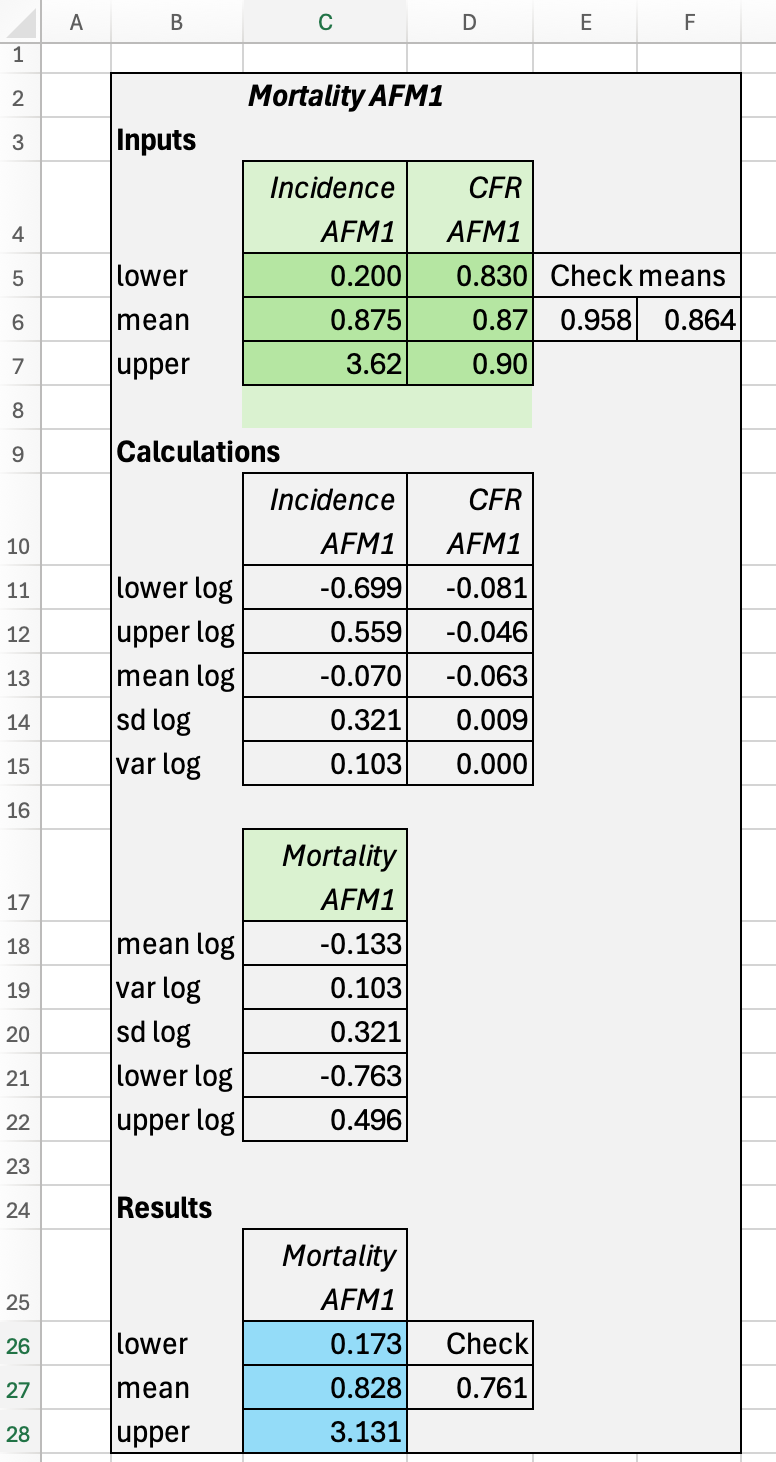
\includegraphics[width=2.59in,height=\textheight,keepaspectratio]{XL_lognormal.png}

}

\caption{\label{fig-XL-lognorm}Multiplication of two lognormal
uncertainty distributions in Excel}

\end{figure}%

The calculations for dividing two distributions are the same as for
multiplying, except that in cell C18, the mean logs of the two input
distributions are subtracted instead of added and in cell D27, the input
means are divided instead of multiplied.

\subsection{Beta distributions}\label{beta-distributions}

Figure~\ref{fig-XL-beta} shows the calculation of quantiles of an
uncertainty distribution for proportions, illustrated by the
case-fatality ratio of liver cancer due to AFM1. It is assumed that this
is the same as for aflatoxin B1 (AFB1) as the cancer caused by these two
hazards is the same. According to FERG data, there were 433 cases of
liver cancer due to AFB1 in Ethiopia in 2010, of which 376 died. These
inputs are entered in cells C5:C6. We use a Bayesian approach to
estimate the parameters and quantiles of a Beta distribution to model
the uncertainty in the case-fatality ratio (\emph{12}). A Beta
distribution is bounded between 0 and 1 and can take many shapes, which
makes it a good choice to model proportions. If there are \(n\) cases
and \(s\) deaths, the Beta distribution defining the uncertainty around
the mean is:

\begin{equation}\phantomsection\label{eq-beta}{
Beta(s+1, n-s+1)
}\end{equation}

The parameters of this distribution are calculated in cells D5:D6. The
mean case-fatality ratio is \((s+1)/(n+2)\), which is calculated in cell
C12. Quantiles of this distribution (i.e., the 2.5, 50 and 97.5
percentiles) can be calculated using the inverse Beta function in
\texttt{Excel}, e.g., \(upper=BETA.INV(0.975,C5,C6)\), and are provided
in cells C10, C11 and C13.

\begin{figure}

\centering{

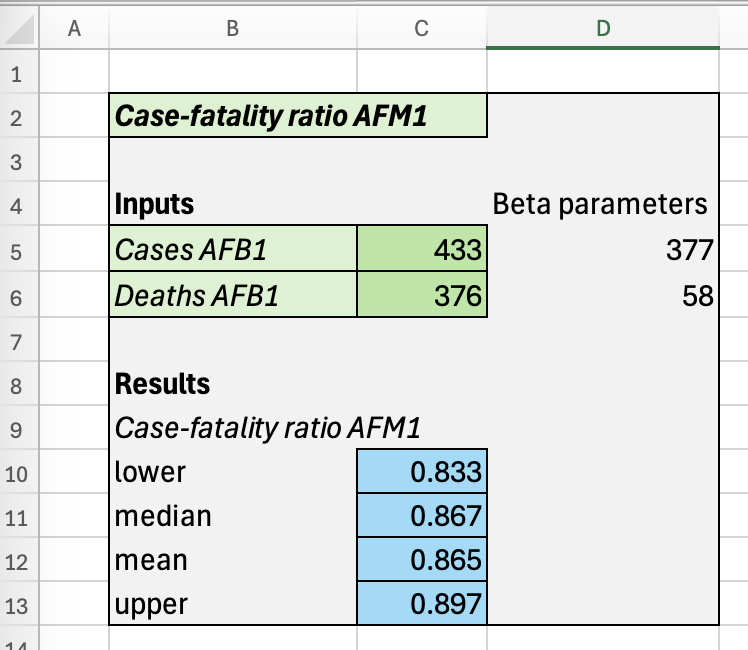
\includegraphics[width=2.49in,height=\textheight,keepaspectratio]{XL_beta.png}

}

\caption{\label{fig-XL-beta}Estimation of quantiles of Beta uncertainty
distribution for proportions}

\end{figure}%

\subsection{Gamma distributions}\label{gamma-distributions}

Figure~\ref{fig-XL-gamma} shows the calculation of quantiles of an
uncertainty distribution for rates, illustrated by the incidence of
anthrax due to infection with \emph{Bacillus anthracis}. According to
(\emph{1}), there were 5,197 human cases of anthrax in Ethiopia in 5
years. These inputs are entered in cells C5:C6. We use a Bayesian
approach to estimate the parameters and quantiles of a Gamma
distribution to model the uncertainty in the incidence rate (\emph{12}).
A Gamma distribution is bounded between 0 and \(\infty\), and is often
used to model rates. If there are \(n\) cases in \(y\) years, the Gamma
distribution defining the uncertainty around the mean is:

\[
Gamma(n, 1/y)
\]

Here, \(n\) is the shape parameter and \(1/y\) the scale parameter. The
parameters of this distribution are calculated in cells D5:D6. The mean
incidence is \(n \times(1/y)\), which is calculated in cell C12.
Quantiles of this distribution (i.e., the 2.5, 50 and 97.5 percentiles)
can be calculated using the inverse Gamma function in \texttt{Excel},
e.g., \(upper=GAMMA.INV(0.975,C5,C6)\), and are provided in cells C10,
C11 and C13.

\begin{figure}

\centering{

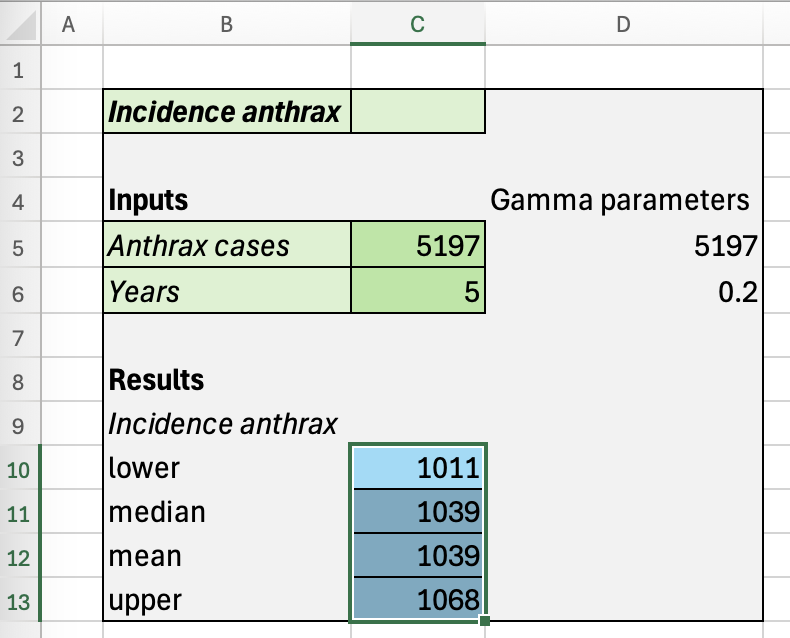
\includegraphics[width=2.63in,height=\textheight,keepaspectratio]{XL_gamma.png}

}

\caption{\label{fig-XL-gamma}Estimation of quantiles of Gamma
uncertainty distribution for rates}

\end{figure}%

\section{Disease burden dashboard}\label{disease-burden-dashboard}

The disease burden dashboard was created to provide users with a
friendly, yet comprehensive way of visualizing, and comparing data on
disease burden of FERG hazards. Features include multiple ways of
graphing hazard data, multiple scaling options and fine-grained
capability to compare a subset of hazards side by side. It has since
expanded to generate and graph data for additional hazards through a
user accessible simulation. This functionality has been used to add the
burden of non-FER hazards selected by Ethiopina stakehoilders to the
dashboard. In addition, users are able to run the simulation on data
collected for custom hazards of chocie and feed the results back into
the dashboard to be visualized alongside the other hazards.

The plots, graphical interface and simulations were created in R
statistical software using the Shiny and ggplot2 packages. The dashboard
can be accessed at
\url{https://osu-cfi.shinyapps.io/ethdashboard/}\href{https://osu-cfi.shinyapps.io/ethdashboard/.}{.}

The following sections describe the data, terminology and features of
the dashboard.

\subsection{Data}\label{data}

This section discusses how the data in the dashboard was collected and
used, and relevant definitions.

\subsubsection{Data Collection and
Usage}\label{data-collection-and-usage}

The dashboard graphically plots two different data sets. The first data
set, referred to as FERG Hazards in the following sections, contains
Ethiopian estimates of foodborne disease burden attributed to various
hazards obtained from FERG report. The second data set, referred to as
non-FERG hazards, contains data on hazards that did not have FERG
estimates available but were prioritized by the Ethiopian stakeholders.
Monte Carlo samples for the dashboard were generated using the `Minimum
Quantile Information Distribution' in the \texttt{mc2d} package. This
distribution uses linear interpolation between three defined quantiles
to construct a cumulative distribution function (cdf) (\emph{3}). The
minimum and maximum of the cdf are defined by an overshoot \(k\), i.e.,
the cdf is expanded on both sides by \(k \%\) of the range between the
lower and upper quantiles.

\begin{Shaded}
\begin{Highlighting}[]
\DocumentationTok{\#\# The rmqi function needs three inputs: }
  \CommentTok{\# mqi, a vector of three cumulative proability values}
  \CommentTok{\# n, the number of samples to be generated}
  \CommentTok{\# mqi.quantile, a vector of the quantiles}

\FunctionTok{set.seed}\NormalTok{(}\DecValTok{48814}\NormalTok{) }\CommentTok{\# generated at random.org using Min: 1,  Max: 100000; 2022 {-} 05 {-} 18 20:14:30 UTC}

\CommentTok{\# Generate mqi vector list from NonFERG\_data object}
\NormalTok{mqis }\OtherTok{\textless{}{-}} \FunctionTok{map}\NormalTok{(}\FunctionTok{transpose}\NormalTok{(NonFERG\_data[, }\DecValTok{4}\SpecialCharTok{:}\DecValTok{6}\NormalTok{]), unlist)}
\CommentTok{\# Then we generate n and mqi.quantile lists}
\NormalTok{n }\OtherTok{\textless{}{-}} \FunctionTok{rep}\NormalTok{(}\DecValTok{10000}\NormalTok{, }\FunctionTok{nrow}\NormalTok{(NonFERG\_data))}
\NormalTok{mqi.quantile }\OtherTok{\textless{}{-}} \FunctionTok{rep}\NormalTok{(}\FunctionTok{list}\NormalTok{(}\FunctionTok{c}\NormalTok{(}\FloatTok{0.025}\NormalTok{, }\FloatTok{0.5}\NormalTok{, }\FloatTok{0.975}\NormalTok{)), }\FunctionTok{nrow}\NormalTok{(NonFERG\_data))}
\CommentTok{\# Use pmap to generate random samples}
\NormalTok{NonFERG\_samples }\OtherTok{\textless{}{-}} \FunctionTok{pmap}\NormalTok{(}\FunctionTok{list}\NormalTok{(}\AttributeTok{mqi=}\NormalTok{mqis, }\AttributeTok{n=}\NormalTok{n, }\AttributeTok{mqi.quantile=}\NormalTok{mqi.quantile), rmqi)}
\CommentTok{\# Create data frame with samples and identifiers}
\end{Highlighting}
\end{Shaded}

\subsubsection{Risk Metric Definitions}\label{sec-metrics}

Each hazard in both data sets listed above have multiple risk metrics
that describe it. The dashboard allows users to select which metric to
visualize. The definitions of each metric are listed below:

\begin{itemize}
\item
  Incidence -- Number of new cases of disease during a specified time
  interval.
\item
  Incidence\_Rate\_100K -- Incidence rate per 100,000 people per year.
\item
  Mortality - Number of new deaths that occur during during a specified
  time interval.
\item
  Mortality\_Rate\_100K --The number of deaths per 100,000 people per
  year.
\item
  Disability-Adjusted Life Year (DALY) - A health gap measure that
  combines the years of life lost due to premature death (YLL) and the
  years lived with disability (YLD) from a disease or condition, for
  varying degrees of severity, making time itself the common metric for
  death and disability. One DALY equates to 1 year of healthy life lost.
\item
  DALY\_Rate\_100K - The number of DALYs per 100,000 peole per year.
\item
  Case\_Fatality\_ratio - Proportion of people who die from a specified
  disease among all individuals diagnosed with the disease over a
  certain period of time.
\item
  DALY\_per\_case - Number of DALYs divided by incidence.
\item
  Years of Life Lost (YLL) -- The number of deaths due to a specific
  disease or condition multiplied by the standard life expectancy at the
  age at which death occurs.
\item
  Years Lived with Disability (YLD) -- Number of years lived with a
  disability due to a specific disease or condition multiplied by a
  diasability weight.
\end{itemize}

\subsection{Features}\label{features}

\subsubsection{All Hazards Tab}\label{all-hazards-tab}

The All Hazards Tab by default displays all of the FERG and Non-FERG
hazards in a single set of box plots. As shown below in
Figure~\ref{fig-all-hazards}, the red box plots denote FERG hazards and
the blue box plots denote the Non-FERG hazards.

\begin{figure}

\centering{

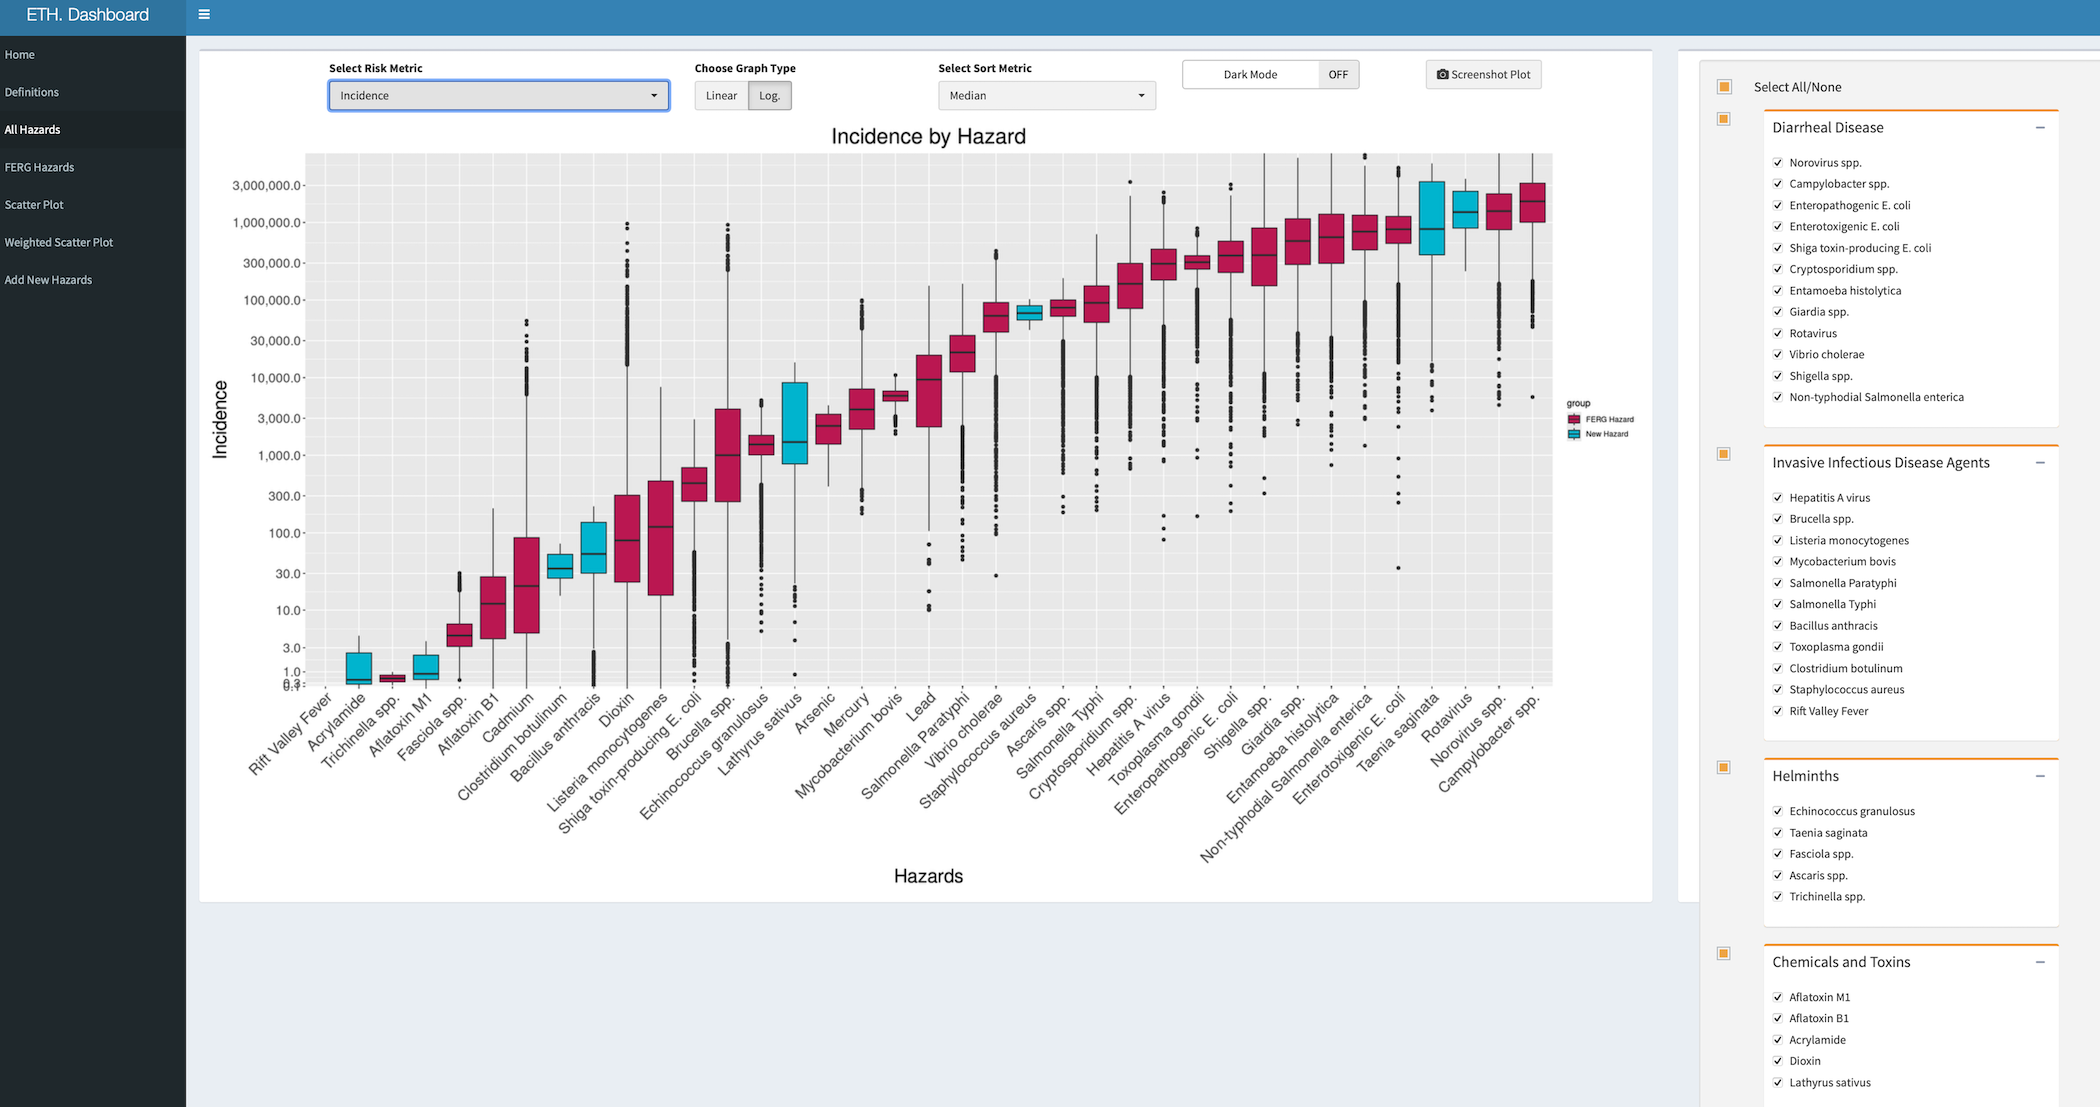
\includegraphics[width=7in,height=\textheight,keepaspectratio]{allhazards.png}

}

\caption{\label{fig-all-hazards}All Hazards tab}

\end{figure}%

The top left drop-down box labeled ``Select Risk Metric'' allows users
to choose from the following risk metrics to display on the y-axis
defined in Section~\ref{sec-metrics}:

\begin{itemize}
\tightlist
\item
  Incidence
\item
  Mortality
\item
  DALYs
\item
  Incidence\_Rate\_100K
\item
  Mortality\_Rate\_100K
\item
  DALY\_Rate\_100K
\item
  Case\_Fatality\_ratio
\item
  DALY\_per\_case
\end{itemize}

The ``Choose Graph Type'' select box switches the y-axis between a
logarithmic and linear scale. The default scale is the log scale.

The ``Select Sort Metric'' allows users to sort the x-axis based on the
alphabetical order of hazard names or the median risk metric value. The
default sort metric is the median i.e.~the hazards on the x-axis are
ordered such that the hazard's median value is increasing.

Two additional boxes allow the user to select Dark Mode, and to create a
screenshot of the plot for future reference.

Finally, the checkboxes on the right hand side allow users to select
which hazards to plot. Two levels of granularity are given: users are
able to select/deselect individual hazards one at a time or by entire
hazard groups. Hazard groups include Diarrheal Disease Agents, Invasive
Infectious Disease Agents, Helminths, Chemicals and Toxins and Metals.

Figure~\ref{fig-allhazards_select} below is an example where we only
want to compare Helminths and Metals and choose specific hazards within
these two groups.

\begin{figure}

\centering{

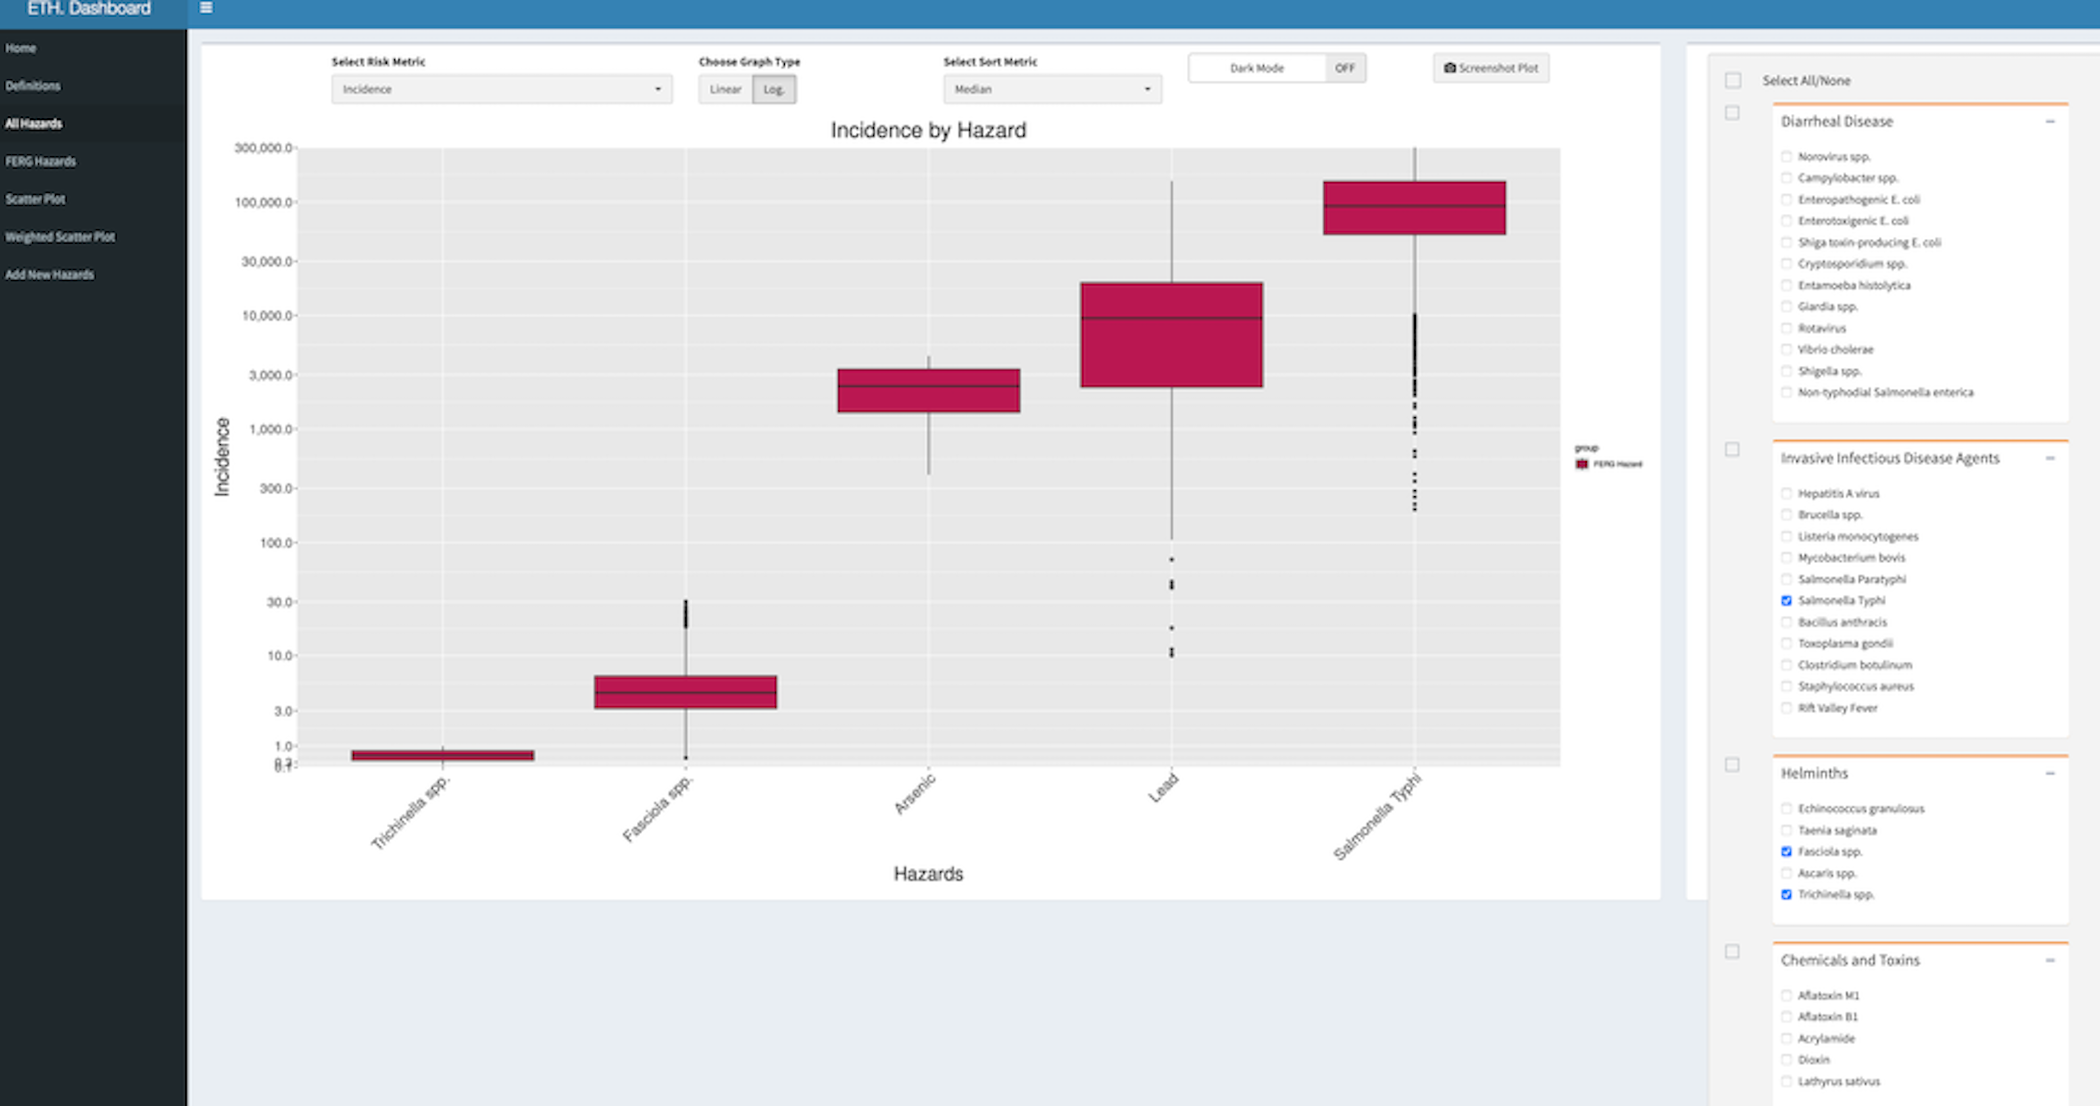
\includegraphics[width=7in,height=\textheight,keepaspectratio]{allhazards_select.png}

}

\caption{\label{fig-allhazards_select}All Hazards tab selection}

\end{figure}%

\subsubsection{FERG Hazards}\label{ferg-hazards}

THe FERG Hazards tab displays the data for the FERG hazards only. The
layout and functionality is the same as the All Hazards tab. FERG
disease burden estimates are available for the total population as well
as for two age groups (children under 5 years of age and people over 5
years of age). An additional drop-down box Select Dataset is provided to
allow users to choose between the two datasets.

\subsubsection{Scatter Plot}\label{scatter-plot}

The Scatterplot tab allows users to create two-dimensional plots of the
data by choosing different metrics for the x-axis and y-axis, see
Figure~\ref{fig-scatter}. This allows users to explore, for example, the
two dimensions of risk (e.g.~incidence as a metric of likelihood and
DALYs per case as a metric of severity) for each hazard.The scatterplot
is labeled by hazard names, color coded by Hazard Group. The user can
select the x-axis and y-axis metrics from the dropdown menus. The user
can also select the metrics on both axes as well as the dataset using
the Graph Options drop-down box.

\begin{figure}

\centering{

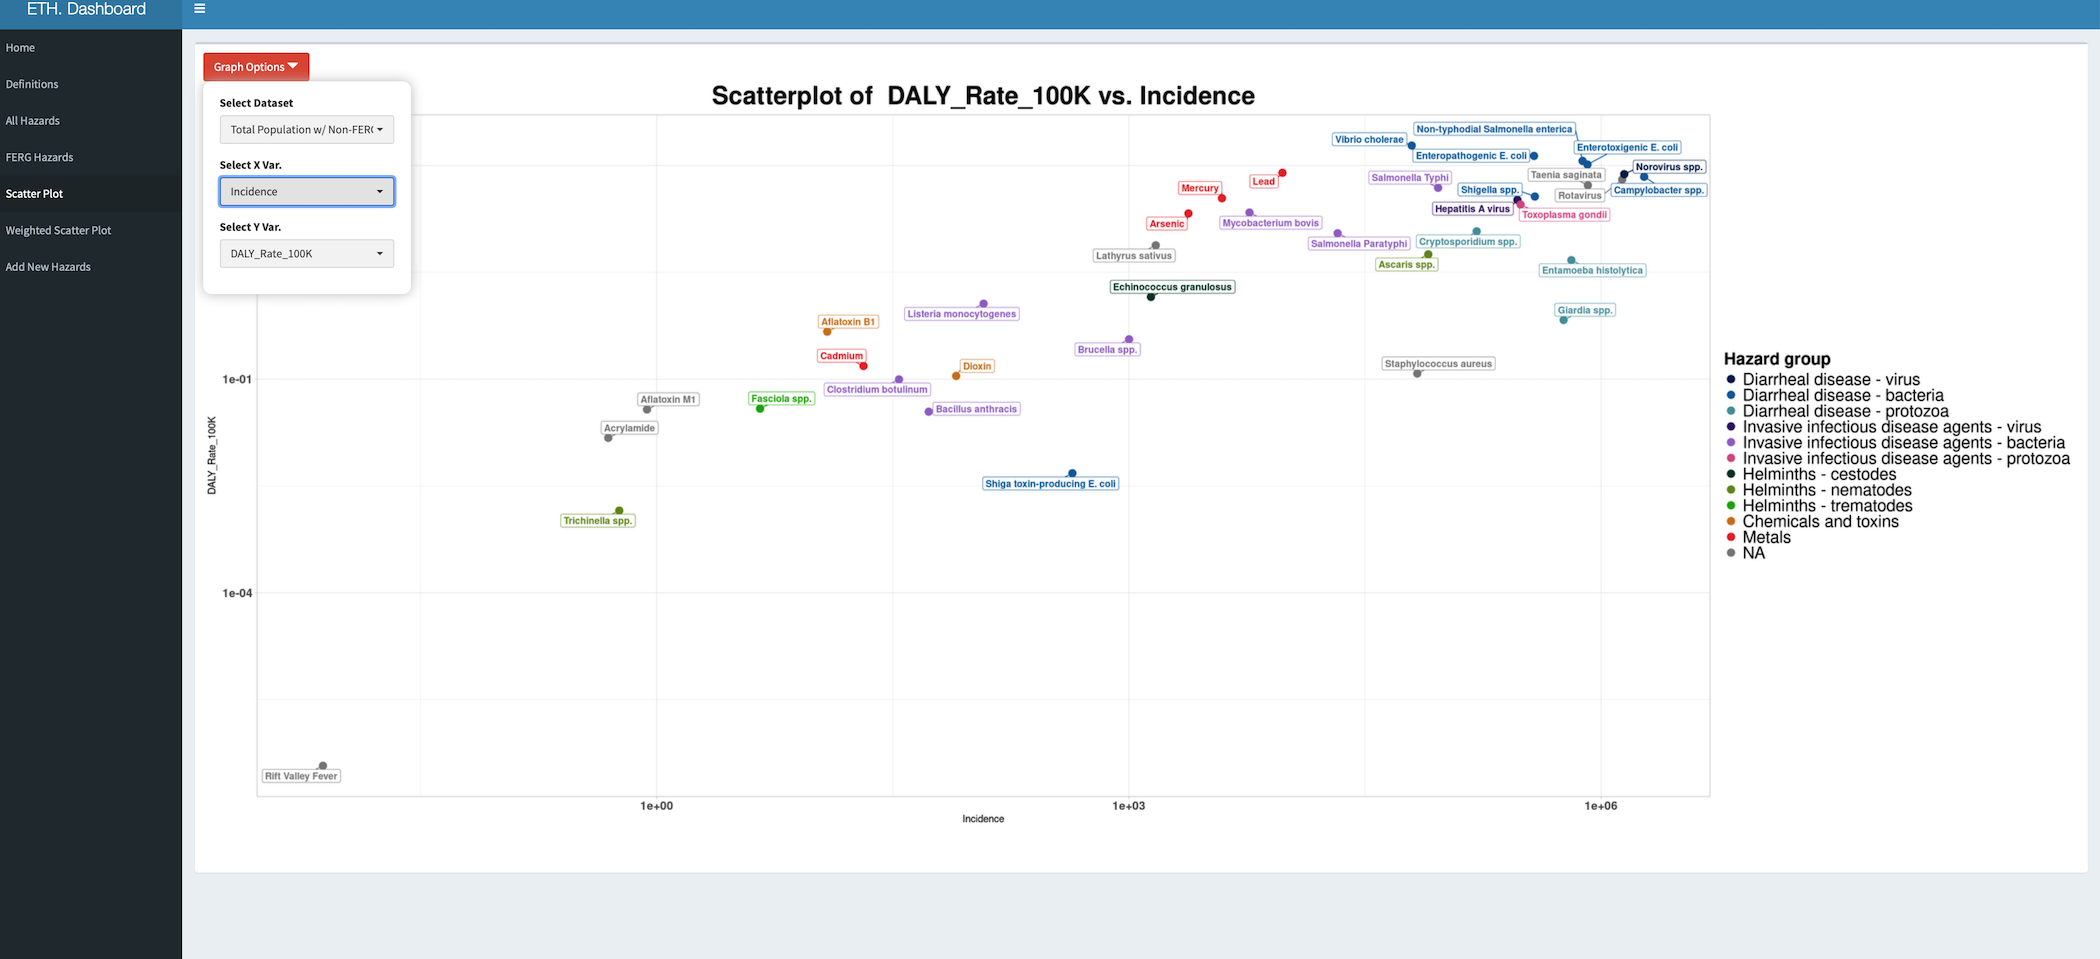
\includegraphics[width=7in,height=\textheight,keepaspectratio]{scatter.png}

}

\caption{\label{fig-scatter}Scatter Plot tab}

\end{figure}%

\subsubsection{Weighted Scatter Plot}\label{weighted-scatter-plot}

The Weighted Scatterplot (Figure~\ref{fig-w-scatter}) allows the user to
add a third dimension to the plot, with the chosen metric for the third
dimension being used to calculate the size of the dots. The
functionality is otherwise the same as for the Scatter Plot.

\begin{figure}

\centering{

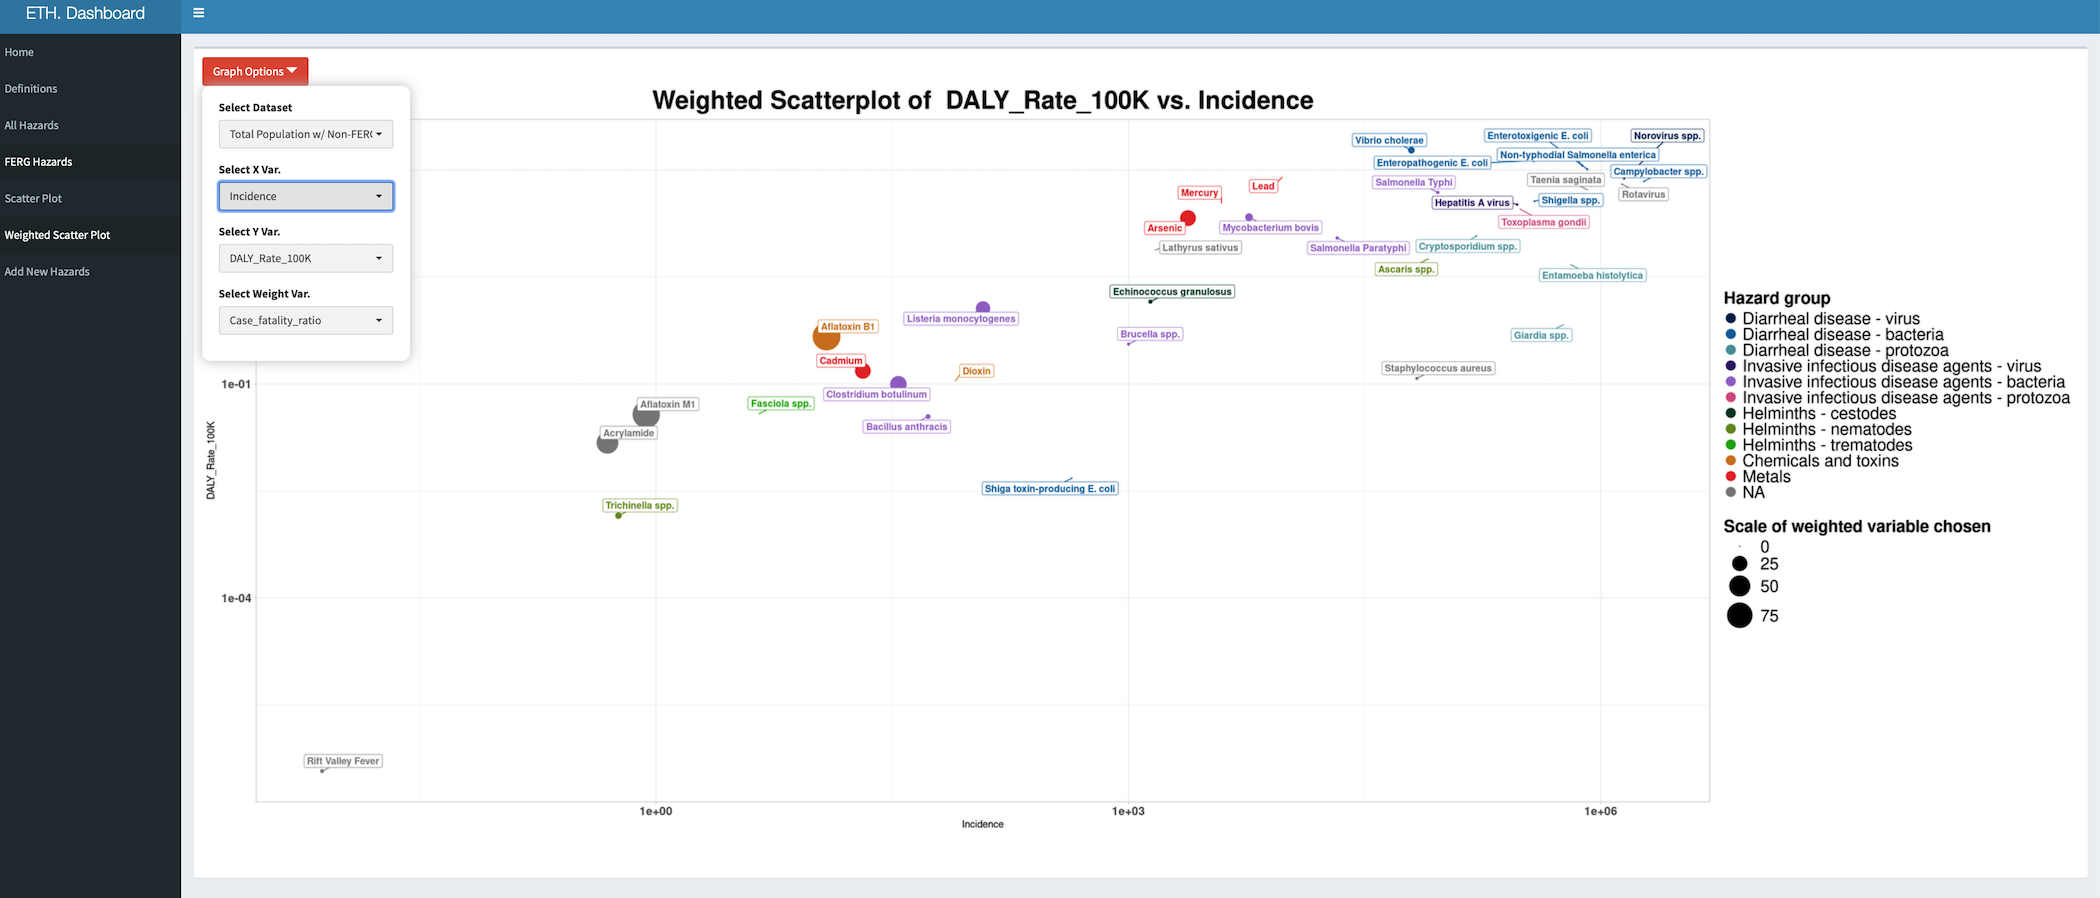
\includegraphics[width=7in,height=\textheight,keepaspectratio]{w-scatter.png}

}

\caption{\label{fig-w-scatter}Weighted Scatter Plot tab}

\end{figure}%

\subsubsection{Add New Hazards}\label{add-new-hazards}

The Add New Hazards tab allows users to generate data for custom
hazards. Detaile dinstructions are provided on the web page
(Figure~\ref{fig-simulation}).

\begin{figure}

\centering{

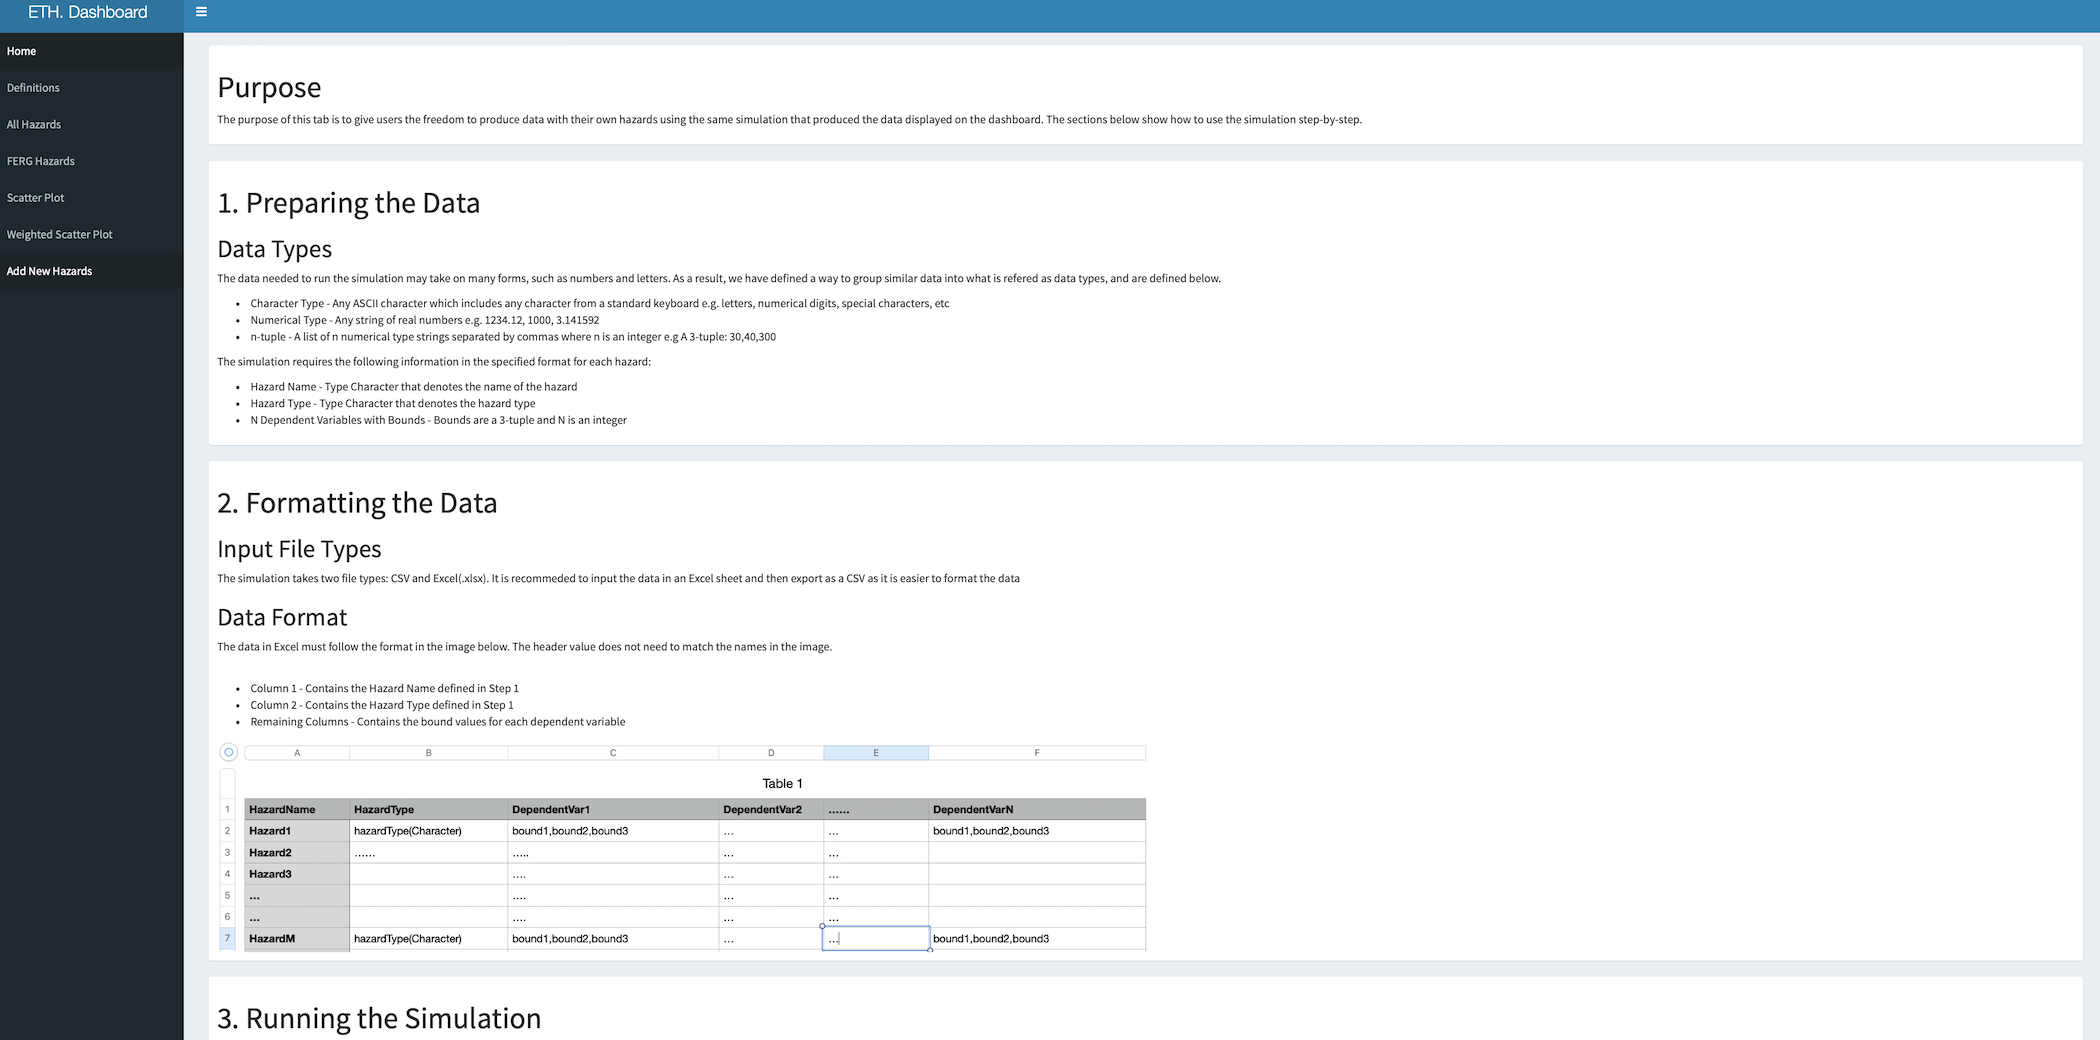
\includegraphics[width=7in,height=\textheight,keepaspectratio]{simulation.png}

}

\caption{\label{fig-simulation}Add New Hazards tab}

\end{figure}%

The simulation consists of three steps:

\begin{enumerate}
\def\labelenumi{\arabic{enumi}.}
\item
  Gathering and Preparing the Data

  The simulation requires the lower,middle and upper distribution value
  of each hazard. These should be formatted as in
  Figure~\ref{fig-simulation-input}.
\item
  Formatting the Data

  Once all the distribution values have been calculated, the data must
  be formatted in an Excel or CSV file. The exact format can be found in
  the second select tab labelled ``2. Formatting the Data''.
\item
  Upload and Running the Simulation

  The final step is to upload the formatted Excel or CSV file and
  pressing the ``Run and Download'' button.
\end{enumerate}

The resulting data from the simulation can then be plotted in the
dashboard.

\begin{figure}

\centering{

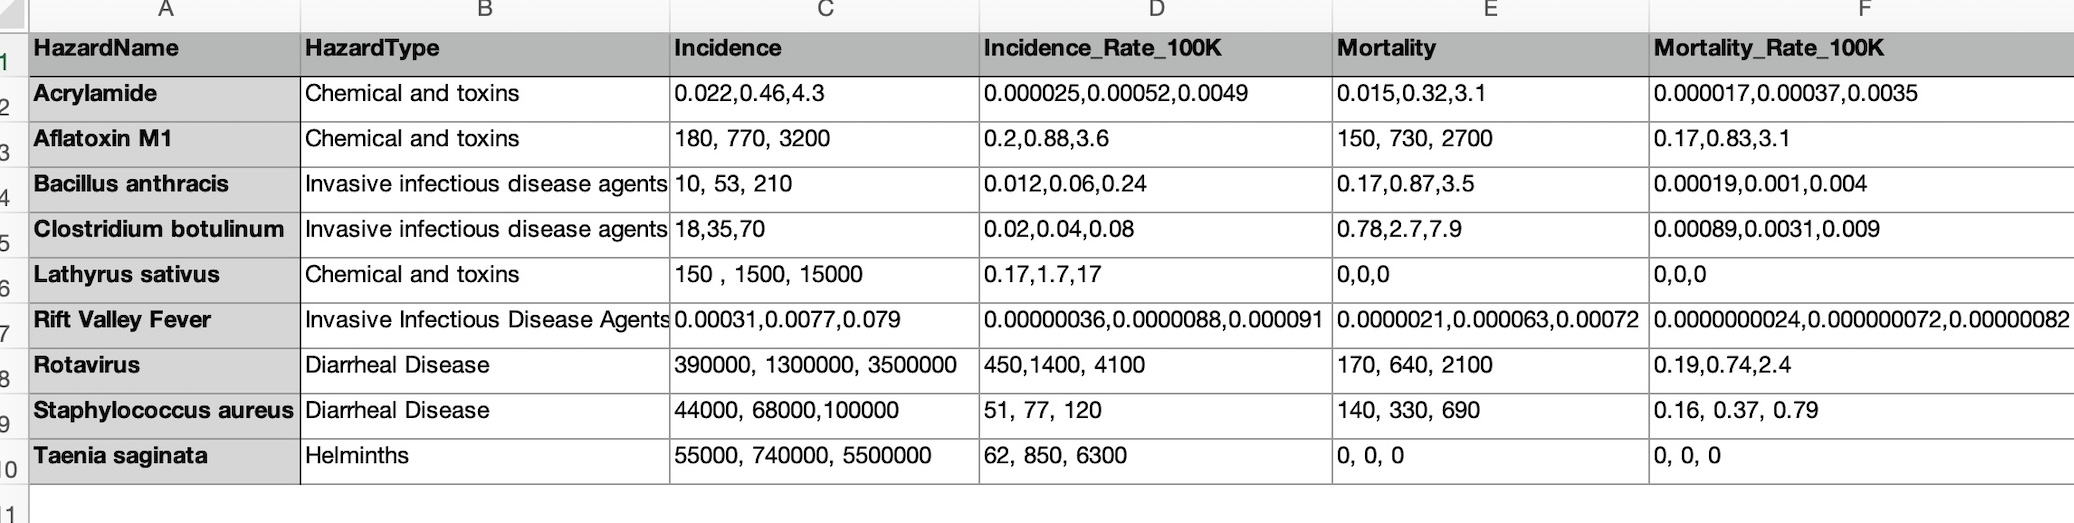
\includegraphics[width=7.73in,height=\textheight,keepaspectratio]{simulation-input.jpeg}

}

\caption{\label{fig-simulation-input}Format to import data on custom
hazards in dashboard}

\end{figure}%

\section{Risk ranking}\label{risk-ranking}

\subsection{Methods}\label{methods}

Data from the first two rounds of the risk ranking workshop were
collected in spreadsheets and merged into a single dataset. All data
extraction, manipulation, plots and statistical testing were generated
in \textbf{R} statistical software (\emph{6}), using the \texttt{dplyr}
package (\emph{14}) for data processing. The final dataset is available
in file \texttt{rr\_dat.rds}.

Descriptive statistics of the risk ranking results included
cross-tabulations and stacked bar-charts using the \texttt{ggplot2}
package (\emph{13}) while mosaic plots were prepared using the
\texttt{ggmosaic} package (\emph{5}). Univariate and multivariate
ordinal logistic regression models were created using the \texttt{polr}
function in the \texttt{MASS} package (\emph{9}). The \texttt{GGally}
(\emph{8}) package was used to visually check for multicollinearity.
Model selection was based on the Akaike Information Criterion. The
proportional odds assumption was checked using the Brant test. The final
model was used to identify variables that were most predictive of the
rank in round 2. Information on the software versions used is provided
in the Session Information at the end of this document.

\subsection{Results}\label{results-1}

\subsubsection{Descriptive analysis}\label{descriptive-analysis}

\begin{Shaded}
\begin{Highlighting}[]
\DocumentationTok{\#\#\# READ PROCESSED DATA}
\NormalTok{rr\_dat }\OtherTok{\textless{}{-}} \FunctionTok{readRDS}\NormalTok{(}\StringTok{"rr\_dat.rds"}\NormalTok{)}
\NormalTok{rr\_dat}\SpecialCharTok{$}\NormalTok{hazard }\OtherTok{\textless{}{-}} \FunctionTok{fct\_rev}\NormalTok{(rr\_dat}\SpecialCharTok{$}\NormalTok{hazard) }\CommentTok{\# reverse order of levels for proper arrangement in plots}
\NormalTok{haz\_labels }\OtherTok{\textless{}{-}} \FunctionTok{rev}\NormalTok{(}\FunctionTok{c}\NormalTok{(}\StringTok{"Acrylamide"}\NormalTok{, }\StringTok{"Aflatoxin B1"}\NormalTok{, }\StringTok{"Aflatoxin M1"}\NormalTok{, }\StringTok{"Arsenic"}\NormalTok{, }\StringTok{"Ascaris spp."}\NormalTok{,}
                     \StringTok{"Bacillus anthracis"}\NormalTok{, }\StringTok{"Brucella spp."}\NormalTok{, }\StringTok{"Clostridium botulinum toxins"}\NormalTok{, }\StringTok{"Cadmium"}\NormalTok{,}
                     \StringTok{"Campylobacter spp."}\NormalTok{, }\StringTok{"Cryptosporidium spp."}\NormalTok{, }\StringTok{"Dioxins"}\NormalTok{, }\StringTok{"Echinococcus granulosus"}\NormalTok{,}
                     \StringTok{"Entamoeba spp."}\NormalTok{, }\StringTok{"enteropathogenic Escherichia coli"}\NormalTok{, }\StringTok{"enterotoxigenic E. coli"}\NormalTok{,}
                     \StringTok{"Fasciola spp."}\NormalTok{, }\StringTok{"Giardia spp."}\NormalTok{, }\StringTok{"Hepatitis A virus"}\NormalTok{, }\StringTok{" Lathyrus sativus"}\NormalTok{, }\StringTok{"Lead"}\NormalTok{,}
                     \StringTok{"Listeria monocytogenes"}\NormalTok{, }\StringTok{"Mycobacterium bovis"}\NormalTok{, }\StringTok{"Methylmercury"}\NormalTok{, }\StringTok{"Norovirus"}\NormalTok{,}
                     \StringTok{"Rift Valley Fever virus"}\NormalTok{, }\StringTok{"Rotavirus"}\NormalTok{, }\StringTok{"Staphylococcus aureus enterotoxins"}\NormalTok{,}
                     \StringTok{"Salmonella Paratyphi"}\NormalTok{, }\StringTok{"Salmonella Typhi"}\NormalTok{, }\StringTok{"nontyphoidal Salmonella enterica"}\NormalTok{,}
                     \StringTok{"Shigella spp."}\NormalTok{,}\StringTok{"Shiga{-}toxin producing E. coli"}\NormalTok{, }\StringTok{"Taenia saginata"}\NormalTok{, }\StringTok{"Toxoplasma gondii"}\NormalTok{,}
                     \StringTok{"Trichinella spp."}\NormalTok{, }\StringTok{"Vibrio cholerae"}\NormalTok{)) }\CommentTok{\# reverse order of legends}

\DocumentationTok{\#\#\# Stacked bar charts}

\NormalTok{rank1 }\OtherTok{\textless{}{-}} \FunctionTok{ggplot}\NormalTok{(rr\_dat, }\FunctionTok{aes}\NormalTok{(}\AttributeTok{x =}\NormalTok{ hazard, }\AttributeTok{fill =}\NormalTok{ rank1)) }\SpecialCharTok{+}
    \FunctionTok{geom\_bar}\NormalTok{(}\AttributeTok{position =} \StringTok{"stack"}\NormalTok{, }\AttributeTok{stat =} \StringTok{"count"}\NormalTok{) }\SpecialCharTok{+}
    \FunctionTok{labs}\NormalTok{(}\AttributeTok{x =} \StringTok{"Hazard"}\NormalTok{, }\AttributeTok{y =} \StringTok{"Count"}\NormalTok{, }\AttributeTok{fill =} \StringTok{"Rank"}\NormalTok{) }\SpecialCharTok{+}
    \FunctionTok{scale\_fill\_brewer}\NormalTok{(}\AttributeTok{palette =} \StringTok{"Set2"}\NormalTok{) }\SpecialCharTok{+}
    \FunctionTok{coord\_flip}\NormalTok{() }\SpecialCharTok{+}
    \FunctionTok{scale\_x\_discrete}\NormalTok{(}\AttributeTok{labels =}\NormalTok{ haz\_labels)}

\FunctionTok{ggsave}\NormalTok{(}\AttributeTok{filename =} \StringTok{"rank1"}\NormalTok{, }\AttributeTok{plot =}\NormalTok{ rank1, }\AttributeTok{device =} \StringTok{"tiff"}\NormalTok{, }\AttributeTok{width =} \DecValTok{3}\NormalTok{, }\AttributeTok{height =} \DecValTok{2}\NormalTok{, }\AttributeTok{unit =} \StringTok{"in"}\NormalTok{, }\AttributeTok{dpi =} \DecValTok{300}\NormalTok{)}

\NormalTok{rank2 }\OtherTok{\textless{}{-}} \FunctionTok{ggplot}\NormalTok{(rr\_dat, }\FunctionTok{aes}\NormalTok{(}\AttributeTok{x =}\NormalTok{ hazard, }\AttributeTok{fill =}\NormalTok{ rank2)) }\SpecialCharTok{+}
    \FunctionTok{geom\_bar}\NormalTok{(}\AttributeTok{position =} \StringTok{"stack"}\NormalTok{, }\AttributeTok{stat =} \StringTok{"count"}\NormalTok{) }\SpecialCharTok{+}
    \FunctionTok{labs}\NormalTok{(}\AttributeTok{x =} \StringTok{"Hazard"}\NormalTok{, }\AttributeTok{y =} \StringTok{"Count"}\NormalTok{, }\AttributeTok{fill =} \StringTok{"Rank"}\NormalTok{) }\SpecialCharTok{+}
     \FunctionTok{scale\_fill\_brewer}\NormalTok{(}\AttributeTok{palette =} \StringTok{"Set2"}\NormalTok{) }\SpecialCharTok{+}
    \FunctionTok{coord\_flip}\NormalTok{() }\SpecialCharTok{+}
    \FunctionTok{scale\_x\_discrete}\NormalTok{(}\AttributeTok{labels =}\NormalTok{ haz\_labels)}

\FunctionTok{ggsave}\NormalTok{(}\AttributeTok{filename =} \StringTok{"rank2"}\NormalTok{, }\AttributeTok{plot =}\NormalTok{ rank1, }\AttributeTok{device =} \StringTok{"tiff"}\NormalTok{, }\AttributeTok{width =} \DecValTok{3}\NormalTok{, }\AttributeTok{height =} \DecValTok{2}\NormalTok{, }\AttributeTok{unit =} \StringTok{"in"}\NormalTok{, }\AttributeTok{dpi =} \DecValTok{300}\NormalTok{)}

\DocumentationTok{\#\#\# Mosaic plots}

\NormalTok{mosaic\_r12 }\OtherTok{\textless{}{-}} \FunctionTok{ggplot}\NormalTok{(}\AttributeTok{data =}\NormalTok{ rr\_dat) }\SpecialCharTok{+}
    \FunctionTok{geom\_mosaic}\NormalTok{(}\FunctionTok{aes}\NormalTok{(}\AttributeTok{x =} \FunctionTok{product}\NormalTok{(rank2, rank1), }\AttributeTok{fill =}\NormalTok{ rank2)) }\SpecialCharTok{+}
    \FunctionTok{scale\_fill\_brewer}\NormalTok{(}\AttributeTok{palette =} \StringTok{"Set2"}\NormalTok{) }\SpecialCharTok{+}
    \FunctionTok{labs}\NormalTok{(}\AttributeTok{y=}\StringTok{"Round 2"}\NormalTok{, }\AttributeTok{x=}\StringTok{"Round 1"}\NormalTok{, }\AttributeTok{fill =} \StringTok{"Rank"}\NormalTok{)}

\FunctionTok{ggsave}\NormalTok{(}\AttributeTok{filename =} \StringTok{"mosaic\_r12"}\NormalTok{, }\AttributeTok{plot =}\NormalTok{ rank1, }\AttributeTok{device =} \StringTok{"tiff"}\NormalTok{, }\AttributeTok{width =} \DecValTok{3}\NormalTok{, }\AttributeTok{height =} \DecValTok{2}\NormalTok{, }\AttributeTok{unit =} \StringTok{"in"}\NormalTok{, }\AttributeTok{dpi =} \DecValTok{300}\NormalTok{)}

\NormalTok{mosaic\_r12\_sub }\OtherTok{\textless{}{-}} \FunctionTok{ggplot}\NormalTok{(}\AttributeTok{data =}\NormalTok{ rr\_dat) }\SpecialCharTok{+}
    \FunctionTok{geom\_mosaic}\NormalTok{(}\FunctionTok{aes}\NormalTok{(}\AttributeTok{x =} \FunctionTok{product}\NormalTok{(rank2, rank1), }\AttributeTok{fill =}\NormalTok{ rank2)) }\SpecialCharTok{+}
    \FunctionTok{scale\_fill\_brewer}\NormalTok{(}\AttributeTok{palette =} \StringTok{"Set2"}\NormalTok{) }\SpecialCharTok{+}
    \FunctionTok{labs}\NormalTok{(}\AttributeTok{y=}\StringTok{"Round 2"}\NormalTok{, }\AttributeTok{x=}\StringTok{"Round 1"}\NormalTok{, }\AttributeTok{fill =} \StringTok{"Rank"}\NormalTok{) }\SpecialCharTok{+}
    \FunctionTok{facet\_wrap}\NormalTok{(}\SpecialCharTok{\textasciitilde{}}\NormalTok{metric1, }
               \AttributeTok{labeller =} \FunctionTok{labeller}\NormalTok{(}\AttributeTok{metric1 =} \FunctionTok{c}\NormalTok{(}\StringTok{"daly"} \OtherTok{=} \StringTok{"DALYs"}\NormalTok{, }\StringTok{"incidence"} \OtherTok{=} \StringTok{"Incidence"}\NormalTok{, }\StringTok{"cfr"} \OtherTok{=} \StringTok{"Case{-}Fatality Ratio"}\NormalTok{, }\StringTok{"mortality"} \OtherTok{=} \StringTok{"Mortality"}\NormalTok{)))}

\FunctionTok{ggsave}\NormalTok{(}\AttributeTok{filename =} \StringTok{"mosaic\_r12\_sub"}\NormalTok{, }\AttributeTok{plot =}\NormalTok{ rank1, }\AttributeTok{device =} \StringTok{"tiff"}\NormalTok{, }\AttributeTok{width =} \DecValTok{3}\NormalTok{, }\AttributeTok{height =} \DecValTok{2}\NormalTok{, }\AttributeTok{unit =} \StringTok{"in"}\NormalTok{, }\AttributeTok{dpi =} \DecValTok{300}\NormalTok{)}
\end{Highlighting}
\end{Shaded}

The ranking results for each hazard in round 1 are shown in
Figure~\ref{fig-round1}. There were five hazards that were assigned the
same rank by all groups (High: \emph{Mycobacterium bovis}, Medium:
Shiga-toxin producing \emph{Escherichia coli} and \emph{Trichinella}
spp., Low: \emph{Echinococcus granulosus} and Rift Valley Fever virus)
and these ranks were considered final.

\begin{figure}

\centering{

\pandocbounded{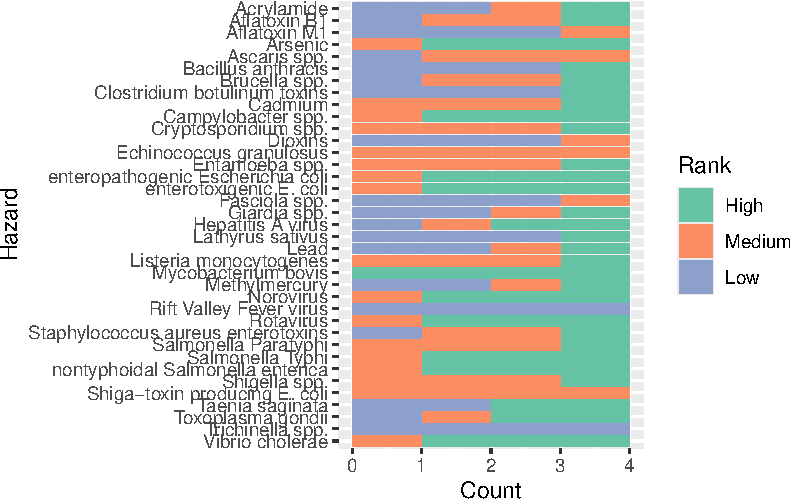
\includegraphics[keepaspectratio]{RR_TechApp_files/figure-pdf/fig-round1-1.pdf}}

}

\caption{\label{fig-round1}Risk ranking results in round 1}

\end{figure}%

In round 2, groups ranked 32 hazards and five ranks were carried over
from round 1. Overall changes in ranking are visualized in
Figure~\ref{fig-mosaic-round2}. There was a high number of hazards that
were ranked Low in both rounds but changes from Low to Medium did occur.
Changes from Low to High did not occur. Most hazards that were ranked
Medium in round 1 were also ranked Medium in round 2, but changes
occurred to both Low and High ranks. Most changes in ranking occurred
for hazards that were ranked High in round 1, changing to Medium or even
Low ranks.

\begin{figure}

\centering{

\pandocbounded{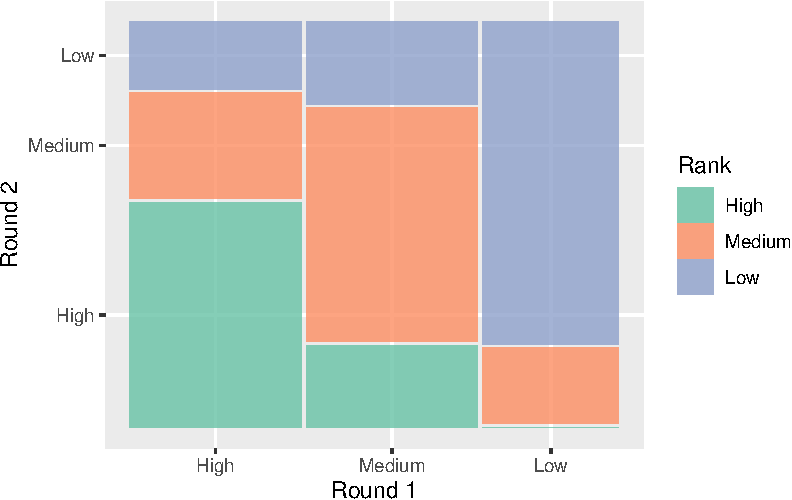
\includegraphics[keepaspectratio]{RR_TechApp_files/figure-pdf/fig-mosaic-round2-1.pdf}}

}

\caption{\label{fig-mosaic-round2}Changes in ranking from round 1 to
round 2}

\end{figure}%

A more detailed analysis of changes in ranking from round 1 to round 2
per metric used in round 1 is presented in
Figure~\ref{fig-mosaic-round2sub}. The group that used incidence as the
metric in round 1 changed 20 out of 33 rankings. Hazards with High or
Medium rank were reassigned to the same categories but with relatively
many crossovers and some hazards were moved from Low to Medium rank. The
group using mortality as metric in round 1 changed 27 out of 33
rankings, mainly Medium and Low ranks in round 1. The group using
case-fatality ratio as metric in round 1 changed 22 out of 33 ranking,
mainly crossovers between High and Medium. The group using DALYs as
metric in round 1 changed 26 out of 33 rankings, mainly downranking
hazards ranked as High or Medium in round 1.

\begin{figure}

\centering{

\pandocbounded{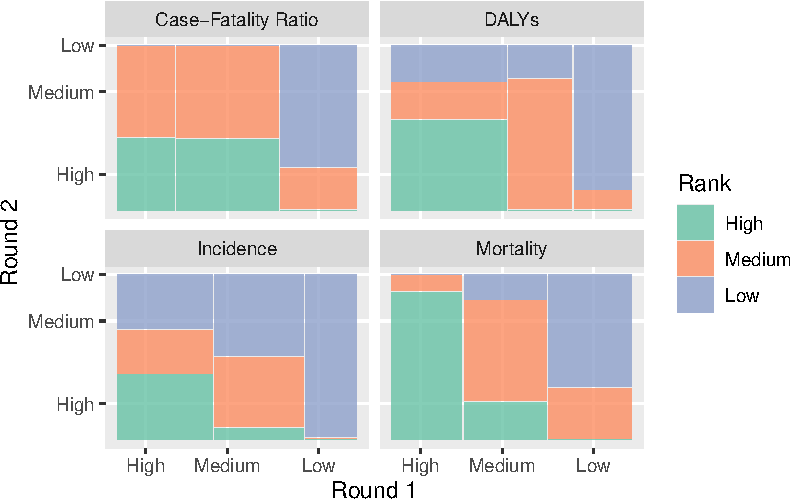
\includegraphics[keepaspectratio]{RR_TechApp_files/figure-pdf/fig-mosaic-round2sub-1.pdf}}

}

\caption{\label{fig-mosaic-round2sub}Changes in ranking from round 1 to
round 2 by metric assigned to groups in round 1}

\end{figure}%

The ranking results for each hazard following round 2 are shown in
Figure~\ref{fig-round2}. There were fifteen hazards that were assigned
the same rank by all groups (High: enterotoxigenic \emph{Escherichia
coli}, \emph{Mycobacterium bovis},rotavirus, \emph{Salmonella enterica}
subsp. \emph{enterica} (non-typhoidal) and \emph{Vibrio cholerae};
Medium: \emph{Cryptosporidium} spp., \emph{Echinococcus granulosus},
\emph{Salmonella enterica} subsp. \emph{enterica} serovar Paratyphi and
Shiga-toxin producing \emph{Escherichia coli}; Low: dioxins,
\emph{Fasciola} spp., \emph{Lathyrus sativus}, Rift Valley Fever virus,
\emph{Taenia saginata} and \emph{Trichinella} spp.) and these ranks were
considered final.

\begin{figure}

\centering{

\pandocbounded{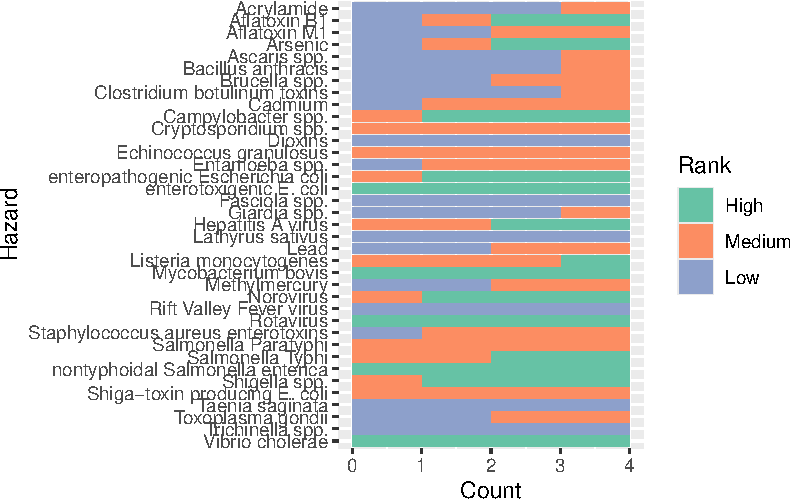
\includegraphics[keepaspectratio]{RR_TechApp_files/figure-pdf/fig-round2-1.pdf}}

}

\caption{\label{fig-round2}Risk ranking results in round 2}

\end{figure}%

Ranking of hazards for which no agreement was reached after round 2 were
finalized by group discussions as described in the main text.

\subsubsection{Ordinal logistic
regression}\label{ordinal-logistic-regression}

In the univariate analysis, all predictor variables were highly
significant (Table~\ref{tbl-uni}). The multivariate model was developed
using backward selection, starting with the model including all
significant variables in the univariate analysis. There was substantial
correlation between the disease burden metrics, see
Figure~\ref{fig-mcol}.

\begin{Shaded}
\begin{Highlighting}[]
\NormalTok{tbl\_uni2 }\OtherTok{\textless{}{-}}\NormalTok{ tbl\_uni }\SpecialCharTok{\%\textgreater{}\%} 
  \FunctionTok{gt}\NormalTok{(}\AttributeTok{rowname\_col =} \StringTok{"vars"}\NormalTok{)  }\SpecialCharTok{\%\textgreater{}\%} 
   \FunctionTok{tab\_stubhead}\NormalTok{(}\AttributeTok{label =} \StringTok{"Variable"}\NormalTok{) }\SpecialCharTok{\%\textgreater{}\%} 
  \FunctionTok{tab\_spanner}\NormalTok{(}
    \AttributeTok{label =} \StringTok{"Odds ratio"}\NormalTok{,}
    \AttributeTok{columns =} \FunctionTok{c}\NormalTok{(}\StringTok{"rank1Medium"}\NormalTok{, }\StringTok{"X2.5.."}\NormalTok{, }\StringTok{"X97.5.."}\NormalTok{)) }\SpecialCharTok{\%\textgreater{}\%} 
  \FunctionTok{cols\_label}\NormalTok{(}
    \AttributeTok{rank1Medium =} \StringTok{"Median"}\NormalTok{,}
    \AttributeTok{X2.5.. =} \StringTok{"2.5\%"}\NormalTok{,}
    \AttributeTok{X97.5.. =} \StringTok{"97.5\%"}
\NormalTok{  ) }\SpecialCharTok{\%\textgreater{}\%} 
  \FunctionTok{tab\_options}\NormalTok{(}
    \AttributeTok{table.font.style =} \FunctionTok{px}\NormalTok{(}\DecValTok{10}\NormalTok{),}
    \AttributeTok{table.font.names =} \StringTok{"Garamond"}
\NormalTok{  )}

\NormalTok{tbl\_uni2}
\end{Highlighting}
\end{Shaded}

\begin{table}

\caption{\label{tbl-uni}Univariate analysis for round 2 rank}

\centering{

\fontsize{12.0pt}{14.4pt}\selectfont
\begin{tabular*}{\linewidth}{@{\extracolsep{\fill}}l|rrr}
\toprule
 & \multicolumn{3}{c}{Odds ratio} \\ 
\cmidrule(lr){2-4}
Variable & Median & 2.5\% & 97.5\% \\ 
\midrule\addlinespace[2.5pt]
Rank1 Medium & 3.27 & 1.55 & 7.07 \\ 
Rank1 Low & 42.10 & 15.63 & 125.19 \\ 
Incidence rate(log10) & 0.61 & 0.51 & 0.73 \\ 
Mortality rate(log10) & 0.57 & 0.49 & 0.64 \\ 
Case-fatality ratio (log10) & 0.80 & 0.71 & 0.90 \\ 
Disability-Adjusted Life Years rate (log10) & 0.66 & 0.58 & 0.74 \\ 
\bottomrule
\end{tabular*}

}

\end{table}%

\begin{Shaded}
\begin{Highlighting}[]
\NormalTok{(mcol\_plot }\OtherTok{\textless{}{-}} \FunctionTok{ggpairs}\NormalTok{(rr\_dat[ , }\FunctionTok{c}\NormalTok{(}\DecValTok{11}\SpecialCharTok{:}\DecValTok{14}\NormalTok{)]))}
\end{Highlighting}
\end{Shaded}

\begin{figure}[H]

\centering{

\pandocbounded{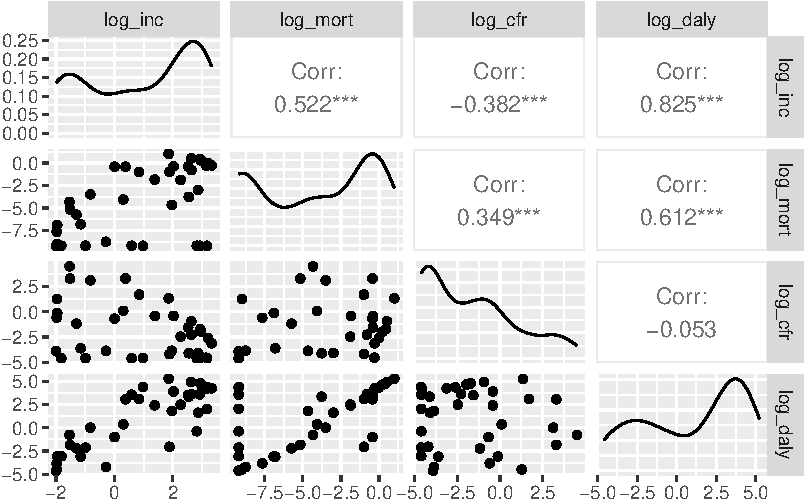
\includegraphics[keepaspectratio]{RR_TechApp_files/figure-pdf/fig-mcol-1.pdf}}

}

\caption{\label{fig-mcol}Correlation between disease burden metrics}

\end{figure}%

The final model included the rank in round 1 and log10 mortality as the
strongest predictors and an interaction term between these variables
(Table~\ref{tbl-multi}). If Rank1 was Low, the odds of Rank2 being Low
(vs.~Medium or High) was 105 times higher than if Rank1 was Medium or
High. For every unit increase in log mortality, the odds of Rank2 being
Low (vs.~Medium or High) decreased by 52\%.

\begin{Shaded}
\begin{Highlighting}[]
\NormalTok{tbl\_multi }\OtherTok{\textless{}{-}}\NormalTok{ tbl\_multi }\SpecialCharTok{\%\textgreater{}\%} 
  \FunctionTok{gt}\NormalTok{(}\AttributeTok{rowname\_col =} \StringTok{"vars"}\NormalTok{)  }\SpecialCharTok{\%\textgreater{}\%} 
   \FunctionTok{tab\_stubhead}\NormalTok{(}\AttributeTok{label =} \StringTok{"Variable"}\NormalTok{) }\SpecialCharTok{\%\textgreater{}\%} 
  \FunctionTok{tab\_spanner}\NormalTok{(}
    \AttributeTok{label =} \StringTok{"Odds ratio"}\NormalTok{,}
    \AttributeTok{columns =} \FunctionTok{c}\NormalTok{(}\StringTok{"OR"}\NormalTok{,}\StringTok{"2.5\%"}\NormalTok{, }\StringTok{"97.5\%"}\NormalTok{)) }\SpecialCharTok{\%\textgreater{}\%} 
  \FunctionTok{cols\_label}\NormalTok{(}
    \AttributeTok{OR =} \StringTok{"Median"}\NormalTok{,}
    \StringTok{"2.5\%"} \OtherTok{=} \StringTok{"2.5\%"}\NormalTok{,}
    \StringTok{"97.5\%"} \OtherTok{=} \StringTok{"97.5\%"}
\NormalTok{  ) }\SpecialCharTok{\%\textgreater{}\%} 
  \FunctionTok{tab\_options}\NormalTok{(}
    \AttributeTok{table.font.style =} \FunctionTok{px}\NormalTok{(}\DecValTok{10}\NormalTok{),}
    \AttributeTok{table.font.names =} \StringTok{"Garamond"}
\NormalTok{  )}

\NormalTok{tbl\_multi}
\end{Highlighting}
\end{Shaded}

\begin{table}

\caption{\label{tbl-multi}Multivariate analysis for round 2 rank}

\centering{

\fontsize{12.0pt}{14.4pt}\selectfont
\begin{tabular*}{\linewidth}{@{\extracolsep{\fill}}l|rrr}
\toprule
 & \multicolumn{3}{c}{Odds ratio} \\ 
\cmidrule(lr){2-4}
Variable & Median & 2.5\% & 97.5\% \\ 
\midrule\addlinespace[2.5pt]
rank1Medium & 4.913263 & 1.5910469 & 16.0600742 \\ 
rank1Low & 105.352138 & 10.6810331 & 1245.9507300 \\ 
log\_mort & 0.478776 & 0.3606483 & 0.6020927 \\ 
rank1Medium:log\_mort & 1.399504 & 1.0639050 & 1.8998095 \\ 
rank1Low:log\_mort & 1.677238 & 1.1682069 & 2.4689701 \\ 
\bottomrule
\end{tabular*}

}

\end{table}%

The interaction between the two predictors is shown in
Figure~\ref{fig-olr-int}. The top row of the figure suggests that the
probability of Rank2 being Low increases if Rank1 moves from High to Low
and decreases with increasing log mortality. The probability of Rank2
being High decreases if Rank1 moves from High to Low and increases with
increasing log mortality (bottom row of the figure). The probability of
Rank2 being Medium is independent of Rank1 and there is no monotonous
trend with log mortality. Note that the effect of log mortality on Rank2
is strong. For example, the upper right pane in the plot shows that the
probability of Rank 2 being Low if Rank 1 is Low, decreases from
approximately 60\% to almost 0\% if log mortality increases from -8 to
0. Likewise, if Rank1 is High, the probability of Rank2 being High
increases from approx. 0\% to approx. 80\% if log mortality increases
from -8 to 0.

\begin{Shaded}
\begin{Highlighting}[]
\DocumentationTok{\#\# Plotting the effects}
\CommentTok{\# https://www.r{-}bloggers.com/2019/06/how{-}to{-}perform{-}ordinal{-}logistic{-}regression{-}in{-}r/}

\NormalTok{(olr\_plot }\OtherTok{\textless{}{-}} \FunctionTok{plot}\NormalTok{(}\FunctionTok{Effect}\NormalTok{(}\AttributeTok{focal.predictors =} \FunctionTok{c}\NormalTok{(}\StringTok{"rank1"}\NormalTok{, }\StringTok{"log\_mort"}\NormalTok{),rr\_mod), }\AttributeTok{main =} \StringTok{""}\NormalTok{))}
\end{Highlighting}
\end{Shaded}

\begin{figure}[H]

\centering{

\pandocbounded{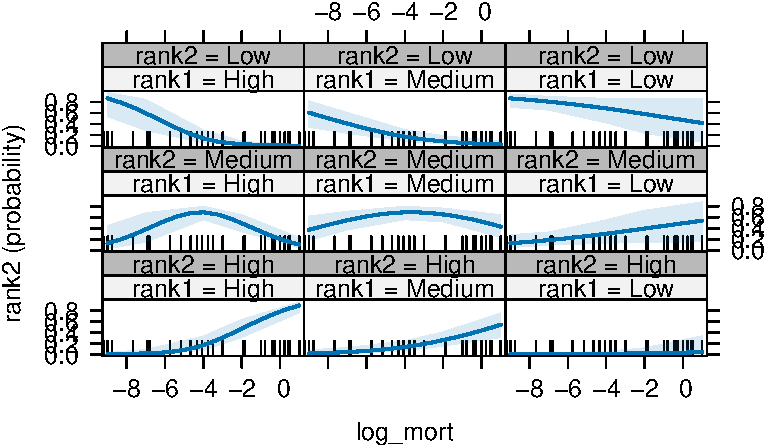
\includegraphics[keepaspectratio]{RR_TechApp_files/figure-pdf/fig-olr-int-1.pdf}}

}

\caption{\label{fig-olr-int}Interaction between predictors of rank in
round 2}

\end{figure}%

\section{Attribution of foodborne deaths to
hazards}\label{attribution-of-foodborne-deaths-to-hazards}

\subsection{The Delphi method}\label{the-delphi-method}

We used a Delphi process to collect information from Ethiopian experts
on attribution of foodborne deaths to food groups. The Delphi method is
a structured, interactive technique to elicit information from a panel
of experts and aims to move towards consensus about the study objective.
To this purpose, experts answered questions in two rounds.

\begin{itemize}
\item
  In Round 1, experts individually provided estimates of the proportion
  of illness from a given hazard, attributed to different food groups
  after having been briefed in a webinar about the specific goals of the
  study and how to complete the elicitation instrument.
\item
  After the first round, the experts received a summary of all the
  expert estimates and the rationale that was provided to support these
  estimates.
\item
  In Round 2, the experts were provided the opportunity to revise their
  individual estimates in the light of the group results.
\item
  Results from Round 2 were summarized and used to present data on the
  impact of foodborne disease by hazard and food group to the risk
  prioritization workshop.
\end{itemize}

\subsection{Round 1}\label{round-1}

\subsubsection{Elicitation instrument}\label{elicitation-instrument}

Experts were provided a spreadsheet to complete their attribution
estimates, see Figure~\ref{fig-instrument}. In addition to the sheet
shown here, there was also a sheet with free text fields for each
hazard, in which the experts could provide the rationale for their
estimates.

\begin{figure}

\centering{

\pandocbounded{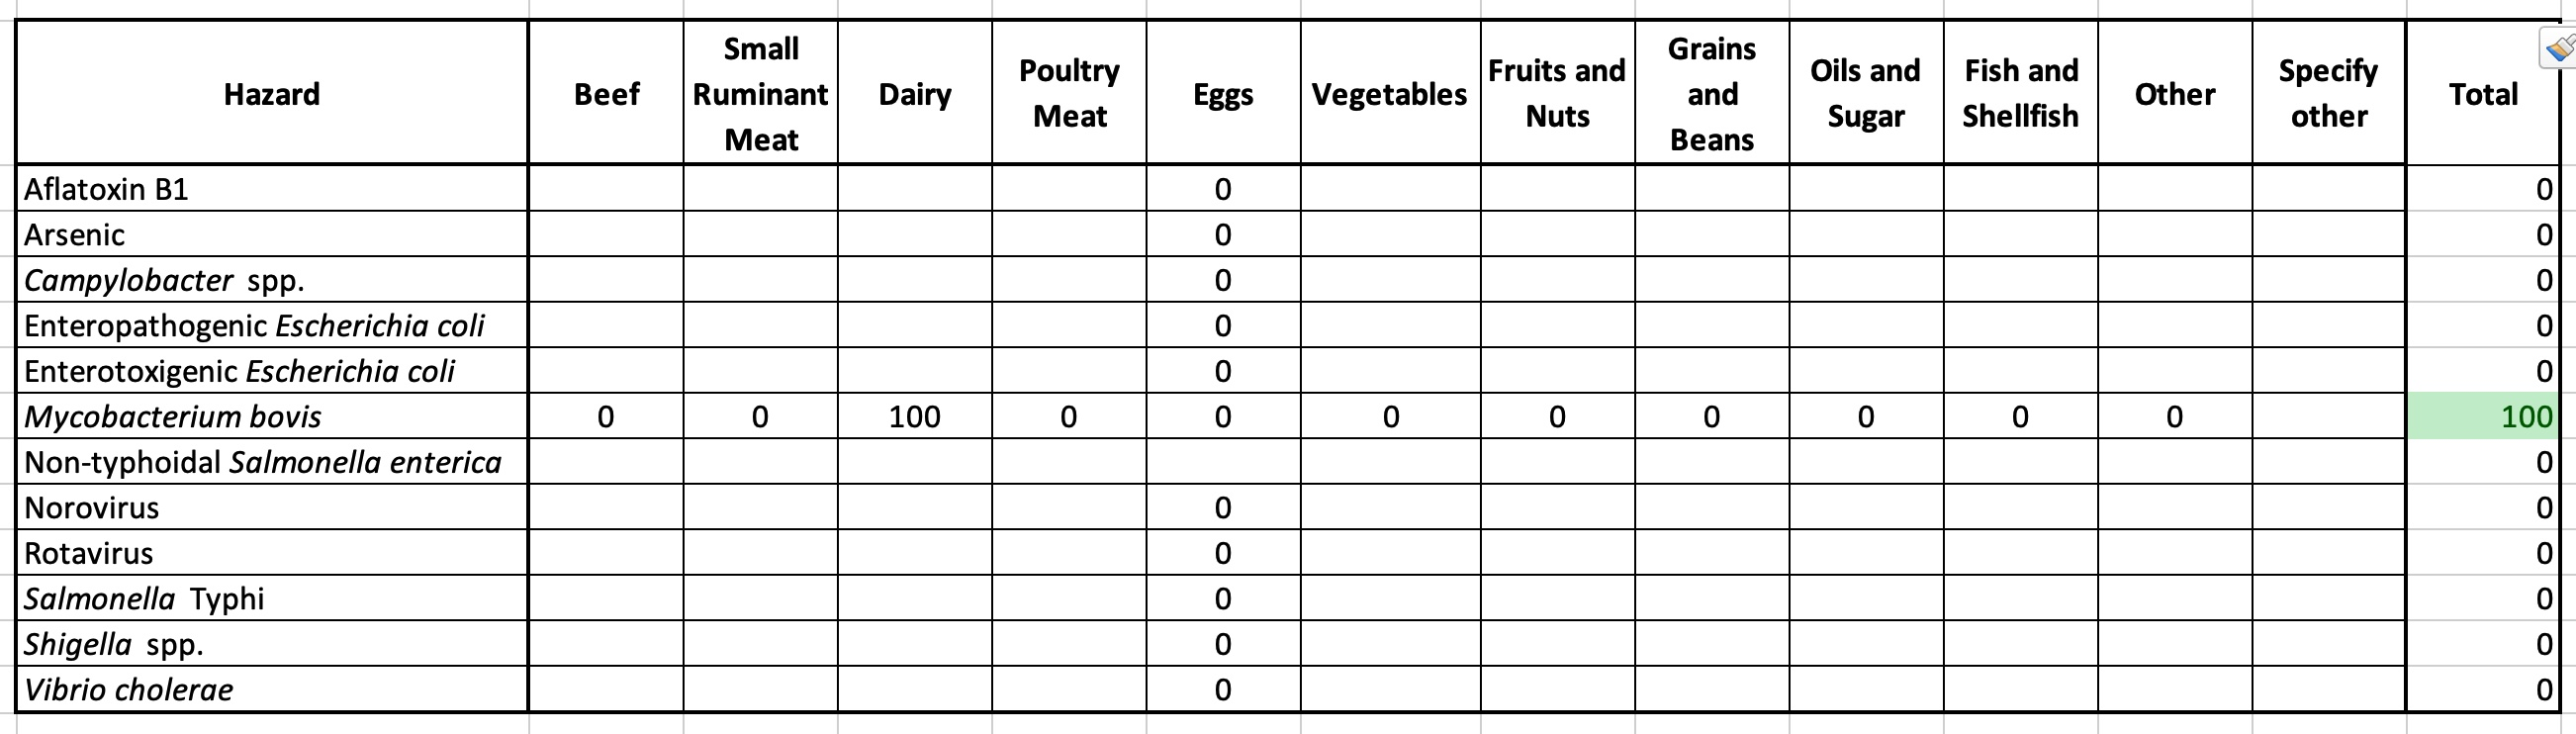
\includegraphics[keepaspectratio]{expert_instrument.jpg}}

}

\caption{\label{fig-instrument}Elicitation instrument}

\end{figure}%

The instructions to complete the elicitation instrument were:

\begin{itemize}
\item
  The aim of this exercise is to attribute all cases of \emph{foodborne
  disease} by 12 \emph{hazards}~ that were assigned a high priority in
  the risk ranking workshop in a \emph{typical year} in Ethiopia to
  \emph{food groups}.
\item
  \emph{Foodborne disease} is defined as a case of illness that was
  caused by exposure to a microbial or chemical hazard in food. Many of
  these hazards can also be transmitted by other pathways such as water,
  soil or contact with humans or animals. The data on foodborne illness
  that will be used in the study have already considered this
  attribution to major pathways.
\item
  The \emph{point of attribution} will be the point where the hazards
  entered the place where the foods are prepared for final consumption.
  Hence, experts are asked to consider both the risk of direct
  consumption of the food group as well as the risk of
  cross-contamination from the specified food group to the home kitchen
  environment or food preparation area and ready-to-eat foods prepared
  there. For example, attribution of \emph{Campylobacter} to the food
  group ``Poultry meat'' includes the risks of eating (undercooked)
  poultry meat as well as the risks of salads and other ready-to-eat
  foods that may have been contaminated through cutting boards,
  benchtops, knives, hands etc.
\item
  A \emph{typical year} is defined as a year in which no major incidents
  (e.g., a large outbreak but also COVID-19) affected the incidence of
  foodborne dise\textbf{a}se.
\item
  \emph{Food groups} included in the study are based on the WHO study,
  using 13 groups: beef, small ruminant's meat, dairy, pig's meat,
  poultry meat, eggs, vegetables, fruit and nuts, grains and beans, oils
  and sugars, finfish, shellfish, seaweed. Pork consumption is very low
  in Ethiopia and has been excluded. Eggs are not likely to be a
  relevant transmission pathway of any of the hazards except
  non-typhoidal \emph{Salmonella enterica}. Consumption of fish,
  shellfish and seaweed is low to absent in Ethiopia and are excluded.
  Attribution to oils and sugars in Africa is very low and this group
  has also been excluded. A category ``other foods'' is included to
  allow experts to name any food groups they may consider relevant,
  including those removed by the study team.
\item
  Consider all cases in the country, regardless of age, residence etc.
\item
  Start by thinking about a hazard that you are familiar with. Ask
  yourself, how are \ul{foodborne} cases by that hazard distributed
  across food groups in a typical year.
\item
  For food groups of which you think not at all involved in the
  transmission of the hazard, enter 0 in the cell for the combination of
  that hazard and food group. For example, \emph{Mycobacterium bovis}
  can only be transmitted by dairy. We have already assigned 0 to all
  food groups except dairy in the spreadsheet. We have also assigned 0
  to eggs for transmission of all hazards except \emph{Salmonella.}
  Then, consider food groups that you think are involved in transmission
  of a hazard and rank them from high to low. Distribute 100 percentage
  points over these food groups, according to your belief how important
  each food group is. If you believe a hazard is transmitted by food
  groups that are not included in the table, you can assign points to
  the group ``Other''. In that case, please specify the food in the next
  column.
\item
  The sum of all points that you assign should be 100. You can check
  this in the column ``Total'', the cells will have a green color when
  the sum is 100.
\item
  In this study, we only seek your best estimate and do not consider the
  uncertainty of these estimates.
\item
  Once you have finalized your estimates for a specific hazard, briefly
  describe your rationale in the sheet ``Rationale''. Write your
  rationale in the preassigned cell in the sheet only; the text can be
  longer than the width of the cell provided.
\item
  Repeat this process or all other hazards
\item
  You may decide that you are not sufficiently familiar with one or more
  hazards to provide estimates. In that case, leave all cells for that
  hazard blank.
\item
  Save the spreadsheet with the file name Exp\emph{xx}.xlsx, where
  \emph{xx} is the expert number that was communicated to you in the
  invitation email. This number is only known to one person in the Ohio
  State University Global One Health Initiative who is not involved in
  the study and serves to protect your anonymity.
\end{itemize}

\subsubsection{Data}\label{data-1}

Completed spreadsheets were received from 15 experts.
Table~\ref{tbl-adj} provides details on adjustments made to expert
sheets in Round1. These edits were necessary to assure consistency
between the individual expert estimates and to assure the data would fit
in the computational framework.

\begin{enumerate}
\def\labelenumi{\arabic{enumi}.}
\item
  A draft expert sheet was distributed with the invitation for the
  webinar on May 25, 2023 providing details of the process. This draft
  was revised based on feedback received from the experts. The final
  expert sheet was distributed after this webinar. Several experts used
  the draft format. Their sheets were reformatted to be consistent with
  the final format by sorting the hazards alphabetically, adding the
  food groups ``Oils and Sugar'' and ``Fish and Shellfish'', and adding
  the hazard ``Rotavirus''.
\item
  Several experts only filled cells in their spreadsheet for food groups
  to which transmission of a hazard was attributed. For computational
  purposes, empty cells for these hazards were filled with 0's.
\item
  The column ``Details'' summarized edits that were unique to individual
  expert sheets.
\end{enumerate}

\begin{Shaded}
\begin{Highlighting}[]
\NormalTok{explist1 }\OtherTok{\textless{}{-}} \FunctionTok{readRDS}\NormalTok{(}\StringTok{"explist1.rds"}\NormalTok{) }\CommentTok{\# expert data round 1}
\NormalTok{exp\_adj }\OtherTok{\textless{}{-}} \FunctionTok{read.csv}\NormalTok{(}\StringTok{"20230604\_expert\_sheet\_adjustments.csv"}\NormalTok{) }\CommentTok{\# adjustments by study team}
\NormalTok{explist2 }\OtherTok{\textless{}{-}} \FunctionTok{readRDS}\NormalTok{(}\StringTok{"explist2.rds"}\NormalTok{) }\CommentTok{\# expert data round 2}
\end{Highlighting}
\end{Shaded}

\begin{Shaded}
\begin{Highlighting}[]
\FunctionTok{gt}\NormalTok{(exp\_adj)}\SpecialCharTok{\%\textgreater{}\%} 
  \FunctionTok{tab\_options}\NormalTok{(}
    \AttributeTok{table.font.style =} \FunctionTok{px}\NormalTok{(}\DecValTok{7}\NormalTok{)}
\NormalTok{  )}
\end{Highlighting}
\end{Shaded}

\begin{table}

\caption{\label{tbl-adj}Adjustments to expert sheets}

\centering{

\fontsize{12.0pt}{14.4pt}\selectfont
\begin{tabular*}{\linewidth}{@{\extracolsep{\fill}}rlll}
\toprule
Expert & Format & Zeros & Details \\ 
\midrule\addlinespace[2.5pt]
2 & ✔️ & Added & Redistributed aflatoxin B1 over non-animal source foods \\ 
4 & R & Added & Expert added “Seafood”, which was available in new format;  \\ 
NA &  &  & estimates  moved to this column.  \\ 
NA &  &  & Redistributed aflatoxin B1 over non-animal source foods \\ 
5 & ✔️ & Added & S.Typhi Total was 110. Reduced all numbers by 10\%.  \\ 
NA &  &  & Redistributed aflatoxin B1 over non-animal source foods \\ 
9 & R & Added & Redistributed “Other”  \\ 
11 & ✔️ & ✔️ & Redistributed aflatoxin B1 over non-animal source foods \\ 
12 & ✔️ & Added & None \\ 
15 & ✔️ & Added & Divided all entries by 4 or 5 (Salmonella) to assure “Total” is 100 \\ 
16 & ✔️ & Added & Redistributed “Other”  \\ 
18 & ✔️ & Added & Redistributed aflatoxin B1 over non-animal source foods \\ 
19 & ✔️ & Added & Changed column heading to “Fish and Shellfish” \\ 
20 & ✔️ & ✔️ & Redistributed “Other”  \\ 
22 & R & Added & M. bovis was attributed 100\% to dairy by default.  \\ 
NA &  &  & Redistributed aflatoxin B1 over non-animal source foods \\ 
24 & ✔️ & Added & Removed three rows with hazards added by expert as not prioritized . \\ 
NA &  &  & Attributed Shigella and V. cholerae from eggsk to 0. \\ 
25 & ✔️ & ✔️ & Redistributed “Other”  \\ 
26 & R & ✔️ & Moved “Fish”estimates  moved to this column.  \\ 
NA &  &  & Changed “Vegetables” for EPEC to 10 to assure “Total” is 100.  \\ 
NA &  &  & Redistributed aflatoxin B1 over non-animal source foods \\ 
\bottomrule
\end{tabular*}

}

\end{table}%

\subsubsection{Average expert estimates}\label{average-expert-estimates}

The average of expert attribution estimates is presented in
Table~\ref{tbl-exp-avg}. For each hazard, the table presents the
percentage of cases of illness that is attributed to each of the 11 food
groups (including a group ``Other''). The attribution percentages per
hazard sum to 100\%.

\begin{Shaded}
\begin{Highlighting}[]
\FunctionTok{gt}\NormalTok{(exp\_avg\_round1) }\SpecialCharTok{\%\textgreater{}\%} 
  \FunctionTok{tab\_options}\NormalTok{(}
    \AttributeTok{table.font.style =} \FunctionTok{px}\NormalTok{(}\DecValTok{10}\NormalTok{),}
    \AttributeTok{table.font.names =} \StringTok{"Garamond"}
\NormalTok{  )}
\end{Highlighting}
\end{Shaded}

\begin{table}

\caption{\label{tbl-exp-avg}Average of expert attribution estimates in
Round 1 (\%). See full food group names in Figure 16.}

\centering{

\fontsize{12.0pt}{14.4pt}\selectfont
\begin{tabular*}{\linewidth}{@{\extracolsep{\fill}}lrrrrrrrrrrrr}
\toprule
Hazard & Bf & SR & Dy & Py & Eg & Vg & FN & GB & OS & SF & Ot & Tl \\ 
\midrule\addlinespace[2.5pt]
Aflatoxin B1 & 0 & 0 & 0 & 0 & 0 & 5 & 19 & 66 & 2 & 3 & 6 & 100 \\ 
Arsenic & 5 & 3 & 4 & 3 & 0 & 39 & 14 & 12 & 0 & 19 & 1 & 100 \\ 
Campylobacter & 14 & 9 & 24 & 40 & 3 & 2 & 2 & 0 & 0 & 5 & 1 & 100 \\ 
EPEC & 22 & 15 & 25 & 12 & 1 & 15 & 6 & 1 & 0 & 3 & 1 & 100 \\ 
ETEC & 24 & 15 & 26 & 12 & 1 & 13 & 4 & 0 & 0 & 3 & 1 & 100 \\ 
M. bovis & 0 & 0 & 100 & 0 & 0 & 0 & 0 & 0 & 0 & 0 & 0 & 100 \\ 
Norovirus & 13 & 7 & 14 & 12 & 2 & 23 & 18 & 1 & 0 & 8 & 2 & 100 \\ 
Rotavirus & 30 & 10 & 5 & 5 & 0 & 11 & 2 & 0 & 0 & 22 & 14 & 100 \\ 
S. Typhi & 19 & 15 & 15 & 21 & 4 & 13 & 3 & 0 & 0 & 3 & 6 & 100 \\ 
Salmonella & 10 & 11 & 10 & 13 & 18 & 24 & 9 & 0 & 0 & 5 & 0 & 100 \\ 
Shigella & 9 & 10 & 11 & 12 & 0 & 28 & 15 & 4 & 1 & 7 & 2 & 100 \\ 
V. cholerae & 9 & 6 & 9 & 6 & 1 & 37 & 11 & 2 & 2 & 14 & 3 & 100 \\ 
\bottomrule
\end{tabular*}

}

\end{table}%

\subsection{Expert agreement}\label{expert-agreement}

Table~\ref{tbl-sd} shows a metric for the (dis)agreement between
experts, i.e., the standard deviation of the estimates (in percent) for
each food-hazard pair. A zero in the table means that there was full
agreement among the experts, the higher the value, the more
disagreement. The final column in Table~\ref{tbl-sd} shows the average
standard deviation across each row, i.e., for each hazard. We note the
the experts agreed most on ETEC and least on Rotavirus. For food groups,
experts agreed most on OS and least on Vg. Note that \emph{Mycobacterium
bovis} was excluded from these considerations because it was assigned
100\% to dairy by the study team.

\begin{Shaded}
\begin{Highlighting}[]
\FunctionTok{gt}\NormalTok{(sd\_all)}\SpecialCharTok{\%\textgreater{}\%} 
  \FunctionTok{tab\_options}\NormalTok{(}
    \AttributeTok{table.font.style =} \FunctionTok{px}\NormalTok{(}\DecValTok{10}\NormalTok{),}
    \AttributeTok{table.font.names =} \StringTok{"Garamond"}
\NormalTok{  )}
\end{Highlighting}
\end{Shaded}

\begin{table}

\caption{\label{tbl-sd}Standard deviation of expert attribution
estimates in Round 1 (\%)}

\centering{

\fontsize{12.0pt}{14.4pt}\selectfont
\begin{tabular*}{\linewidth}{@{\extracolsep{\fill}}crrrrrrrrrrrr}
\toprule
Hazard & Bf & SR & Dy & Py & Eg & Vg & FN & GB & OS & SF & Ot & Average \\ 
\midrule\addlinespace[2.5pt]
Aflatoxin B1 & 0 & 0 & 0 & 0 & 0 & 9 & 17 & 27 & 4 & 9 & 10 & 7 \\ 
Arsenic & 9 & 7 & 8 & 6 & 0 & 23 & 17 & 16 & 0 & 24 & 3 & 10 \\ 
Campylobacter & 10 & 8 & 16 & 24 & 8 & 3 & 3 & 1 & 0 & 10 & 4 & 8 \\ 
EPEC & 10 & 12 & 9 & 9 & 3 & 14 & 7 & 3 & 0 & 6 & 3 & 7 \\ 
ETEC & 7 & 11 & 14 & 9 & 3 & 11 & 5 & 1 & 0 & 6 & 2 & 6 \\ 
M. bovis & 0 & 0 & 0 & 0 & 0 & 0 & 0 & 0 & 0 & 0 & 0 & 0 \\ 
Norovirus & 11 & 10 & 11 & 13 & 4 & 21 & 19 & 2 & 0 & 11 & 4 & 10 \\ 
Rotavirus & 48 & 12 & 10 & 10 & 0 & 13 & 5 & 0 & 0 & 21 & 16 & 12 \\ 
S. Typhi & 9 & 11 & 10 & 12 & 8 & 11 & 4 & 1 & 1 & 5 & 11 & 8 \\ 
Salmonella & 10 & 14 & 10 & 11 & 26 & 24 & 13 & 1 & 1 & 13 & 1 & 11 \\ 
Shigella & 8 & 12 & 8 & 17 & 0 & 19 & 15 & 6 & 3 & 10 & 5 & 9 \\ 
V. cholerae & 12 & 10 & 9 & 9 & 3 & 31 & 9 & 4 & 4 & 27 & 8 & 11 \\ 
NA & 11 & 9 & 9 & 10 & 5 & 15 & 9 & 5 & 1 & 12 & 6 & 8 \\ 
\bottomrule
\end{tabular*}

}

\end{table}%

\subsection{Expert rationale}\label{expert-rationale}

Experts were asked to provide the rationale for their estimates, and
these are reproduced \emph{ad verbatim} in @-tbl-rat (Appendix A). This
information was shared to help other experts evaluate the group
consensus and decide whether they wanted to adjust their estimates in
Round 2.

\subsection{Evaluation Round 1}\label{evaluation-round-1}

After considering the expert's estimates and rationale, the TARTARE team
provided the following observations for consideration by the experts in
round 2.

\begin{enumerate}
\def\labelenumi{\arabic{enumi}.}
\item
  Aflatoxin B1 only occurs in foods of plant origin, mainly tree nuts
  and grains and oil seeds. It can also be present in animal feed.
  However, after ingestion by animals, aflatoxin B1 is converted into
  aflatoxin M1 and excreted in urine and milk. Aflatoxin B1 does
  \ul{not} occur in meat and dairy. Aflatoxin M1 was included in the
  risk ranking workshop and was not considered a high priority foodborne
  hazard.
\item
  Arsenic occurs naturally in soils and can be accumulated by plants
  grown in contaminated soils. Imported rice is an important, but
  under-recognized source of exposure to arsenic in Africa. Fish mainly
  contains arsenobetain (the least toxic form of arsenic), rice, which
  contains primarily inorganic arsenic, which is much more toxic (L. van
  Ingenbleek, WHO, personal communication).
\item
  Enteropathogenic and enterotoxigenic \emph{E. coli}, Norovirus,
  Rotavirus, \emph{Salmonella} Typhi and \emph{Shigella} spp. have
  exclusively human reservoirs. The reservoirs of \emph{Vibrio cholerae}
  are humans and water. Cross-contamination from food handlers to animal
  source foods is possible, and Ethiopian experts have indicated that
  meat and dairy may be involved in the transmission of these hazards
  (\emph{7}). However, it is unlikely that animal source foods are their
  main transmission routes.
\item
  Some experts mentioned the importance of water as a transmission
  route. There is no doubt that waterborne transmission contributes
  significantly to the spread of many hazards considered in this study.
  However, the differentiation between food- and waterborne exposure is
  already accounted for in the WHO FERG estimates and the attribution
  estimated from this study will be applied to estimates of the
  \ul{foodborne} disease burden only. Experts should therefore not
  consider waterborne transmission in their estimates.
\end{enumerate}

\subsection{Round 2}\label{round-2}

\subsubsection{Instructions}\label{instructions}

All experts were invited to review the changes made to their worksheets
by the study team and adjust their Round 2 estimates if they disagreed
with any of the edits. Experts who used the draft format did not
consider attribution of ``Rotavirus'' nor the newly added food groups
and were invited to reconsider their estimates in Round 2 to take these
changes into account.

Experts were also invited to review the Round 1 group results and the
comments from the study team and, if they wished, change their estimates
based on this information.

If they did not want to make any changes, they were asked to confirm by
reply email. After a set deadline, the study team assumed Round 1
estimates were still valid.

\subsubsection{Data}\label{data-2}

In Round 2, three experts provided revised estimates. For all other
experts, the Round 1 estimates were considered final.

\subsubsection{Updated expert estimates}\label{updated-expert-estimates}

Updated expert estimates are provided in Table~\ref{tbl-exp-avg2}.
Because of the low number of revised estimates, the results are quite
similar to those in Round 1.

\begin{Shaded}
\begin{Highlighting}[]
\FunctionTok{gt}\NormalTok{(exp\_avg\_round2) }\SpecialCharTok{\%\textgreater{}\%} 
  \FunctionTok{tab\_options}\NormalTok{(}
    \AttributeTok{table.font.style =} \FunctionTok{px}\NormalTok{(}\DecValTok{10}\NormalTok{),}
    \AttributeTok{table.font.names =} \StringTok{"Garamond"}
\NormalTok{  )}
\end{Highlighting}
\end{Shaded}

\begin{table}

\caption{\label{tbl-exp-avg2}Average of expert attribution estimates in
Round 2(\%)}

\centering{

\fontsize{12.0pt}{14.4pt}\selectfont
\begin{tabular*}{\linewidth}{@{\extracolsep{\fill}}lrrrrrrrrrrrr}
\toprule
Hazard & Bf & SR & Dy & Py & Eg & Vg & FN & GB & OS & SF & Ot & Tl \\ 
\midrule\addlinespace[2.5pt]
Aflatoxin B1 & 0 & 0 & 0 & 0 & 0 & 6 & 20 & 67 & 1 & 2 & 5 & 100 \\ 
Arsenic & 4 & 2 & 3 & 2 & 0 & 39 & 14 & 15 & 0 & 20 & 1 & 100 \\ 
Campylobacter & 14 & 9 & 23 & 40 & 3 & 3 & 2 & 0 & 0 & 5 & 1 & 100 \\ 
EPEC & 22 & 15 & 25 & 12 & 1 & 15 & 6 & 1 & 0 & 3 & 2 & 100 \\ 
ETEC & 24 & 15 & 26 & 12 & 1 & 13 & 4 & 0 & 0 & 3 & 1 & 100 \\ 
M. bovis & 0 & 0 & 100 & 0 & 0 & 0 & 0 & 0 & 0 & 0 & 0 & 100 \\ 
Norovirus & 14 & 8 & 16 & 13 & 2 & 22 & 16 & 1 & 0 & 7 & 2 & 100 \\ 
Rotavirus & 27 & 9 & 6 & 4 & 0 & 15 & 6 & 0 & 0 & 22 & 11 & 100 \\ 
S. Typhi & 19 & 15 & 15 & 21 & 4 & 13 & 3 & 0 & 0 & 3 & 6 & 100 \\ 
Salmonella & 10 & 11 & 12 & 12 & 17 & 23 & 9 & 0 & 0 & 5 & 1 & 100 \\ 
Shigella & 9 & 10 & 11 & 13 & 0 & 28 & 15 & 3 & 1 & 7 & 2 & 100 \\ 
V. cholerae & 10 & 6 & 10 & 6 & 1 & 37 & 10 & 2 & 2 & 14 & 3 & 100 \\ 
\bottomrule
\end{tabular*}

}

\end{table}%

\subsection{Attribution to food
groups}\label{attribution-to-food-groups}

In the risk ranking workshop, the experts indicated that mortality was
the main metric considered in hazard ranking. This was also evident from
the analysis presented in Table~\ref{tbl-multi}. Therefore, data on
deaths per hazard/ food group were presented as the key input in the
risk prioritization workshop. Note that attribution of foodborne deaths
was assumed to be proportional to attribution of foodborne disease
cases. In total, \ensuremath{1.48077\times 10^{5}} deaths were estimated
to have occurred in 2010 due to foodborne disease in Ethiopia. The
proportion of cases attributed by FERG to different food/hazard
combinations for the AFRE subregion, to which Ethiopia belongs, is shown
in Table~\ref{tbl-prior-attr}. These estimates are the average for the
subregion, and were updated for Ethiopia using the results from the
Delphi survey.

FERG has not presented attribution estimates to food groups for
pathogens with human reservoirs (ETEC, EPEC, \emph{Shigella} spp.,
Norovirus) and arsenic. Estimates for ETEC were available for Ethiopia
from an expert elicitation for the TARTARE and Pull Push projects
(\emph{7}). It was assumed that attribution for other pathogens with
human reservoirs was the same as for ETEC. In Africa, fish and rice
(mainly imported rice) are the main sources of foodborne exposure to
arsenic (Luc van Inglenbeek, WHO; personal communication). A less toxic
form of arsenic occurs in fish than in rice. Hence 90\% of all deaths by
arsenic were attributed to the food group ``Grains\_Beans'' and 10\% to
``(Shell)fish''.

\begin{Shaded}
\begin{Highlighting}[]
\FunctionTok{gt}\NormalTok{(attr\_prior) }\SpecialCharTok{\%\textgreater{}\%} 
  \FunctionTok{tab\_options}\NormalTok{(}
    \AttributeTok{table.font.style =} \FunctionTok{px}\NormalTok{(}\DecValTok{10}\NormalTok{),}
    \AttributeTok{table.font.names =} \StringTok{"Garamond"}
\NormalTok{  )}
\end{Highlighting}
\end{Shaded}

\begin{table}

\caption{\label{tbl-prior-attr}Prior attribution estimates (percent)}

\centering{

\fontsize{12.0pt}{14.4pt}\selectfont
\begin{tabular*}{\linewidth}{@{\extracolsep{\fill}}lrrrrrrrrrrrr}
\toprule
Hazard & Bf & SR & Dy & Py & Eg & Vg & FN & GB & OS & SF & Ot & Tl \\ 
\midrule\addlinespace[2.5pt]
Aflatoxin B1 & 0 & 0 & 0 & 0 & 0 & 0 & 50 & 50 & 0 & 0 & 0 & 100 \\ 
Arsenic & 0 & 0 & 0 & 0 & 0 & 0 & 0 & 90 & 0 & 10 & 0 & 100 \\ 
Campylobacter & 12 & 12 & 15 & 51 & 0 & 8 & 2 & 0 & 0 & 0 & 0 & 100 \\ 
EPEC & 13 & 9 & 24 & 21 & 0 & 19 & 7 & 3 & 3 & 1 & 0 & 100 \\ 
ETEC & 13 & 9 & 24 & 21 & 0 & 19 & 7 & 3 & 3 & 1 & 0 & 100 \\ 
M. bovis & 0 & 0 & 100 & 0 & 0 & 0 & 0 & 0 & 0 & 0 & 0 & 100 \\ 
Norovirus & 8 & 8 & 7 & 35 & 23 & 7 & 6 & 2 & 1 & 2 & 2 & 101 \\ 
Rotavirus & 13 & 9 & 24 & 21 & 0 & 19 & 7 & 3 & 3 & 1 & 0 & 100 \\ 
S. Typhi & 13 & 9 & 24 & 21 & 0 & 19 & 7 & 3 & 3 & 1 & 0 & 100 \\ 
Salmonella & 13 & 9 & 24 & 21 & 0 & 19 & 7 & 3 & 3 & 1 & 0 & 100 \\ 
Shigella & 13 & 9 & 24 & 21 & 0 & 19 & 7 & 3 & 3 & 1 & 0 & 100 \\ 
V. cholerae & 13 & 9 & 24 & 21 & 0 & 19 & 7 & 3 & 3 & 1 & 0 & 100 \\ 
\bottomrule
\end{tabular*}

}

\end{table}%

We updated the prior attribution data using the data provided by the
experts by calculating a weighted average. Let \(a_{ij}\) be the prior
estimates of percentage points of deaths by hazard \(i\) assigned to
food group \(j\), and \(b_{ijk}\) be the percentage points of deaths by
hazard \(i\) assigned to food group \(j\) by expert \(k\). An equal
weights average was chosen to combine the prior estmates and expert's
inputs:

\[ \mu_{ij}=\frac{a_{ij}+\sum_{k} (b_{ijk}/k)}{2}\]

\begin{Shaded}
\begin{Highlighting}[]
\FunctionTok{gt}\NormalTok{(attr\_post) }\SpecialCharTok{\%\textgreater{}\%} 
  \FunctionTok{tab\_options}\NormalTok{(}
    \AttributeTok{table.font.style =} \FunctionTok{px}\NormalTok{(}\DecValTok{10}\NormalTok{),}
    \AttributeTok{table.font.names =} \StringTok{"Garamond"}
\NormalTok{  )}
\end{Highlighting}
\end{Shaded}

\begin{table}

\caption{\label{tbl-post-attr}Posterior attribution combining estimates
from experts in Ethiopia and from FERG}

\centering{

\fontsize{12.0pt}{14.4pt}\selectfont
\begin{tabular*}{\linewidth}{@{\extracolsep{\fill}}lrrrrrrrrrrrr}
\toprule
Hazard & Bf & SR & Dy & Py & Eg & Vg & FN & GB & OS & SF & Ot & Tl \\ 
\midrule\addlinespace[2.5pt]
Aflatoxin B1 & 0 & 0 & 0 & 0 & 0 & 3 & 35 & 58 & 0 & 1 & 2 & 100 \\ 
Arsenic & 2 & 1 & 2 & 1 & 0 & 19 & 7 & 52 & 0 & 15 & 0 & 100 \\ 
Campylobacter & 13 & 11 & 19 & 46 & 2 & 5 & 2 & 0 & 0 & 3 & 1 & 100 \\ 
EPEC & 17 & 12 & 24 & 16 & 0 & 17 & 6 & 2 & 2 & 2 & 1 & 100 \\ 
ETEC & 19 & 12 & 25 & 17 & 0 & 16 & 6 & 2 & 2 & 2 & 1 & 100 \\ 
M. bovis & 0 & 0 & 100 & 0 & 0 & 0 & 0 & 0 & 0 & 0 & 0 & 100 \\ 
Norovirus & 11 & 8 & 11 & 24 & 13 & 14 & 11 & 1 & 0 & 5 & 2 & 100 \\ 
Rotavirus & 20 & 9 & 15 & 13 & 0 & 17 & 6 & 2 & 2 & 12 & 5 & 100 \\ 
S. Typhi & 16 & 12 & 19 & 21 & 2 & 16 & 5 & 2 & 2 & 2 & 3 & 100 \\ 
Salmonella & 12 & 10 & 18 & 16 & 8 & 21 & 8 & 2 & 2 & 3 & 0 & 100 \\ 
Shigella & 11 & 10 & 17 & 17 & 0 & 24 & 11 & 3 & 2 & 4 & 1 & 100 \\ 
V. cholerae & 11 & 8 & 17 & 14 & 0 & 28 & 9 & 2 & 2 & 7 & 1 & 100 \\ 
\bottomrule
\end{tabular*}

}

\end{table}%

\subsection{Updated attributable
deaths}\label{updated-attributable-deaths}

Applying the updated attribution estimates resulted in estimates of the
number of foodborne deaths attributed to each hazard/food group pair,
see Table~\ref{tbl-post-attr_deaths}.

\begin{Shaded}
\begin{Highlighting}[]
\NormalTok{attr\_deaths\_post }\OtherTok{\textless{}{-}}\NormalTok{ attr\_post[ , }\DecValTok{2}\SpecialCharTok{:}\DecValTok{12}\NormalTok{] }\SpecialCharTok{*}\NormalTok{ deaths }\SpecialCharTok{/} \DecValTok{100}
\CommentTok{\# https://www.w3schools.blog/round{-}all{-}columns{-}in{-}r{-}data frame{-}to{-}3{-}digits}

\NormalTok{attr\_deaths\_post }\OtherTok{\textless{}{-}} \FunctionTok{round}\NormalTok{(attr\_deaths\_post, }\DecValTok{0}\NormalTok{)}

\NormalTok{attr\_deaths\_post }\OtherTok{\textless{}{-}} \FunctionTok{data.frame}\NormalTok{(}\FunctionTok{cbind}\NormalTok{(attr\_prior[, }\DecValTok{1}\NormalTok{], attr\_deaths\_post)) }\SpecialCharTok{\%\textgreater{}\%} \FunctionTok{mutate}\NormalTok{(}\AttributeTok{Total =} \FunctionTok{rowSums}\NormalTok{(}\FunctionTok{across}\NormalTok{(}\FunctionTok{where}\NormalTok{(is.numeric))))}
\FunctionTok{colnames}\NormalTok{(attr\_deaths\_post) }\OtherTok{\textless{}{-}} \FunctionTok{c}\NormalTok{(}\FunctionTok{colnames}\NormalTok{(attr\_prior)[}\DecValTok{1}\SpecialCharTok{:}\DecValTok{12}\NormalTok{], }\StringTok{"Total"}\NormalTok{)}
\FunctionTok{saveRDS}\NormalTok{(attr\_deaths\_post, }\StringTok{"attr\_deaths\_post.rds"}\NormalTok{)}
\end{Highlighting}
\end{Shaded}

\begin{Shaded}
\begin{Highlighting}[]
\NormalTok{attr\_deaths\_post }\SpecialCharTok{\%\textgreater{}\%} 
  \FunctionTok{adorn\_totals}\NormalTok{() }\SpecialCharTok{\%\textgreater{}\%}
  \FunctionTok{gt}\NormalTok{() }\SpecialCharTok{\%\textgreater{}\%} 
    \FunctionTok{tab\_options}\NormalTok{(}
      \AttributeTok{table.font.style =} \FunctionTok{px}\NormalTok{(}\DecValTok{10}\NormalTok{),}
      \AttributeTok{table.font.names =} \StringTok{"Garamond"}\NormalTok{)}
\end{Highlighting}
\end{Shaded}

\begin{table}

\caption{\label{tbl-post-attr_deaths}Attributable deaths by hazard and
food group, combining attribution estimates from experts in Ethiopia and
literature}

\centering{

\fontsize{12.0pt}{14.4pt}\selectfont
\begin{tabular*}{\linewidth}{@{\extracolsep{\fill}}lrrrrrrrrrrrr}
\toprule
Hazard & Bf & SR & Dy & Py & Eg & Vg & FN & GB & OS & SF & Ot & Total \\ 
\midrule\addlinespace[2.5pt]
Aflatoxin B1 & 0 & 0 & 0 & 0 & 0 & 2 & 20 & 32 & 0 & 1 & 1 & 56 \\ 
Arsenic & 13 & 6 & 13 & 6 & 0 & 123 & 45 & 337 & 0 & 97 & 0 & 640 \\ 
Campylobacter & 86 & 73 & 125 & 304 & 13 & 33 & 13 & 0 & 0 & 20 & 7 & 674 \\ 
EPEC & 248 & 175 & 350 & 233 & 0 & 248 & 87 & 29 & 29 & 29 & 15 & 1443 \\ 
ETEC & 210 & 133 & 277 & 188 & 0 & 177 & 66 & 22 & 22 & 22 & 11 & 1128 \\ 
M. bovis & 0 & 0 & 125 & 0 & 0 & 0 & 0 & 0 & 0 & 0 & 0 & 125 \\ 
Norovirus & 148 & 108 & 148 & 324 & 175 & 189 & 148 & 13 & 0 & 67 & 27 & 1347 \\ 
Rotavirus & 173 & 78 & 130 & 113 & 0 & 147 & 52 & 17 & 17 & 104 & 43 & 874 \\ 
S. Typhi & 102 & 77 & 122 & 134 & 13 & 102 & 32 & 13 & 13 & 13 & 19 & 640 \\ 
Salmonella & 71 & 60 & 107 & 95 & 48 & 125 & 48 & 12 & 12 & 18 & 0 & 596 \\ 
Shigella & 44 & 40 & 67 & 67 & 0 & 95 & 44 & 12 & 8 & 16 & 4 & 397 \\ 
V. cholerae & 260 & 189 & 402 & 331 & 0 & 663 & 213 & 47 & 47 & 166 & 24 & 2342 \\ 
Total & 1355 & 939 & 1866 & 1795 & 249 & 1904 & 768 & 534 & 148 & 553 & 151 & 10262 \\ 
\bottomrule
\end{tabular*}

}

\end{table}%

The code below creates a data frame and two plots showing the
distribution of attributable deaths by hazard and food group. Plots are
included in the main text of the manuscript.

\begin{Shaded}
\begin{Highlighting}[]
\NormalTok{attr\_deaths\_post\_long }\OtherTok{\textless{}{-}} \FunctionTok{melt}\NormalTok{(attr\_deaths\_post)}
\FunctionTok{colnames}\NormalTok{(attr\_deaths\_post\_long) }\OtherTok{\textless{}{-}} \FunctionTok{c}\NormalTok{(}\StringTok{"Hazard"}\NormalTok{, }\StringTok{"Food\_group"}\NormalTok{, }\StringTok{"Attributable\_deaths"}\NormalTok{)}

\CommentTok{\# Remove totals}
\NormalTok{attr\_deaths\_post\_long }\OtherTok{\textless{}{-}}\NormalTok{ attr\_deaths\_post\_long }\SpecialCharTok{|\textgreater{}} 
  \FunctionTok{filter}\NormalTok{(Food\_group}\SpecialCharTok{!=} \StringTok{"Total"}\NormalTok{)}
\NormalTok{attr\_deaths\_post\_long}\SpecialCharTok{$}\NormalTok{Hazard }\OtherTok{\textless{}{-}} \FunctionTok{factor}\NormalTok{(attr\_deaths\_post\_long}\SpecialCharTok{$}\NormalTok{Hazard) }\SpecialCharTok{|\textgreater{}} 
  \FunctionTok{fct\_rev}\NormalTok{()}

\CommentTok{\# Create hazard labels with proper italics and food group labels}
\NormalTok{haz.labels }\OtherTok{\textless{}{-}} \FunctionTok{c}\NormalTok{(}\StringTok{"Aflatoxin B1"}\NormalTok{, }\StringTok{"Arsenic"}\NormalTok{, }\StringTok{"*Campylobacter* spp."}\NormalTok{,}
\StringTok{"Enteropathogenic *Escherichia coli*"}\NormalTok{, }\StringTok{"Enterotoxigenic *Escherichia coli*"}\NormalTok{,}
\StringTok{"*Mycobacterium bovis*"}\NormalTok{, }\StringTok{"Non{-}typhoidal *Salmonella enterica*"}\NormalTok{, }\StringTok{"Norovirus"}\NormalTok{,}
\StringTok{"Rotavirus"}\NormalTok{, }\StringTok{"*Salmonella* Typhi"}\NormalTok{, }\StringTok{"*Shigella* spp."}\NormalTok{, }\StringTok{"*Vibrio cholerae*"}\NormalTok{ )}
\NormalTok{fg.labels }\OtherTok{\textless{}{-}} \FunctionTok{c}\NormalTok{(}\StringTok{"Beef"}\NormalTok{, }\StringTok{"Small Ruminant Meat"}\NormalTok{, }\StringTok{"Dairy"}\NormalTok{, }\StringTok{"Poultry"}\NormalTok{, }\StringTok{"Eggs"}\NormalTok{, }\StringTok{"Vegetables"}\NormalTok{, }\StringTok{"Fruits \& Nuts"}\NormalTok{, }\StringTok{"Grains \& Beans"}\NormalTok{, }\StringTok{"Oils \& Sugar"}\NormalTok{, }\StringTok{"(Shell)fish"}\NormalTok{, }\StringTok{"Other"}\NormalTok{)}

\CommentTok{\# Palette Spectral has only 12 colors, need to extend that to 13}
\NormalTok{mySpectral }\OtherTok{\textless{}{-}} \FunctionTok{colorRampPalette}\NormalTok{(}\FunctionTok{brewer.pal}\NormalTok{(}\DecValTok{11}\NormalTok{, }\StringTok{"Spectral"}\NormalTok{))(}\DecValTok{13}\NormalTok{)}
\end{Highlighting}
\end{Shaded}

\begin{Shaded}
\begin{Highlighting}[]
\NormalTok{by\_hazard }\OtherTok{\textless{}{-}} 
  \FunctionTok{ggplot}\NormalTok{(attr\_deaths\_post\_long, }\FunctionTok{aes}\NormalTok{(}\AttributeTok{x =}\NormalTok{ Hazard, }\AttributeTok{y =}\NormalTok{ Attributable\_deaths, }\AttributeTok{fill =}\NormalTok{ Food\_group)) }\SpecialCharTok{+} 
  \FunctionTok{geom\_bar}\NormalTok{(}\AttributeTok{stat =} \StringTok{"identity"}\NormalTok{) }\SpecialCharTok{+}
  \FunctionTok{scale\_fill\_manual}\NormalTok{(}\AttributeTok{values =}\NormalTok{ mySpectral, }\AttributeTok{name =} \StringTok{"Food group"}\NormalTok{, }\AttributeTok{labels =}\NormalTok{ fg.labels) }\SpecialCharTok{+}
  \FunctionTok{ylab}\NormalTok{(}\StringTok{"Attributable deaths"}\NormalTok{) }\SpecialCharTok{+}
  \FunctionTok{theme\_classic}\NormalTok{() }\SpecialCharTok{+}
  \FunctionTok{scale\_x\_discrete}\NormalTok{(}\AttributeTok{labels =} \FunctionTok{rev}\NormalTok{(haz.labels)) }\SpecialCharTok{+}
  \FunctionTok{theme}\NormalTok{(}\AttributeTok{axis.text.y =} \FunctionTok{element\_markdown}\NormalTok{()) }\SpecialCharTok{+}
  \FunctionTok{rotate}\NormalTok{()}

\FunctionTok{ggsave}\NormalTok{(}\AttributeTok{plot =}\NormalTok{ by\_hazard, }\AttributeTok{filename =} \StringTok{"by\_hazard.tiff"}\NormalTok{)}
\end{Highlighting}
\end{Shaded}

\begin{Shaded}
\begin{Highlighting}[]
\NormalTok{by\_food\_group }\OtherTok{\textless{}{-}} 
  \FunctionTok{ggplot}\NormalTok{(attr\_deaths\_post\_long, }\FunctionTok{aes}\NormalTok{(}\AttributeTok{x =}\NormalTok{ Food\_group,}
                                    \AttributeTok{y =}\NormalTok{ Attributable\_deaths, }\AttributeTok{fill =}\NormalTok{ Hazard)) }\SpecialCharTok{+} 
  \FunctionTok{geom\_bar}\NormalTok{(}\AttributeTok{stat =} \StringTok{"identity"}\NormalTok{) }\SpecialCharTok{+}
  \FunctionTok{scale\_fill\_manual}\NormalTok{(}\AttributeTok{values =}\NormalTok{ mySpectral, }\AttributeTok{labels =} \FunctionTok{rev}\NormalTok{(haz.labels)) }\SpecialCharTok{+}
  \FunctionTok{ylab}\NormalTok{(}\StringTok{"Attributable deaths"}\NormalTok{) }\SpecialCharTok{+}
  \FunctionTok{theme\_classic}\NormalTok{() }\SpecialCharTok{+}
  \FunctionTok{scale\_x\_discrete}\NormalTok{(}\AttributeTok{name =} \StringTok{"Food group"}\NormalTok{, }\AttributeTok{labels =} \FunctionTok{rev}\NormalTok{(fg.labels), }\AttributeTok{limits =}\NormalTok{ rev) }\SpecialCharTok{+}
  \FunctionTok{theme}\NormalTok{(}\AttributeTok{axis.text.y =} \FunctionTok{element\_markdown}\NormalTok{(),}
        \AttributeTok{fill =} \FunctionTok{element\_markdown}\NormalTok{()) }\SpecialCharTok{+}
  \FunctionTok{theme}\NormalTok{(}\AttributeTok{legend.text =} \FunctionTok{element\_markdown}\NormalTok{()) }\SpecialCharTok{+}
  \FunctionTok{theme}\NormalTok{(}\AttributeTok{legend.key.height=} \FunctionTok{unit}\NormalTok{(.}\DecValTok{5}\NormalTok{, }\StringTok{\textquotesingle{}cm\textquotesingle{}}\NormalTok{),}
        \AttributeTok{legend.key.width=} \FunctionTok{unit}\NormalTok{(.}\DecValTok{25}\NormalTok{, }\StringTok{\textquotesingle{}cm\textquotesingle{}}\NormalTok{)) }\SpecialCharTok{+}
  \FunctionTok{rotate}\NormalTok{()}

\FunctionTok{ggsave}\NormalTok{(}\AttributeTok{plot =}\NormalTok{ by\_food\_group, }\AttributeTok{filename =} \StringTok{"by\_food\_group.tiff"}\NormalTok{)}
\end{Highlighting}
\end{Shaded}

\section{Prioritization}\label{prioritization}

\subsection{Foodborne deaths attributable to Supply Chain Control Points
in four food value
chains}\label{foodborne-deaths-attributable-to-supply-chain-control-points-in-four-food-value-chains}

The code in this section aggregates the attributable deaths to three
categories of hazards and creates the number of deaths for each
combination of hazards and food groups.

\begin{Shaded}
\begin{Highlighting}[]
\NormalTok{deaths\_fg }\OtherTok{\textless{}{-}} \FunctionTok{readRDS}\NormalTok{(}\StringTok{"attr\_deaths\_post.rds"}\NormalTok{)}
\FunctionTok{colnames}\NormalTok{(deaths\_fg) }\OtherTok{\textless{}{-}} \FunctionTok{c}\NormalTok{(}\StringTok{"hazard"}\NormalTok{, }\StringTok{"beef"}\NormalTok{, }\StringTok{"small\_ruminant\_meat"}\NormalTok{, }\StringTok{"dairy"}\NormalTok{, }\StringTok{"poultry\_meat"}\NormalTok{,}\StringTok{"eggs"}\NormalTok{, }\StringTok{"vegetables"}\NormalTok{, }\StringTok{"fruits\_nuts"}\NormalTok{, }\StringTok{"grains\_beans"}\NormalTok{, }\StringTok{"oils\_sugar"}\NormalTok{, }\StringTok{"fish\_shellfish"}\NormalTok{, }\StringTok{"other"}\NormalTok{, }\StringTok{"total"}\NormalTok{)}

\NormalTok{deaths\_fg }\OtherTok{\textless{}{-}}\NormalTok{ deaths\_fg }\SpecialCharTok{\%\textgreater{}\%} 
  \FunctionTok{mutate}\NormalTok{(}\AttributeTok{drm =}\NormalTok{ beef }\SpecialCharTok{+}\NormalTok{ small\_ruminant\_meat,}
         \AttributeTok{ddr =}\NormalTok{ dairy,}
         \AttributeTok{dpl =}\NormalTok{ poultry\_meat }\SpecialCharTok{+}\NormalTok{ eggs,}
         \AttributeTok{dvg =}\NormalTok{ vegetables,}
         \AttributeTok{source =} \FunctionTok{factor}\NormalTok{(}\FunctionTok{c}\NormalTok{(}\StringTok{"chem"}\NormalTok{, }\StringTok{"chem"}\NormalTok{, }\StringTok{"zoon"}\NormalTok{, }\StringTok{"anthro"}\NormalTok{,}
                           \StringTok{"anthro"}\NormalTok{,}\StringTok{"zoon"}\NormalTok{, }\StringTok{"zoon"}\NormalTok{,}
                           \FunctionTok{rep}\NormalTok{(}\StringTok{"anthro"}\NormalTok{, }\DecValTok{5}\NormalTok{)),}
                    \AttributeTok{levels =} \FunctionTok{c}\NormalTok{(}\StringTok{"anthro"}\NormalTok{, }\StringTok{"zoon"}\NormalTok{, }\StringTok{"chem"}\NormalTok{))}
\NormalTok{         ) }\SpecialCharTok{\%\textgreater{}\%} 
\NormalTok{   dplyr}\SpecialCharTok{::}\FunctionTok{select}\NormalTok{(hazard, drm, ddr, dpl, dvg, source)}

\NormalTok{deaths\_agg }\OtherTok{\textless{}{-}} \FunctionTok{aggregate}\NormalTok{(}\FunctionTok{cbind}\NormalTok{(drm, ddr, dpl, dvg) }\SpecialCharTok{\textasciitilde{}}\NormalTok{ source, }\AttributeTok{data=}\NormalTok{deaths\_fg, sum) }\SpecialCharTok{\%\textgreater{}\%} 
  \FunctionTok{adorn\_totals}\NormalTok{(}\StringTok{"row"}\NormalTok{)}

\CommentTok{\# Transpose data frame}
\CommentTok{\# https://kphahn57.medium.com/peters{-}r{-}transpose{-}a{-}tibble{-}92536a24ff3b}

\NormalTok{deaths\_agg }\OtherTok{\textless{}{-}}\NormalTok{ deaths\_agg }\SpecialCharTok{\%\textgreater{}\%} \FunctionTok{pivot\_longer}\NormalTok{(}\AttributeTok{cols=} \SpecialCharTok{{-}}\DecValTok{1}\NormalTok{) }\SpecialCharTok{\%\textgreater{}\%} \FunctionTok{pivot\_wider}\NormalTok{(}\AttributeTok{names\_from =}\NormalTok{ source, }\AttributeTok{values\_from =}\NormalTok{ value) }\SpecialCharTok{\%\textgreater{}\%}\NormalTok{ dplyr}\SpecialCharTok{::}\FunctionTok{rename}\NormalTok{(}\AttributeTok{source =}\NormalTok{ name)}
\FunctionTok{colnames}\NormalTok{(deaths\_agg) }\OtherTok{\textless{}{-}} \FunctionTok{c}\NormalTok{(}\StringTok{"fg"}\NormalTok{, }\StringTok{"anthro"}\NormalTok{, }\StringTok{"zoon"}\NormalTok{, }\StringTok{"chem"}\NormalTok{, }\StringTok{"total"}\NormalTok{)}
\end{Highlighting}
\end{Shaded}

\begin{Shaded}
\begin{Highlighting}[]
\NormalTok{deaths\_agg[ , }\DecValTok{1}\NormalTok{] }\OtherTok{\textless{}{-}} \FunctionTok{c}\NormalTok{(}\StringTok{"Red Meat"}\NormalTok{, }\StringTok{"Dairy"}\NormalTok{, }\StringTok{"Poultry and Eggs"}\NormalTok{, }\StringTok{"Vegetables"}\NormalTok{)}
\NormalTok{deaths\_agg }\SpecialCharTok{\%\textgreater{}\%}
\FunctionTok{gt}\NormalTok{(}\FunctionTok{options}\NormalTok{(}\AttributeTok{gt.html\_tag\_check =} \ConstantTok{FALSE}\NormalTok{)) }\SpecialCharTok{\%\textgreater{}\%}
  \FunctionTok{tab\_spanner}\NormalTok{(}
    \AttributeTok{label =} \FunctionTok{md}\NormalTok{(}\StringTok{"**CATEGORIES**"}\NormalTok{),}
    \AttributeTok{columns =} \FunctionTok{c}\NormalTok{(anthro, zoon, chem)}
\NormalTok{  ) }\SpecialCharTok{\%\textgreater{}\%} 
  \FunctionTok{cols\_label}\NormalTok{(}
\AttributeTok{fg =} \FunctionTok{md}\NormalTok{(}\StringTok{"**Food\textless{}br\textgreater{}groups**"}\NormalTok{),}
\AttributeTok{anthro =} \FunctionTok{md}\NormalTok{(}\StringTok{"**Anthroponotic\textless{}br\textgreater{}Pathogens**"}\NormalTok{),}
\AttributeTok{zoon =} \FunctionTok{md}\NormalTok{(}\StringTok{"**Zoonotic\textless{}br\textgreater{}Pathogens**"}\NormalTok{),}
\AttributeTok{chem =} \FunctionTok{md}\NormalTok{(}\StringTok{"**Chemicals**"}\NormalTok{),}
\AttributeTok{total =} \FunctionTok{md}\NormalTok{(}\StringTok{"**Total**"}\NormalTok{),}
\AttributeTok{.fn =}\NormalTok{ md}
\NormalTok{) }\SpecialCharTok{\%\textgreater{}\%} 
  \FunctionTok{cols\_align}\NormalTok{(}\StringTok{"center"}\NormalTok{) }\SpecialCharTok{\%\textgreater{}\%} 
\FunctionTok{tab\_options}\NormalTok{(}\AttributeTok{table.width =} \FunctionTok{pct}\NormalTok{(}\DecValTok{100}\NormalTok{), }\AttributeTok{table.font.size =} \FunctionTok{pct}\NormalTok{(}\DecValTok{75}\NormalTok{)) }\SpecialCharTok{\%\textgreater{}\%} 
  \FunctionTok{tab\_options}\NormalTok{(}
    \AttributeTok{table.font.style =} \FunctionTok{px}\NormalTok{(}\DecValTok{10}\NormalTok{),}
    \AttributeTok{table.font.names =} \StringTok{"Garamond"}
\NormalTok{  )}
\end{Highlighting}
\end{Shaded}

\begin{table}

\caption{\label{tbl-deaths}Number of foodborne deaths per year in
Ethiopia by three groups of hazards attributed to four food chains}

\centering{

\fontsize{9.0pt}{10.8pt}\selectfont
\begin{tabular*}{1\linewidth}{@{\extracolsep{\fill}}ccccc}
\toprule
 & \multicolumn{3}{c}{\textbf{CATEGORIES}} &  \\ 
\cmidrule(lr){2-4}
\textbf{Foodgroups} & \textbf{AnthroponoticPathogens} & \textbf{ZoonoticPathogens} & \textbf{Chemicals} & \textbf{Total} \\ 
\midrule\addlinespace[2.5pt]
Red Meat & 1860 & 415 & 19 & 2294 \\ 
Dairy & 1455 & 398 & 13 & 1866 \\ 
Poultry and Eggs & 1222 & 816 & 6 & 2044 \\ 
Vegetables & 1557 & 222 & 125 & 1904 \\ 
\bottomrule
\end{tabular*}

}

\end{table}%

\subsection{Supply Chain Control
Points}\label{supply-chain-control-points}

Participants identified SCCPs in the four selected farm-to-fork chains
and then weighted the relative impact of each SCCP on preventing deaths
due to three hazard categories: anthroponotic pathogens, zoonotic
pathogens and chemicals. They distributed 10 points per hazard category
over each identified SCCP in the corresponding food supply chain in a
group discussion. The number of preventable deaths by each SCCP was then
calculated as the proportion of points assigned to that SCCP, multiplied
by the number of attributable deaths per hazard category for each food
chain separately, see Table~\ref{tbl-ccp_drm}, Table~\ref{tbl-ccp_dr},
Table~\ref{tbl-ccp_pl}, Table~\ref{tbl-ccp_vg}.

\begin{Shaded}
\begin{Highlighting}[]
\NormalTok{ccp\_rm }\OtherTok{\textless{}{-}} \FunctionTok{read\_excel}\NormalTok{(}\StringTok{"SCCPs\_scores.xlsx"}\NormalTok{, }\AttributeTok{sheet =} \StringTok{"red\_meat"}\NormalTok{)}
\end{Highlighting}
\end{Shaded}

\begin{Shaded}
\begin{Highlighting}[]
\NormalTok{ccp\_drm }\OtherTok{\textless{}{-}} \FunctionTok{round}\NormalTok{(ccp\_rm[ , }\DecValTok{3}\SpecialCharTok{:}\DecValTok{5}\NormalTok{] }\SpecialCharTok{*} \FunctionTok{as.vector}\NormalTok{(deaths\_agg[}\DecValTok{1}\NormalTok{, }\DecValTok{2}\SpecialCharTok{:}\DecValTok{4}\NormalTok{]) }\SpecialCharTok{/} \DecValTok{10}\NormalTok{, }\DecValTok{0}\NormalTok{)}
\NormalTok{ccp\_drm}\SpecialCharTok{$}\NormalTok{total }\OtherTok{=} \FunctionTok{rowSums}\NormalTok{(ccp\_drm)}
\FunctionTok{colnames}\NormalTok{(ccp\_drm) }\OtherTok{\textless{}{-}} \FunctionTok{c}\NormalTok{(}\StringTok{"danthro"}\NormalTok{, }\StringTok{"dzoon"}\NormalTok{, }\StringTok{"dchem"}\NormalTok{, }\StringTok{"dtotal"}\NormalTok{)}
\NormalTok{ccp\_drm }\OtherTok{\textless{}{-}} \FunctionTok{cbind}\NormalTok{(ccp\_rm, ccp\_drm)}
\end{Highlighting}
\end{Shaded}

\begin{Shaded}
\begin{Highlighting}[]
\FunctionTok{gt}\NormalTok{(ccp\_drm) }\SpecialCharTok{\%\textgreater{}\%} 
  \FunctionTok{tab\_spanner}\NormalTok{(}
    \AttributeTok{label =} \FunctionTok{md}\NormalTok{(}\StringTok{"**Relative contribution to preventing deaths by category**"}\NormalTok{),}
    \AttributeTok{columns =} \FunctionTok{c}\NormalTok{(anthro, zoon, chem)}
\NormalTok{  ) }\SpecialCharTok{\%\textgreater{}\%} 
  \FunctionTok{tab\_spanner}\NormalTok{(}
  \AttributeTok{label =} \FunctionTok{md}\NormalTok{(}\StringTok{"**Preventable deaths by category**"}\NormalTok{),}
  \AttributeTok{columns =} \FunctionTok{c}\NormalTok{(danthro, dzoon, dchem)}
\NormalTok{  ) }\SpecialCharTok{\%\textgreater{}\%} 
  \FunctionTok{cols\_label}\NormalTok{(}
\AttributeTok{step =} \FunctionTok{md}\NormalTok{(}\StringTok{"**Step**"}\NormalTok{),}
\AttributeTok{ccp =} \FunctionTok{md}\NormalTok{(}\StringTok{"**SCCP**"}\NormalTok{),}
\AttributeTok{anthro =} \FunctionTok{md}\NormalTok{(}\StringTok{"**Anthroponotic\textless{}br\textgreater{}Pathogens**"}\NormalTok{),}
\AttributeTok{zoon =} \FunctionTok{md}\NormalTok{(}\StringTok{"**Zoonotic\textless{}br\textgreater{}Pathogens**"}\NormalTok{),}
\AttributeTok{chem =} \FunctionTok{md}\NormalTok{(}\StringTok{"**Chemicals**"}\NormalTok{),}
\AttributeTok{danthro =} \FunctionTok{md}\NormalTok{(}\StringTok{"**Anthroponotic\textless{}br\textgreater{}Pathogens**"}\NormalTok{),}
\AttributeTok{dzoon =} \FunctionTok{md}\NormalTok{(}\StringTok{"**Zoonotic\textless{}br\textgreater{}Pathogens**"}\NormalTok{),}
\AttributeTok{dchem =} \FunctionTok{md}\NormalTok{(}\StringTok{"**Chemicals**"}\NormalTok{),}
\AttributeTok{dtotal =} \FunctionTok{md}\NormalTok{(}\StringTok{"**Total Deaths**"}\NormalTok{),}
\AttributeTok{.fn =}\NormalTok{ md}
\NormalTok{) }\SpecialCharTok{\%\textgreater{}\%} 
  \FunctionTok{cols\_align}\NormalTok{(}\StringTok{"center"}\NormalTok{) }\SpecialCharTok{\%\textgreater{}\%} 
\FunctionTok{tab\_options}\NormalTok{(}\AttributeTok{table.width =} \FunctionTok{pct}\NormalTok{(}\DecValTok{100}\NormalTok{), }\AttributeTok{table.font.size =} \FunctionTok{pct}\NormalTok{(}\DecValTok{80}\NormalTok{)) }\SpecialCharTok{\%\textgreater{}\%} 
  \FunctionTok{tab\_options}\NormalTok{(}
    \AttributeTok{table.font.style =} \FunctionTok{px}\NormalTok{(}\DecValTok{10}\NormalTok{),}
    \AttributeTok{table.font.names =} \StringTok{"Garamond"}
\NormalTok{  )}
\end{Highlighting}
\end{Shaded}

\begin{table}

\caption{\label{tbl-ccp_drm}Contribution of SCCPs in the beef and small
ruminant meat value chains to preventing foodborne deaths in Ethiopia}

\centering{

\fontsize{9.6pt}{11.5pt}\selectfont
\begin{tabular*}{1\linewidth}{@{\extracolsep{\fill}}ccccccccc}
\toprule
 &  & \multicolumn{3}{c}{\textbf{Relative contribution to preventing deaths by category}} & \multicolumn{3}{c}{\textbf{Preventable deaths by category}} &  \\ 
\cmidrule(lr){3-5} \cmidrule(lr){6-8}
\textbf{Step} & \textbf{SCCP} & \textbf{AnthroponoticPathogens} & \textbf{ZoonoticPathogens} & \textbf{Chemicals} & \textbf{AnthroponoticPathogens} & \textbf{ZoonoticPathogens} & \textbf{Chemicals} & \textbf{Total Deaths} \\ 
\midrule\addlinespace[2.5pt]
Farm & Feeding & 0 & 0.0 & 5 & 0 & 0 & 10 & 10 \\ 
Farm & Vaccination & 0 & 0.0 & 0 & 0 & 0 & 0 & 0 \\ 
Abattoir & Antemortem Inspection & 0 & 2.0 & 0 & 0 & 83 & 0 & 83 \\ 
Abattoir & Post-mortem Inspection & 0 & 2.0 & 0 & 0 & 83 & 0 & 83 \\ 
Abattoir & Carcass Wash & 2 & 1.5 & 5 & 372 & 62 & 10 & 444 \\ 
Abattoir & Carcass Cold Storage & 1 & 0.5 & 0 & 186 & 21 & 0 & 207 \\ 
Transport & Transportation Carcass & 2 & 1.0 & 0 & 372 & 42 & 0 & 414 \\ 
Market/Retail & Storage at Butcher & 3 & 1.5 & 0 & 558 & 62 & 0 & 620 \\ 
Household & Storage at Home & 1 & 0.5 & 0 & 186 & 21 & 0 & 207 \\ 
Household & Cooking & 1 & 1.0 & 0 & 186 & 42 & 0 & 228 \\ 
\bottomrule
\end{tabular*}

}

\end{table}%

\begin{Shaded}
\begin{Highlighting}[]
\NormalTok{ccp\_dr }\OtherTok{\textless{}{-}} \FunctionTok{read\_excel}\NormalTok{(}\StringTok{"SCCPs\_scores.xlsx"}\NormalTok{, }\AttributeTok{sheet =} \StringTok{"dairy"}\NormalTok{)}
\end{Highlighting}
\end{Shaded}

\begin{Shaded}
\begin{Highlighting}[]
\NormalTok{ccp\_ddr }\OtherTok{\textless{}{-}} \FunctionTok{round}\NormalTok{(ccp\_dr[ , }\DecValTok{3}\SpecialCharTok{:}\DecValTok{5}\NormalTok{] }\SpecialCharTok{*} \FunctionTok{as.vector}\NormalTok{(deaths\_agg[}\DecValTok{1}\NormalTok{, }\DecValTok{2}\SpecialCharTok{:}\DecValTok{4}\NormalTok{]) }\SpecialCharTok{/} \DecValTok{10}\NormalTok{, }\DecValTok{0}\NormalTok{)}
\NormalTok{ccp\_ddr}\SpecialCharTok{$}\NormalTok{total }\OtherTok{=} \FunctionTok{rowSums}\NormalTok{(ccp\_ddr)}
\FunctionTok{colnames}\NormalTok{(ccp\_ddr) }\OtherTok{\textless{}{-}} \FunctionTok{c}\NormalTok{(}\StringTok{"danthro"}\NormalTok{, }\StringTok{"dzoon"}\NormalTok{, }\StringTok{"dchem"}\NormalTok{, }\StringTok{"dtotal"}\NormalTok{)}
\NormalTok{ccp\_ddr }\OtherTok{\textless{}{-}} \FunctionTok{cbind}\NormalTok{(ccp\_dr, ccp\_ddr)}
\end{Highlighting}
\end{Shaded}

\begin{Shaded}
\begin{Highlighting}[]
\FunctionTok{gt}\NormalTok{(ccp\_ddr) }\SpecialCharTok{\%\textgreater{}\%} 
  \FunctionTok{tab\_spanner}\NormalTok{(}
    \AttributeTok{label =} \FunctionTok{md}\NormalTok{(}\StringTok{"**Relative contribution to preventing deaths by category**"}\NormalTok{),}
    \AttributeTok{columns =} \FunctionTok{c}\NormalTok{(anthro, zoon, chem)}
\NormalTok{  ) }\SpecialCharTok{\%\textgreater{}\%} 
  \FunctionTok{tab\_spanner}\NormalTok{(}
  \AttributeTok{label =} \FunctionTok{md}\NormalTok{(}\StringTok{"**Preventable deaths by category**"}\NormalTok{),}
  \AttributeTok{columns =} \FunctionTok{c}\NormalTok{(danthro, dzoon, dchem)}
\NormalTok{  ) }\SpecialCharTok{\%\textgreater{}\%} 
  \FunctionTok{cols\_label}\NormalTok{(}
\AttributeTok{step =} \FunctionTok{md}\NormalTok{(}\StringTok{"**Step**"}\NormalTok{),}
\AttributeTok{ccp =} \FunctionTok{md}\NormalTok{(}\StringTok{"**SCCP**"}\NormalTok{),}
\AttributeTok{anthro =} \FunctionTok{md}\NormalTok{(}\StringTok{"**Anthroponotic\textless{}br\textgreater{}Pathogens**"}\NormalTok{),}
\AttributeTok{zoon =} \FunctionTok{md}\NormalTok{(}\StringTok{"**Zoonotic\textless{}br\textgreater{}Pathogens**"}\NormalTok{),}
\AttributeTok{chem =} \FunctionTok{md}\NormalTok{(}\StringTok{"**Chemicals**"}\NormalTok{),}
\AttributeTok{danthro =} \FunctionTok{md}\NormalTok{(}\StringTok{"**Anthroponotic\textless{}br\textgreater{}Pathogens**"}\NormalTok{),}
\AttributeTok{dzoon =} \FunctionTok{md}\NormalTok{(}\StringTok{"**Zoonotic\textless{}br\textgreater{}Pathogens**"}\NormalTok{),}
\AttributeTok{dchem =} \FunctionTok{md}\NormalTok{(}\StringTok{"**Chemicals**"}\NormalTok{),}
\AttributeTok{dtotal =} \FunctionTok{md}\NormalTok{(}\StringTok{"**Total Deaths**"}\NormalTok{),}
\AttributeTok{.fn =}\NormalTok{ md}
\NormalTok{) }\SpecialCharTok{\%\textgreater{}\%} 
  \FunctionTok{cols\_align}\NormalTok{(}\StringTok{"center"}\NormalTok{) }\SpecialCharTok{\%\textgreater{}\%} 
\FunctionTok{tab\_options}\NormalTok{(}\AttributeTok{table.width =} \FunctionTok{pct}\NormalTok{(}\DecValTok{100}\NormalTok{), }\AttributeTok{table.font.size =} \FunctionTok{pct}\NormalTok{(}\DecValTok{80}\NormalTok{)) }\SpecialCharTok{\%\textgreater{}\%} 
  \FunctionTok{tab\_options}\NormalTok{(}
    \AttributeTok{table.font.style =} \FunctionTok{px}\NormalTok{(}\DecValTok{10}\NormalTok{),}
    \AttributeTok{table.font.names =} \StringTok{"Garamond"}
\NormalTok{  )}
\end{Highlighting}
\end{Shaded}

\begin{table}

\caption{\label{tbl-ccp_dr}Relative contribution of SCCPs in the dairy
value chain to reducing foodborne deaths in Ethiopia}

\centering{

\fontsize{9.6pt}{11.5pt}\selectfont
\begin{tabular*}{1\linewidth}{@{\extracolsep{\fill}}ccccccccc}
\toprule
 &  & \multicolumn{3}{c}{\textbf{Relative contribution to preventing deaths by category}} & \multicolumn{3}{c}{\textbf{Preventable deaths by category}} &  \\ 
\cmidrule(lr){3-5} \cmidrule(lr){6-8}
\textbf{Step} & \textbf{SCCP} & \textbf{AnthroponoticPathogens} & \textbf{ZoonoticPathogens} & \textbf{Chemicals} & \textbf{AnthroponoticPathogens} & \textbf{ZoonoticPathogens} & \textbf{Chemicals} & \textbf{Total Deaths} \\ 
\midrule\addlinespace[2.5pt]
Farm & Feed \& Water & 0.0 & 0.0 & 5.0 & 0 & 0 & 10 & 10 \\ 
Farm & Pre-milking & 2.0 & 2.0 & 0.0 & 372 & 83 & 0 & 455 \\ 
Farm & Post-milking & 0.5 & 0.0 & 0.0 & 93 & 0 & 0 & 93 \\ 
Collector & Quality Check & 2.0 & 2.0 & 2.5 & 372 & 83 & 5 & 460 \\ 
Collector & Cold transport & 0.5 & 0.5 & 0.0 & 93 & 21 & 0 & 114 \\ 
Supplier & Cold transport & 0.5 & 0.5 & 0.0 & 93 & 21 & 0 & 114 \\ 
Processor & Raw Material (milk?) & 1.0 & 1.0 & 2.5 & 186 & 42 & 5 & 233 \\ 
Processor & Pasteurization & 2.0 & 2.0 & 0.0 & 372 & 83 & 0 & 455 \\ 
Market/Retail & Cold transport & 0.5 & 1.0 & 0.0 & 93 & 42 & 0 & 135 \\ 
Household & Storage and handling & 1.0 & 1.0 & 0.0 & 186 & 42 & 0 & 228 \\ 
\bottomrule
\end{tabular*}

}

\end{table}%

\begin{Shaded}
\begin{Highlighting}[]
\NormalTok{ccp\_pl }\OtherTok{\textless{}{-}} \FunctionTok{read\_excel}\NormalTok{(}\StringTok{"SCCPs\_scores.xlsx"}\NormalTok{, }\AttributeTok{sheet =} \StringTok{"poultry"}\NormalTok{)}
\end{Highlighting}
\end{Shaded}

\begin{Shaded}
\begin{Highlighting}[]
\NormalTok{ccp\_dpl }\OtherTok{\textless{}{-}} \FunctionTok{round}\NormalTok{(ccp\_pl[ , }\DecValTok{3}\SpecialCharTok{:}\DecValTok{5}\NormalTok{] }\SpecialCharTok{*} \FunctionTok{as.vector}\NormalTok{(deaths\_agg[}\DecValTok{1}\NormalTok{, }\DecValTok{2}\SpecialCharTok{:}\DecValTok{4}\NormalTok{]) }\SpecialCharTok{/} \DecValTok{10}\NormalTok{, }\DecValTok{0}\NormalTok{)}
\NormalTok{ccp\_dpl}\SpecialCharTok{$}\NormalTok{total }\OtherTok{=} \FunctionTok{rowSums}\NormalTok{(ccp\_dpl)}
\FunctionTok{colnames}\NormalTok{(ccp\_dpl) }\OtherTok{\textless{}{-}} \FunctionTok{c}\NormalTok{(}\StringTok{"danthro"}\NormalTok{, }\StringTok{"dzoon"}\NormalTok{, }\StringTok{"dchem"}\NormalTok{, }\StringTok{"dtotal"}\NormalTok{)}
\NormalTok{ccp\_dpl }\OtherTok{\textless{}{-}} \FunctionTok{cbind}\NormalTok{(ccp\_pl, ccp\_dpl)}
\end{Highlighting}
\end{Shaded}

\begin{Shaded}
\begin{Highlighting}[]
\FunctionTok{gt}\NormalTok{(ccp\_dpl) }\SpecialCharTok{\%\textgreater{}\%} 
  \FunctionTok{tab\_spanner}\NormalTok{(}
    \AttributeTok{label =} \FunctionTok{md}\NormalTok{(}\StringTok{"**Relative contribution to preventing deaths by category**"}\NormalTok{),}
    \AttributeTok{columns =} \FunctionTok{c}\NormalTok{(anthro, zoon, chem)}
\NormalTok{  ) }\SpecialCharTok{\%\textgreater{}\%} 
  \FunctionTok{tab\_spanner}\NormalTok{(}
  \AttributeTok{label =} \FunctionTok{md}\NormalTok{(}\StringTok{"**Preventable deaths by category**"}\NormalTok{),}
  \AttributeTok{columns =} \FunctionTok{c}\NormalTok{(danthro, dzoon, dchem)}
\NormalTok{  ) }\SpecialCharTok{\%\textgreater{}\%} 
  \FunctionTok{cols\_label}\NormalTok{(}
\AttributeTok{step =} \FunctionTok{md}\NormalTok{(}\StringTok{"**Step**"}\NormalTok{),}
\AttributeTok{ccp =} \FunctionTok{md}\NormalTok{(}\StringTok{"**SCCP**"}\NormalTok{),}
\AttributeTok{anthro =} \FunctionTok{md}\NormalTok{(}\StringTok{"**Anthroponotic\textless{}br\textgreater{}Pathogens**"}\NormalTok{),}
\AttributeTok{zoon =} \FunctionTok{md}\NormalTok{(}\StringTok{"**Zoonotic\textless{}br\textgreater{}Pathogens**"}\NormalTok{),}
\AttributeTok{chem =} \FunctionTok{md}\NormalTok{(}\StringTok{"**Chemicals**"}\NormalTok{),}
\AttributeTok{danthro =} \FunctionTok{md}\NormalTok{(}\StringTok{"**Anthroponotic\textless{}br\textgreater{}Pathogens**"}\NormalTok{),}
\AttributeTok{dzoon =} \FunctionTok{md}\NormalTok{(}\StringTok{"**Zoonotic\textless{}br\textgreater{}Pathogens**"}\NormalTok{),}
\AttributeTok{dchem =} \FunctionTok{md}\NormalTok{(}\StringTok{"**Chemicals**"}\NormalTok{),}
\AttributeTok{dtotal =} \FunctionTok{md}\NormalTok{(}\StringTok{"**Total Deaths**"}\NormalTok{),}
\AttributeTok{.fn =}\NormalTok{ md}
\NormalTok{) }\SpecialCharTok{\%\textgreater{}\%} 
  \FunctionTok{cols\_align}\NormalTok{(}\StringTok{"center"}\NormalTok{) }\SpecialCharTok{\%\textgreater{}\%} 
\FunctionTok{tab\_options}\NormalTok{(}\AttributeTok{table.width =} \FunctionTok{pct}\NormalTok{(}\DecValTok{100}\NormalTok{), }\AttributeTok{table.font.size =} \FunctionTok{pct}\NormalTok{(}\DecValTok{80}\NormalTok{)) }\SpecialCharTok{\%\textgreater{}\%} 
  \FunctionTok{tab\_options}\NormalTok{(}
    \AttributeTok{table.font.style =} \FunctionTok{px}\NormalTok{(}\DecValTok{10}\NormalTok{),}
    \AttributeTok{table.font.names =} \StringTok{"Garamond"}
\NormalTok{  )}
\end{Highlighting}
\end{Shaded}

\begin{table}

\caption{\label{tbl-ccp_pl}Relative contribution of SCCPs in the poultry
and eggs value chains to reducing foodborne deaths in Ethiopia}

\centering{

\fontsize{9.6pt}{11.5pt}\selectfont
\begin{tabular*}{1\linewidth}{@{\extracolsep{\fill}}ccccccccc}
\toprule
 &  & \multicolumn{3}{c}{\textbf{Relative contribution to preventing deaths by category}} & \multicolumn{3}{c}{\textbf{Preventable deaths by category}} &  \\ 
\cmidrule(lr){3-5} \cmidrule(lr){6-8}
\textbf{Step} & \textbf{SCCP} & \textbf{AnthroponoticPathogens} & \textbf{ZoonoticPathogens} & \textbf{Chemicals} & \textbf{AnthroponoticPathogens} & \textbf{ZoonoticPathogens} & \textbf{Chemicals} & \textbf{Total Deaths} \\ 
\midrule\addlinespace[2.5pt]
All & Water Quality & 2.0 & 0.2 & 2.0 & 372 & 8 & 4 & 384 \\ 
All & Sanitation \& Hygiene & 3.0 & 1.0 & 0.5 & 558 & 42 & 1 & 601 \\ 
Farm & Seed Stock Quality & 0.0 & 2.0 & 0.5 & 0 & 83 & 1 & 84 \\ 
Farm & Feed Quality & 0.0 & 0.0 & 3.0 & 0 & 0 & 6 & 6 \\ 
Farm & Feed & 0.2 & 0.2 & 3.0 & 37 & 8 & 6 & 51 \\ 
Farm & Vaccines \& Drugs & 0.0 & 0.0 & 0.0 & 0 & 0 & 0 & 0 \\ 
Farm & Housing \& Bedding & 0.2 & 0.2 & 0.5 & 37 & 8 & 1 & 46 \\ 
Farm & Equipment & 0.2 & 0.0 & 0.0 & 37 & 0 & 0 & 37 \\ 
Processing & Slaughter & 0.5 & 1.0 & 0.0 & 93 & 42 & 0 & 135 \\ 
Processing & Egg Collection & 0.5 & 0.2 & 0.0 & 93 & 8 & 0 & 101 \\ 
Processing & Egg packaging & 0.5 & 0.0 & 0.0 & 93 & 0 & 0 & 93 \\ 
Storage & Egg & 0.2 & 0.2 & 0.0 & 37 & 8 & 0 & 45 \\ 
Storage & Meat & 0.2 & 0.4 & 0.0 & 37 & 17 & 0 & 54 \\ 
Transport & Temperature & 0.0 & 0.2 & 0.0 & 0 & 8 & 0 & 8 \\ 
Transport & Vehicles \& Containers & 0.0 & 0.2 & 0.0 & 0 & 8 & 0 & 8 \\ 
Market/Retail & Temperature & 0.0 & 0.2 & 0.0 & 0 & 8 & 0 & 8 \\ 
Market/Retail & Live birds & 0.0 & 2.0 & 0.5 & 0 & 83 & 1 & 84 \\ 
Market/Retail & Eggs & 0.5 & 1.0 & 0.0 & 93 & 42 & 0 & 135 \\ 
Household & Cooking & 1.0 & 0.5 & 0.0 & 186 & 21 & 0 & 207 \\ 
Household & Cross-contamination & 1.0 & 0.5 & 0.0 & 186 & 21 & 0 & 207 \\ 
\bottomrule
\end{tabular*}

}

\end{table}%

\begin{Shaded}
\begin{Highlighting}[]
\NormalTok{ccp\_vg }\OtherTok{\textless{}{-}} \FunctionTok{read\_excel}\NormalTok{(}\StringTok{"SCCPs\_scores.xlsx"}\NormalTok{, }\AttributeTok{sheet =} \StringTok{"veg"}\NormalTok{)}
\end{Highlighting}
\end{Shaded}

\begin{Shaded}
\begin{Highlighting}[]
\NormalTok{ccp\_dvg }\OtherTok{\textless{}{-}} \FunctionTok{round}\NormalTok{(ccp\_vg[ , }\DecValTok{3}\SpecialCharTok{:}\DecValTok{5}\NormalTok{] }\SpecialCharTok{*} \FunctionTok{as.vector}\NormalTok{(deaths\_agg[}\DecValTok{1}\NormalTok{, }\DecValTok{2}\SpecialCharTok{:}\DecValTok{4}\NormalTok{]) }\SpecialCharTok{/} \DecValTok{10}\NormalTok{, }\DecValTok{0}\NormalTok{)}
\NormalTok{ccp\_dvg}\SpecialCharTok{$}\NormalTok{total }\OtherTok{=} \FunctionTok{rowSums}\NormalTok{(ccp\_dvg)}
\FunctionTok{colnames}\NormalTok{(ccp\_dvg) }\OtherTok{\textless{}{-}} \FunctionTok{c}\NormalTok{(}\StringTok{"danthro"}\NormalTok{, }\StringTok{"dzoon"}\NormalTok{, }\StringTok{"dchem"}\NormalTok{, }\StringTok{"dtotal"}\NormalTok{)}
\NormalTok{ccp\_dvg }\OtherTok{\textless{}{-}} \FunctionTok{cbind}\NormalTok{(ccp\_vg, ccp\_dvg)}
\end{Highlighting}
\end{Shaded}

\begin{Shaded}
\begin{Highlighting}[]
\FunctionTok{gt}\NormalTok{(ccp\_dvg) }\SpecialCharTok{\%\textgreater{}\%} 
  \FunctionTok{tab\_spanner}\NormalTok{(}
    \AttributeTok{label =} \FunctionTok{md}\NormalTok{(}\StringTok{"**Relative contribution to preventing deaths by category**"}\NormalTok{),}
    \AttributeTok{columns =} \FunctionTok{c}\NormalTok{(anthro, zoon, chem)}
\NormalTok{  ) }\SpecialCharTok{\%\textgreater{}\%} 
  \FunctionTok{tab\_spanner}\NormalTok{(}
  \AttributeTok{label =} \FunctionTok{md}\NormalTok{(}\StringTok{"**Preventable deaths by category**"}\NormalTok{),}
  \AttributeTok{columns =} \FunctionTok{c}\NormalTok{(danthro, dzoon, dchem)}
\NormalTok{  ) }\SpecialCharTok{\%\textgreater{}\%} 
  \FunctionTok{cols\_label}\NormalTok{(}
\AttributeTok{step =} \FunctionTok{md}\NormalTok{(}\StringTok{"**Step**"}\NormalTok{),}
\AttributeTok{ccp =} \FunctionTok{md}\NormalTok{(}\StringTok{"**SCCP**"}\NormalTok{),}
\AttributeTok{anthro =} \FunctionTok{md}\NormalTok{(}\StringTok{"**Anthroponotic\textless{}br\textgreater{}Pathogens**"}\NormalTok{),}
\AttributeTok{zoon =} \FunctionTok{md}\NormalTok{(}\StringTok{"**Zoonotic\textless{}br\textgreater{}Pathogens**"}\NormalTok{),}
\AttributeTok{chem =} \FunctionTok{md}\NormalTok{(}\StringTok{"**Chemicals**"}\NormalTok{),}
\AttributeTok{danthro =} \FunctionTok{md}\NormalTok{(}\StringTok{"**Anthroponotic\textless{}br\textgreater{}Pathogens**"}\NormalTok{),}
\AttributeTok{dzoon =} \FunctionTok{md}\NormalTok{(}\StringTok{"**Zoonotic\textless{}br\textgreater{}Pathogens**"}\NormalTok{),}
\AttributeTok{dchem =} \FunctionTok{md}\NormalTok{(}\StringTok{"**Chemicals**"}\NormalTok{),}
\AttributeTok{dtotal =} \FunctionTok{md}\NormalTok{(}\StringTok{"**Total Deaths**"}\NormalTok{),}
\AttributeTok{.fn =}\NormalTok{ md}
\NormalTok{) }\SpecialCharTok{\%\textgreater{}\%} 
  \FunctionTok{tab\_footnote}\NormalTok{(}
    \AttributeTok{footnote =} \StringTok{"Running water, waste management, prevention of animal access, display areass"}\NormalTok{,}
    \AttributeTok{locations =} \FunctionTok{cells\_body}\NormalTok{(}\AttributeTok{columns =}\NormalTok{ ccp, }\AttributeTok{rows =} \DecValTok{6}\NormalTok{),) }\SpecialCharTok{\%\textgreater{}\%} 
  \FunctionTok{opt\_footnote\_marks}\NormalTok{(}\AttributeTok{marks =} \StringTok{"standard"}\NormalTok{) }\SpecialCharTok{\%\textgreater{}\%} 
  \FunctionTok{cols\_align}\NormalTok{(}\StringTok{"center"}\NormalTok{) }\SpecialCharTok{\%\textgreater{}\%} 
\FunctionTok{tab\_options}\NormalTok{(}\AttributeTok{table.width =} \FunctionTok{pct}\NormalTok{(}\DecValTok{100}\NormalTok{), }\AttributeTok{table.font.size =} \FunctionTok{pct}\NormalTok{(}\DecValTok{80}\NormalTok{)) }\SpecialCharTok{\%\textgreater{}\%} 
  \FunctionTok{tab\_options}\NormalTok{(}
    \AttributeTok{table.font.style =} \FunctionTok{px}\NormalTok{(}\DecValTok{10}\NormalTok{),}
    \AttributeTok{table.font.names =} \StringTok{"Garamond"}
\NormalTok{  )}
\end{Highlighting}
\end{Shaded}

\begin{table}

\caption{\label{tbl-ccp_vg}Relative contribution of SCCPs in the
vegetable value chains to reducing foodborne deaths in Ethiopia}

\centering{

\fontsize{9.6pt}{11.5pt}\selectfont
\begin{tabular*}{1\linewidth}{@{\extracolsep{\fill}}ccccccccc}
\toprule
 &  & \multicolumn{3}{c}{\textbf{Relative contribution to preventing deaths by category}} & \multicolumn{3}{c}{\textbf{Preventable deaths by category}} &  \\ 
\cmidrule(lr){3-5} \cmidrule(lr){6-8}
\textbf{Step} & \textbf{SCCP} & \textbf{AnthroponoticPathogens} & \textbf{ZoonoticPathogens} & \textbf{Chemicals} & \textbf{AnthroponoticPathogens} & \textbf{ZoonoticPathogens} & \textbf{Chemicals} & \textbf{Total Deaths} \\ 
\midrule\addlinespace[2.5pt]
Farm & Agricultural Water & 2.0 & 2.0 & 10 & 372 & 83 & 19 & 474 \\ 
Harvest & Sanitation & 1.0 & 1.5 & 0 & 186 & 62 & 0 & 248 \\ 
Harvest & Worker Hygiene & 1.5 & 1.5 & 0 & 279 & 62 & 0 & 341 \\ 
Transport & Clean vehicles & 1.5 & 1.0 & 0 & 279 & 42 & 0 & 321 \\ 
Transport & Sanitizing Vehicles \& Containers & 1.5 & 1.0 & 0 & 279 & 42 & 0 & 321 \\ 
Market/Retail & Improved infrastructure\textsuperscript{\textit{*}} & 1.5 & 2.0 & 0 & 279 & 83 & 0 & 362 \\ 
Household & Education & 1.0 & 1.0 & 0 & 186 & 42 & 0 & 228 \\ 
\bottomrule
\end{tabular*}
\begin{minipage}{\linewidth}
\textsuperscript{\textit{*}}Running water, waste management, prevention of animal access, display areass\\
\end{minipage}

}

\end{table}%

\section*{References}\label{references}
\addcontentsline{toc}{section}{References}

\phantomsection\label{refs}
\begin{CSLReferences}{0}{0}
\bibitem[\citeproctext]{ref-bahiru2016}
\CSLLeftMargin{1. }%
\CSLRightInline{Bahiru, G., A. Bekele, B. Seraw, L. Boulanger, and A.
Ali. 2016. \href{https://doi.org/10.4314/evj.v20i2.6}{Human and animal
anthrax in Ethiopia: A retrospective record review 2009-2013}.
\emph{Ethiopian Veterinary Journal} 20:76--85.}

\bibitem[\citeproctext]{ref-gibb2019}
\CSLLeftMargin{2. }%
\CSLRightInline{Gibb, H. J., A. Barchowsky, D. Bellinger, P. M. Bolger,
C. Carrington, A. H. Havelaar, S. Oberoi, Y. Zang, K. O'Leary, and B.
Devleesschauwer. 2019.
\href{https://doi.org/10.1016/j.envres.2018.12.062}{Estimates of the
2015 global and regional disease burden from four foodborne metals
{\textendash} arsenic, cadmium, lead and methylmercury}.
\emph{Environmental Research} 174:188--194.}

\bibitem[\citeproctext]{ref-hanea2021}
\CSLLeftMargin{3. }%
\CSLRightInline{Hanea, A. M., and G. F. Nane. 2021.
\href{https://doi.org/10.1007/978-3-030-46474-5_10}{An in-depth
perspective on the classical model}, p. 225--256. \emph{In} A.M. Hanea,
G.F. Nane, T. Bedford, and S. French (eds.),. Springer, Cham.}

\bibitem[\citeproctext]{ref-havelaar2015}
\CSLLeftMargin{4. }%
\CSLRightInline{Havelaar, A. H., M. D. Kirk, P. R. Torgerson, H. J.
Gibb, T. Hald, R. J. Lake, N. Praet, D. C. Bellinger, N. R. de Silva, N.
Gargouri, N. Speybroeck, A. Cawthorne, C. Mathers, C. Stein, F. J.
Angulo, B. Devleesschauwer, and on behalf of W. H. O. F. D. B. E. R.
Group. 2015. \href{https://doi.org/10.1371/journal.pmed.1001923}{World
Health Organization Global Estimates and Regional Comparisons of the
Burden of Foodborne Disease in 2010}. \emph{PLOS Medicine} 12:e1001923.}

\bibitem[\citeproctext]{ref-mosaic}
\CSLLeftMargin{5. }%
\CSLRightInline{Jeppson, H., H. Hofmann, and D. Cook. 2021.
\href{https://CRAN.R-project.org/package=ggmosaic}{Ggmosaic: Mosaic
plots in the 'ggplot2' framework}.}

\bibitem[\citeproctext]{ref-rcoreteam2023}
\CSLLeftMargin{6. }%
\CSLRightInline{R Core Team. 2023. \href{https://www.R-project.org/}{R:
A language and environment for statistical computing}. R Foundation for
Statistical Computing, Vienna, Austria.}

\bibitem[\citeproctext]{ref-sapp2022}
\CSLLeftMargin{7. }%
\CSLRightInline{Sapp, A. C., M. P. Amaya, A. H. Havelaar, and G. F.
Nane. 2022.
\href{https://doi.org/10.1371/journal.pntd.0010663}{Attribution of
country level foodborne disease to food group and food types in three
African countries: Conclusions from a structured expert judgment study}.
\emph{PLOS Neglected Tropical Diseases} 16:e0010663.}

\bibitem[\citeproctext]{ref-GGally}
\CSLLeftMargin{8. }%
\CSLRightInline{Schloerke, B., D. Cook, J. Larmarange, F. Briatte, M.
Marbach, E. Thoen, A. Elberg, and J. Crowley. 2023.
\href{https://CRAN.R-project.org/package=GGally}{GGally: Extension to
'ggplot2'}.}

\bibitem[\citeproctext]{ref-MASS4}
\CSLLeftMargin{9. }%
\CSLRightInline{Venables, W. N., and B. D. Ripley. 2002.
\href{https://www.stats.ox.ac.uk/pub/MASS4/}{Modern applied statistics
with {S}.}Fourth edition. Springer, New York.}

\bibitem[\citeproctext]{ref-vos2020}
\CSLLeftMargin{10. }%
\CSLRightInline{Vos, T., S. S. Lim, C. Abbafati, K. M. Abbas, M. Abbasi,
M. Abbasifard, M. Abbasi-Kangevari, H. Abbastabar, F. Abd-Allah, A.
Abdelalim, M. Abdollahi, I. Abdollahpour, H. Abolhassani, V. Aboyans, E.
M. Abrams, L. G. Abreu, M. R. M. Abrigo, L. J. Abu-Raddad, A. I.
Abushouk, A. Acebedo, I. N. Ackerman, M. Adabi, A. A. Adamu, O. M.
Adebayo, V. Adekanmbi, J. D. Adelson, O. O. Adetokunboh, D. Adham, M.
Afshari, A. Afshin, E. E. Agardh, G. Agarwal, K. M. Agesa, M. Aghaali,
S. M. K. Aghamir, A. Agrawal, T. Ahmad, A. Ahmadi, M. Ahmadi, H.
Ahmadieh, E. Ahmadpour, T. Y. Akalu, R. O. Akinyemi, T. Akinyemiju, B.
Akombi, Z. Al-Aly, K. Alam, N. Alam, S. Alam, T. Alam, T. M. Alanzi, S.
B. Albertson, J. E. Alcalde-Rabanal, N. M. Alema, M. Ali, S. Ali, G.
Alicandro, M. Alijanzadeh, C. Alinia, V. Alipour, S. M. Aljunid, F.
Alla, P. Allebeck, A. Almasi-Hashiani, J. Alonso, R. M. Al-Raddadi, K.
A. Altirkawi, N. Alvis-Guzman, N. J. Alvis-Zakzuk, S. Amini, M.
Amini-Rarani, A. Aminorroaya, F. Amiri, A. M. L. Amit, D. A. Amugsi, G.
G. H. Amul, D. Anderlini, C. L. Andrei, T. Andrei, M. Anjomshoa, F.
Ansari, I. Ansari, A. Ansari-Moghaddam, C. A. T. Antonio, C. M. Antony,
E. Antriyandarti, D. Anvari, R. Anwer, J. Arabloo, M. Arab-Zozani, A. Y.
Aravkin, F. Ariani, J. Ärnlöv, K. K. Aryal, A. Arzani, M.
Asadi-Aliabadi, A. A. Asadi-Pooya, B. Asghari, C. Ashbaugh, D. D.
Atnafu, S. R. Atre, F. Ausloos, M. Ausloos, B. P. Ayala Quintanilla, G.
Ayano, M. A. Ayanore, Y. A. Aynalem, S. Azari, G. Azarian, Z. N. Azene,
E. Babaee, A. Badawi, M. Bagherzadeh, M. H. Bakhshaei, A. Bakhtiari, S.
Balakrishnan, S. Balalla, S. Balassyano, M. Banach, P. C. Banik, M. S.
Bannick, A. B. Bante, A. G. Baraki, M. A. Barboza, S. L. Barker-Collo,
C. M. Barthelemy, L. Barua, A. Barzegar, S. Basu, B. T. Baune, M.
Bayati, G. Bazmandegan, N. Bedi, E. Beghi, Y. Béjot, A. K. Bello, R. G.
Bender, D. A. Bennett, F. B. Bennitt, I. M. Bensenor, C. P. Benziger, K.
Berhe, E. Bernabe, G. J. Bertolacci, R. Bhageerathy, N. Bhala, D.
Bhandari, P. Bhardwaj, K. Bhattacharyya, Z. A. Bhutta, S. Bibi, M. H.
Biehl, B. Bikbov, M. S. Bin Sayeed, A. Biondi, B. M. Birihane, D.
Bisanzio, C. Bisignano, R. K. Biswas, S. Bohlouli, M. Bohluli, S. R. R.
Bolla, A. Boloor, A. S. Boon-Dooley, G. Borges, A. M. Borzì, R. Bourne,
O. J. Brady, M. Brauer, C. Brayne, N. J. K. Breitborde, H. Brenner, P.
S. Briant, A. M. Briggs, N. I. Briko, G. B. Britton, D. Bryazka, R.
Buchbinder, B. R. Bumgarner, R. Busse, Z. A. Butt, F. L. Caetano dos
Santos, L. L. A. Cámera, I. R. Campos-Nonato, J. Car, R. Cárdenas, G.
Carreras, J. J. Carrero, F. Carvalho, J. M. Castaldelli-Maia, C. A.
Castañeda-Orjuela, G. Castelpietra, C. D. Castle, F. Castro, F.
Catalá-López, K. Causey, C. R. Cederroth, K. M. Cercy, E. Cerin, J. S.
Chandan, A. R. Chang, F. J. Charlson, V. K. Chattu, S. Chaturvedi, O.
Chimed-Ochir, K. L. Chin, D. Y. Cho, H. Christensen, D.-T. Chu, M. T.
Chung, F. M. Cicuttini, L. G. Ciobanu, M. Cirillo, E. L. Collins, K.
Compton, S. Conti, P. A. Cortesi, V. M. Costa, E. Cousin, R. G. Cowden,
B. C. Cowie, E. A. Cromwell, D. H. Cross, C. S. Crowe, J. A. Cruz, M.
Cunningham, S. M. A. Dahlawi, G. Damiani, L. Dandona, R. Dandona, A. M.
Darwesh, A. Daryani, J. K. Das, R. Das Gupta, J. das Neves, C. A.
Dávila-Cervantes, K. Davletov, D. De Leo, F. E. Dean, N. K. DeCleene, A.
Deen, L. Degenhardt, R. P. Dellavalle, F. M. Demeke, D. G. Demsie, E.
Denova-Gutiérrez, N. D. Dereje, N. Dervenis, R. Desai, A. Desalew, G. A.
Dessie, S. D. Dharmaratne, G. P. Dhungana, M. Dianatinasab, D. Diaz, Z.
S. Dibaji Forooshani, Z. V. Dingels, M. A. Dirac, S. Djalalinia, H. T.
Do, K. Dokova, F. Dorostkar, C. P. Doshi, L. Doshmangir, A. Douiri, M.
C. Doxey, T. R. Driscoll, S. J. Dunachie, B. B. Duncan, A. R. Duraes, A.
W. Eagan, M. Ebrahimi Kalan, D. Edvardsson, J. R. Ehrlich, N. El Nahas,
I. El Sayed, M. El Tantawi, I. Elbarazi, I. Y. Elgendy, H. R. Elhabashy,
S. I. El-Jaafary, I. R. Elyazar, M. H. Emamian, S. Emmons-Bell, H. E.
Erskine, B. Eshrati, S. Eskandarieh, S. Esmaeilnejad, F. Esmaeilzadeh,
A. Esteghamati, K. Estep, A. Etemadi, A. E. Etisso, M. Farahmand, A.
Faraj, M. Fareed, R. Faridnia, C. S. e. S. Farinha, A. Farioli, A. Faro,
M. Faruque, F. Farzadfar, N. Fattahi, M. Fazlzadeh, V. L. Feigin, R.
Feldman, S.-M. Fereshtehnejad, E. Fernandes, A. J. Ferrari, M. L.
Ferreira, I. Filip, F. Fischer, J. L. Fisher, R. Fitzgerald, C. Flohr,
L. S. Flor, N. A. Foigt, M. O. Folayan, L. M. Force, C. Fornari, M.
Foroutan, J. T. Fox, M. Freitas, W. Fu, T. Fukumoto, J. M. Furtado, M.
M. Gad, E. Gakidou, N. C. Galles, S. Gallus, A. Gamkrelidze, A. L.
Garcia-Basteiro, W. M. Gardner, B. S. Geberemariyam, A. M. Gebrehiwot,
K. B. Gebremedhin, A. A. A. A. Gebreslassie, A. Gershberg Hayoon, P. W.
Gething, M. Ghadimi, K. Ghadiri, M. Ghafourifard, A. Ghajar, F. Ghamari,
A. Ghashghaee, H. Ghiasvand, N. Ghith, A. Gholamian, S. A. Gilani, P. S.
Gill, M. Gitimoghaddam, G. Giussani, S. Goli, R. S. Gomez, S. V.
Gopalani, G. Gorini, T. M. Gorman, H. C. Gottlich, H. Goudarzi, A. C.
Goulart, B. N. G. Goulart, A. Grada, M. Grivna, G. Grosso, M. I. M.
Gubari, H. C. Gugnani, A. L. S. Guimaraes, R. A. Guimarães, R. A. Guled,
G. Guo, Y. Guo, R. Gupta, J. A. Haagsma, B. Haddock, N. Hafezi-Nejad, A.
Hafiz, H. Hagins, L. M. Haile, B. J. Hall, I. Halvaei, R. R. Hamadeh, K.
Hamagharib Abdullah, E. B. Hamilton, C. Han, H. Han, G. J. Hankey, J. M.
Haro, J. D. Harvey, A. I. Hasaballah, A. Hasanzadeh, M. Hashemian, S.
Hassanipour, H. Hassankhani, R. J. Havmoeller, R. J. Hay, S. I. Hay, K.
Hayat, B. Heidari, G. Heidari, R. Heidari-Soureshjani, D. Hendrie, H. J.
Henrikson, N. J. Henry, C. Herteliu, F. Heydarpour, T. R. Hird, H. W.
Hoek, M. K. Hole, R. Holla, P. Hoogar, H. D. Hosgood, M. Hosseinzadeh,
M. Hostiuc, S. Hostiuc, M. Househ, D. G. Hoy, M. Hsairi, V. C. Hsieh, G.
Hu, T. M. Huda, F. N. Hugo, C. K. Huynh, B.-F. Hwang, V. C. Iannucci, S.
E. Ibitoye, K. S. Ikuta, O. S. Ilesanmi, I. M. Ilic, M. D. Ilic, L. R.
Inbaraj, H. Ippolito, S. S. N. Irvani, M. M. Islam, M. Islam, S. M. S.
Islam, F. Islami, H. Iso, R. Q. Ivers, C. C. D. Iwu, I. O. Iyamu, J.
Jaafari, K. H. Jacobsen, F. Jadidi-Niaragh, H. Jafari, M. Jafarinia, D.
Jahagirdar, M. A. Jahani, N. Jahanmehr, M. Jakovljevic, A. Jalali, F.
Jalilian, S. L. James, H. Janjani, M. D. Janodia, A. U. Jayatilleke, P.
Jeemon, E. Jenabi, R. P. Jha, V. Jha, J. S. Ji, P. Jia, O. John, Y. O.
John-Akinola, C. O. Johnson, S. C. Johnson, J. B. Jonas, T. Joo, A.
Joshi, J. J. Jozwiak, M. Jürisson, A. Kabir, Z. Kabir, H. Kalani, R.
Kalani, L. R. Kalankesh, R. Kalhor, Z. Kamiab, T. Kanchan, B. Karami
Matin, A. Karch, M. A. Karim, S. E. Karimi, G. M. Kassa, N. J.
Kassebaum, S. V. Katikireddi, N. Kawakami, G. A. Kayode, S. H. Keddie,
C. Keller, M. Kereselidze, M. A. Khafaie, N. Khalid, M. Khan, K. Khatab,
M. M. Khater, M. N. Khatib, M. Khayamzadeh, M. T. Khodayari, R.
Khundkar, N. Kianipour, C. Kieling, D. Kim, Y.-E. Kim, Y. J. Kim, R. W.
Kimokoti, A. Kisa, S. Kisa, K. Kissimova-Skarbek, M. Kivimäki, C. J.
Kneib, A. K. S. Knudsen, J. M. Kocarnik, T. Kolola, J. A. Kopec, S.
Kosen, P. A. Koul, A. Koyanagi, M. A. Kravchenko, K. Krishan, K. J.
Krohn, B. Kuate Defo, B. Kucuk Bicer, G. A. Kumar, M. Kumar, P. Kumar,
V. Kumar, G. Kumaresh, O. P. Kurmi, D. Kusuma, H. H. Kyu, C. La Vecchia,
B. Lacey, D. K. Lal, R. Lalloo, J. O. Lam, F. H. Lami, I. Landires, J.
J. Lang, V. C. Lansingh, S. L. Larson, A. O. Larsson, S. Lasrado, Z. S.
Lassi, K. M.-M. Lau, P. M. Lavados, J. V. Lazarus, J. R. Ledesma, P. H.
Lee, S. W. H. Lee, K. E. LeGrand, J. Leigh, M. Leonardi, H. Lescinsky,
J. Leung, M. Levi, S. Lewington, S. Li, L.-L. Lim, C. Lin, R.-T. Lin, C.
Linehan, S. Linn, H.-C. Liu, S. Liu, Z. Liu, K. J. Looker, A. D. Lopez,
P. D. Lopukhov, S. Lorkowski, P. A. Lotufo, T. C. D. Lucas, A. Lugo, R.
Lunevicius, R. A. Lyons, J. Ma, J. H. MacLachlan, E. R. Maddison, R.
Maddison, F. Madotto, P. W. Mahasha, H. T. Mai, A. Majeed, V. Maled, S.
Maleki, R. Malekzadeh, D. C. Malta, A. A. Mamun, A. Manafi, N. Manafi,
H. Manguerra, B. Mansouri, M. A. Mansournia, A. M. Mantilla Herrera, J.
C. Maravilla, A. Marks, F. R. Martins-Melo, I. Martopullo, S. Z.
Masoumi, J. Massano, B. B. Massenburg, M. R. Mathur, P. K. Maulik, C.
McAlinden, J. J. McGrath, M. McKee, M. M. Mehndiratta, F. Mehri, K. M.
Mehta, W. B. Meitei, P. T. N. Memiah, W. Mendoza, R. G. Menezes, E. W.
Mengesha, M. B. Mengesha, A. Mereke, A. Meretoja, T. J. Meretoja, T.
Mestrovic, B. Miazgowski, T. Miazgowski, I. M. Michalek, K. M. Mihretie,
T. R. Miller, E. J. Mills, A. Mirica, E. M. Mirrakhimov, H. Mirzaei, M.
Mirzaei, M. Mirzaei-Alavijeh, A. T. Misganaw, P. Mithra, B. Moazen, M.
Moghadaszadeh, E. Mohamadi, D. K. Mohammad, Y. Mohammad, N. Mohammad
Gholi Mezerji, A. Mohammadian-Hafshejani, N. Mohammadifard, R.
Mohammadpourhodki, S. Mohammed, A. H. Mokdad, M. Molokhia, N. C. Momen,
L. Monasta, S. Mondello, M. D. Mooney, M. Moosazadeh, G. Moradi, M.
Moradi, M. Moradi-Lakeh, R. Moradzadeh, P. Moraga, L. Morales, L.
Morawska, I. Moreno Velásquez, J. Morgado-da-Costa, S. D. Morrison, J.
F. Mosser, S. Mouodi, S. M. Mousavi, A. Mousavi Khaneghah, U. O.
Mueller, S. B. Munro, M. K. Muriithi, K. I. Musa, S. Muthupandian, M.
Naderi, A. J. Nagarajan, G. Nagel, B. Naghshtabrizi, S. Nair, A. K.
Nandi, V. Nangia, J. R. Nansseu, V. C. Nayak, J. Nazari, I. Negoi, R. I.
Negoi, H. B. N. Netsere, J. W. Ngunjiri, C. T. Nguyen, J. Nguyen, M.
Nguyen, M. Nguyen, E. Nichols, D. Nigatu, Y. T. Nigatu, R. Nikbakhsh, M.
R. Nixon, C. A. Nnaji, S. Nomura, B. Norrving, J. J. Noubiap, C. Nowak,
V. Nunez-Samudio, A. Oţoiu, B. Oancea, C. M. Odell, F. A. Ogbo, I.-H.
Oh, E. W. Okunga, M. Oladnabi, A. T. Olagunju, B. O. Olusanya, J. O.
Olusanya, M. M. Oluwasanu, A. Omar Bali, M. O. Omer, K. L. Ong, O. E.
Onwujekwe, A. U. Orji, H. M. Orpana, A. Ortiz, S. M. Ostroff, N.
Otstavnov, S. S. Otstavnov, S. Øverland, M. O. Owolabi, M. P a, J. R.
Padubidri, A. P. Pakhare, R. Palladino, A. Pana, S. Panda-Jonas, A.
Pandey, E.-K. Park, P. G. K. Parmar, D. K. Pasupula, S. K. Patel, A. J.
Paternina-Caicedo, A. Pathak, M. Pathak, S. B. Patten, G. C. Patton, D.
Paudel, H. Pazoki Toroudi, A. E. Peden, A. Pennini, V. C. F. Pepito, E.
K. Peprah, A. Pereira, D. M. Pereira, N. Perico, H. Q. Pham, M. R.
Phillips, D. M. Pigott, T. Pilgrim, T. M. Pilz, M. Pirsaheb, O.
Plana-Ripoll, D. Plass, K. N. Pokhrel, R. V. Polibin, S. Polinder, K. R.
Polkinghorne, M. J. Postma, H. Pourjafar, F. Pourmalek, R. Pourmirza
Kalhori, A. Pourshams, A. Poznańska, S. I. Prada, V. Prakash, D. R. A.
Pribadi, E. Pupillo, Z. Quazi Syed, M. Rabiee, N. Rabiee, A. Radfar, A.
Rafiee, A. Rafiei, A. Raggi, A. Rahimi-Movaghar, M. A. Rahman, A.
Rajabpour-Sanati, F. Rajati, K. Ramezanzadeh, C. L. Ranabhat, P. C. Rao,
S. J. Rao, D. Rasella, P. Rastogi, P. Rathi, D. L. Rawaf, S. Rawaf, L.
Rawal, C. Razo, S. B. Redford, R. C. Reiner, N. Reinig, M. B. Reitsma,
G. Remuzzi, V. Renjith, A. M. N. Renzaho, S. Resnikoff, N. Rezaei, M.
sadegh Rezai, A. Rezapour, P.-A. Rhinehart, S. M. Riahi, A. L. P.
Ribeiro, D. C. Ribeiro, D. Ribeiro, J. Rickard, N. L. S. Roberts, S.
Roberts, S. R. Robinson, L. Roever, S. Rolfe, L. Ronfani, G. Roshandel,
G. A. Roth, E. Rubagotti, S. F. Rumisha, S. Sabour, P. S. Sachdev, B.
Saddik, E. Sadeghi, M. Sadeghi, S. Saeidi, S. Safi, S. Safiri, R. Sagar,
A. Sahebkar, M. A. Sahraian, S. M. Sajadi, M. R. Salahshoor, P.
Salamati, S. Salehi Zahabi, H. Salem, M. R. R. Salem, H. Salimzadeh, J.
A. Salomon, I. Salz, Z. Samad, A. M. Samy, J. Sanabria, D. F.
Santomauro, I. S. Santos, J. V. Santos, M. M. Santric-Milicevic, S. Y.
I. Saraswathy, R. Sarmiento-Suárez, N. Sarrafzadegan, B. Sartorius, A.
Sarveazad, B. Sathian, T. Sathish, D. Sattin, A. N. Sbarra, L. E.
Schaeffer, S. Schiavolin, M. I. Schmidt, A. E. Schutte, D. C. Schwebel,
F. Schwendicke, A. M. Senbeta, S. Senthilkumaran, S. G. Sepanlou, K. A.
Shackelford, J. Shadid, S. Shahabi, A. A. Shaheen, M. A. Shaikh, A. S.
Shalash, M. Shams-Beyranvand, M. Shamsizadeh, M. Shannawaz, K. Sharafi,
F. Sharara, B. S. Sheena, A. Sheikhtaheri, R. S. Shetty, K. Shibuya, W.
S. Shiferaw, M. Shigematsu, J. I. Shin, R. Shiri, R. Shirkoohi, M. G.
Shrime, K. Shuval, S. Siabani, I. D. Sigfusdottir, R. Sigurvinsdottir,
J. P. Silva, K. E. Simpson, A. Singh, J. A. Singh, E. Skiadaresi, S. T.
S. Skou, V. Y. Skryabin, E. Sobngwi, A. Sokhan, S. Soltani, R. J. D.
Sorensen, J. B. Soriano, M. B. Sorrie, I. N. Soyiri, C. T.
Sreeramareddy, J. D. Stanaway, B. A. Stark, S. C. Ştefan, C. Stein, C.
Steiner, T. J. Steiner, M. A. Stokes, L. J. Stovner, J. L. Stubbs, A.
Sudaryanto, M. B. Sufiyan, G. Sulo, I. Sultan, B. L. Sykes, D. O. Sylte,
M. Szócska, R. Tabarés-Seisdedos, K. M. Tabb, S. K. Tadakamadla, A.
Taherkhani, M. Tajdini, K. Takahashi, N. Taveira, W. L. Teagle, H.
Teame, A. Tehrani-Banihashemi, B. F. Teklehaimanot, S. Terrason, Z. T.
Tessema, K. R. Thankappan, A. M. Thomson, H. R. Tohidinik, M. Tonelli,
R. Topor-Madry, A. E. Torre, M. Touvier, M. R. R. Tovani-Palone, B. X.
Tran, R. Travillian, C. E. Troeger, T. C. Truelsen, A. C. Tsai, A.
Tsatsakis, L. Tudor Car, S. Tyrovolas, R. Uddin, S. Ullah, E. A.
Undurraga, B. Unnikrishnan, M. Vacante, A. Vakilian, P. R. Valdez, S.
Varughese, T. J. Vasankari, Y. Vasseghian, N. Venketasubramanian, F. S.
Violante, V. Vlassov, S. E. Vollset, A. Vongpradith, A. Vukovic, R.
Vukovic, Y. Waheed, M. K. Walters, J. Wang, Y. Wang, Y.-P. Wang, J. L.
Ward, A. Watson, J. Wei, R. G. Weintraub, D. J. Weiss, J. Weiss, R.
Westerman, J. L. Whisnant, H. A. Whiteford, T. Wiangkham, K. E. Wiens,
T. Wijeratne, L. B. Wilner, S. Wilson, B. Wojtyniak, C. D. A. Wolfe, E.
E. Wool, A.-M. Wu, S. Wulf Hanson, H. Y. Wunrow, G. Xu, R. Xu, S.
Yadgir, S. H. Yahyazadeh Jabbari, K. Yamagishi, M. Yaminfirooz, Y. Yano,
S. Yaya, V. Yazdi-Feyzabadi, J. A. Yearwood, T. Y. Yeheyis, Y. G.
Yeshitila, P. Yip, N. Yonemoto, S.-J. Yoon, J. Yoosefi Lebni, M. Z.
Younis, T. P. Younker, Z. Yousefi, M. Yousefifard, T. Yousefinezhadi, A.
Y. Yousuf, C. Yu, H. Yusefzadeh, T. Zahirian Moghadam, L. Zaki, S. B.
Zaman, M. Zamani, M. Zamanian, H. Zandian, A. Zangeneh, M. S.
Zastrozhin, K. A. Zewdie, Y. Zhang, Z.-J. Zhang, J. T. Zhao, Y. Zhao, P.
Zheng, M. Zhou, A. Ziapour, S. R. M. Zimsen, M. Naghavi, and C. J. L.
Murray. 2020.
\href{https://doi.org/10.1016/S0140-6736(20)30925-9}{Global burden of
369 diseases and injuries in 204 countries and territories,
1990{\textendash}2019: a systematic analysis for the Global Burden of
Disease Study 2019}. \emph{The Lancet} 396:1204--1222.}

\bibitem[\citeproctext]{ref-vose2008}
\CSLLeftMargin{11. }%
\CSLRightInline{Vose, D. 2008. Risk analysis, a quantitative guideThird
edition. John Wiley \& Sons, Chicester, England.}

\bibitem[\citeproctext]{ref-vose2008a}
\CSLLeftMargin{12. }%
\CSLRightInline{Vose, D. 2008. Risk analysis, a quantitative guideThird
edition. John Wiley \& Sons, Chicester, England.}

\bibitem[\citeproctext]{ref-ggplot2}
\CSLLeftMargin{13. }%
\CSLRightInline{Wickham, H. 2016.
\href{https://ggplot2.tidyverse.org}{ggplot2: Elegant graphics for data
analysis}. Springer-Verlag New York.}

\bibitem[\citeproctext]{ref-dplyr}
\CSLLeftMargin{14. }%
\CSLRightInline{Wickham, H., R. François, L. Henry, K. Müller, and D.
Vaughan. 2023. \href{https://CRAN.R-project.org/package=dplyr}{Dplyr: A
grammar of data manipulation}.}

\end{CSLReferences}

\section*{Session information}\label{session-information}
\addcontentsline{toc}{section}{Session information}

\begin{Shaded}
\begin{Highlighting}[]
\NormalTok{sessioninfo}\SpecialCharTok{::}\FunctionTok{session\_info}\NormalTok{(}\AttributeTok{pkgs =} \FunctionTok{c}\NormalTok{(}\StringTok{"attached"}\NormalTok{))}
\end{Highlighting}
\end{Shaded}

\begin{verbatim}
- Session info ---------------------------------------------------------------
 setting  value
 version  R version 4.5.0 (2025-04-11)
 os       macOS Sequoia 15.5
 system   aarch64, darwin20
 ui       X11
 language (EN)
 collate  en_US.UTF-8
 ctype    en_US.UTF-8
 tz       America/New_York
 date     2025-05-28
 pandoc   3.4 @ /Applications/RStudio.app/Contents/Resources/app/quarto/bin/tools/aarch64/ (via rmarkdown)
 quarto   1.6.42 @ /Applications/RStudio.app/Contents/Resources/app/quarto/bin/quarto

- Packages -------------------------------------------------------------------
 package      * version date (UTC) lib source
 brant        * 0.3-0   2020-09-22 [1] CRAN (R 4.5.0)
 carData      * 3.0-5   2022-01-06 [1] CRAN (R 4.5.0)
 dplyr        * 1.1.4   2023-11-17 [1] CRAN (R 4.5.0)
 effects      * 4.2-2   2022-07-13 [1] CRAN (R 4.5.0)
 forcats      * 1.0.0   2023-01-29 [1] CRAN (R 4.5.0)
 GGally       * 2.2.1   2024-02-14 [1] CRAN (R 4.5.0)
 ggmosaic     * 0.3.3   2021-02-23 [1] CRAN (R 4.5.0)
 ggplot2      * 3.5.2   2025-04-09 [1] CRAN (R 4.5.0)
 ggpubr       * 0.6.0   2023-02-10 [1] CRAN (R 4.5.0)
 ggtext       * 0.1.2   2022-09-16 [1] CRAN (R 4.5.0)
 gt           * 1.0.0   2025-04-05 [1] CRAN (R 4.5.0)
 Hmisc        * 5.2-3   2025-03-16 [1] CRAN (R 4.5.0)
 janitor      * 2.2.1   2024-12-22 [1] CRAN (R 4.5.0)
 knitr        * 1.50    2025-03-16 [1] CRAN (R 4.5.0)
 lubridate    * 1.9.4   2024-12-08 [1] CRAN (R 4.5.0)
 MASS         * 7.3-65  2025-02-28 [2] CRAN (R 4.5.0)
 mc2d         * 0.2.1   2024-06-05 [1] CRAN (R 4.5.0)
 mvtnorm      * 1.3-3   2025-01-10 [1] CRAN (R 4.5.0)
 purrr        * 1.0.4   2025-02-05 [1] CRAN (R 4.5.0)
 purrrlyr     * 0.0.8   2022-03-29 [1] CRAN (R 4.5.0)
 RColorBrewer * 1.1-3   2022-04-03 [1] CRAN (R 4.5.0)
 readr        * 2.1.5   2024-01-10 [1] CRAN (R 4.5.0)
 readxl       * 1.4.5   2025-03-07 [1] CRAN (R 4.5.0)
 reshape2     * 1.4.4   2020-04-09 [1] CRAN (R 4.5.0)
 stringr      * 1.5.1   2023-11-14 [1] CRAN (R 4.5.0)
 tibble       * 3.2.1   2023-03-20 [1] CRAN (R 4.5.0)
 tidyr        * 1.3.1   2024-01-24 [1] CRAN (R 4.5.0)
 tidyverse    * 2.0.0   2023-02-22 [1] CRAN (R 4.5.0)

 [1] /Users/ariehavelaar/Library/R/arm64/4.5/library
 [2] /Library/Frameworks/R.framework/Versions/4.5-arm64/Resources/library
 * -- Packages attached to the search path.

------------------------------------------------------------------------------
\end{verbatim}

\newpage{}

\section*{Appendix A. Expert rationale in Round
1}\label{appendix-a.-expert-rationale-in-round-1}
\addcontentsline{toc}{section}{Appendix A. Expert rationale in Round 1}

\subsection*{Aflatoxin B1}\label{aflatoxin-b1}
\addcontentsline{toc}{subsection}{Aflatoxin B1}

Milk and grain take the highest percentage of aflatoxin source.
Inadequate harvesting and storage techniques allow for the growth of
aflatoxin-producing fungus. Oil seeds and byproducts are also common
sources. The study on occurrence of hazards in aflatoxin in Ethiopia
aims to identify the priority hazards, reveal specific sources and
contribute the choice of interventions. The aflatoxin B1 (AFB1)
prioritized as hazard foodborne disease especially in the following food
items: 1. Found contamination of maize with aflatoxin B1 (AFB1) in
Southern Ethiopia with concentration of 22.72µg/kg. 2. According to a
report by USAID in 2011, aflatoxin B1 was detected in four major crops
of Ethiopia: barley, sorghum, Teff and wheat 3. staple cereals 4. Diary
and Dairy products 5. beef and ruminant meat. Most people in Ethiopia
feed their animals which can be a source for Aflatoxin and grain we
consume could be sources of the problem. Aflatoxin B1 can be found in
many food commodities but the risk level in grains and beans can be the
highest since most of the staple food in Ethiopia is grain based. Next
to grains and beans, dairy, beef and poultry could be at high risk of
carrying aflatoxin B1 mainly from feed sources. Consumption of peanut
butter and other Cereal grain crops products which are contaminated with
fungal and mold. Commonly found in chili powder which commonly used in
Ethiopian foods major source is peanuts and rice stored in warm and
humid conditions, and it the major source for Aflatoxin M1 from animal
fed contaminated by Aflatoxin B1 This could be dangerous in animal feeds
like grains and bean or nuts that could also be affect in Dairy and
fish. it mostly common in lack of good storage condition of cereal and
nuts and lack of Good Agricultural practice , and also lack of food
safety knowledge. This all are very common in our country. Currently
Aflatoxin B1 is found in different agricultural product in Ethiopia,
especially in dairy products. This is because of the nature of the food,
when grains and beans are stored in moist areas the fungus responsible
for the production of the toxin can easily grow and contaminate the
food. Regarding spices like berbere (red pepper), malpractices done by
the sellers (adding water to it to get economic advantages favors the
release of the toxins. In addition consumption of these products are
high in Ethiopia. Recent studies in Ethiopia revealed that Aflatoxin is
an emerging food safety problem. These studied pointed out that dairy
(milk), nuts and grains are heavily contaminated by Aflatoxin B. These
problems are associated with improper storage of animal feeds and
grains.

\subsection*{Arsenic}\label{arsenic}
\addcontentsline{toc}{subsection}{Arsenic}

Arsenic poisoning constitutes a major threat to humans, causing various
health problems; as a World Africa is third exposed continent to Arsenic
food poisoning heavy metals mainly; Grain and beans, Vegetables, and
Shellfish (Oysters) Arsenic poisoning occurs when you ingest or consume
high levels of arsenic. It shares features of other heavy metal
poisonings, including mercury and lead. Drinking contaminated water
causes most cases of arsenic poisoning. Because of the water sources we
dink especially in low land areas. Vegetables, and fruits and nuts are
the two high risk food groups in terms of Arsenic exposure. Thirdly,
poultry meat, and grains and beans have equal risk. Consumption of
contaminated fruit and vegetable product which are grown by contaminated
water discharged from industries and marine/fish product harvested from
contaminated river or lake. With out withdrawal period medication of
Arsenic could lead to dose of consumers. Mostly common in vegetable
contaminated by river water from industries in the city. Arsenic is
usually in the environment like soil, water and air. Its amount can also
be high in areas where arsenic containing pesticides are used and as a
result it can contaminate those food like grains, beans, vegetables. It
can also be transmitted to animal origin foods like poultry, beef etc.
Consumption of these foods are also relatively high in Ethiopia. Some
studies in Ethiopia revealed that Arsenic (AS) is found in an elevated
level in some lakes and surface water bodies, which potentially harms
the health of the people through ingestion of contaminated irrigated
crops (vegetables and fruits) and water. Besides, literature evidences
showed that Arsenic is found in ground water, in which irrigated crops
(vegetables, seafood, fishes, foods prepared by ground water) can be
easily contaminated by Arsenic.

\subsection*{Campylobacter}\label{campylobacter}
\addcontentsline{toc}{subsection}{Campylobacter}

Campylobacter infection is mostly by eating raw or undercooked poultry
and meat but also other foods like seafood. . Diary, beef and poultry
mainly attribute to the foodborne diseases in Ethiopia due to the people
in the country consumption habit for the mentioned food items contribute
high rate. The majority of isolates obtained from human samples had
co-occurrence with isolates from cattle, poultry or water samples from
household. The use of stored water, the practice of indoor and outdoor
manure collecting, and animal very common in Ethiopia. Dairy, beef and
poultry products are the three most vulnerable food sources for
Campylobacter spp. contamination. The predominant raw meat eating habit
may contribute for consumers exposure to the bacteria. Although poultry
products can be contaminated by Compylobactor spp. more than dairy and
beef, the eating/cooking/ practice mostly involves high temperature long
time process leading to reduced risk of transferring the bacteria to
consumers. However, cross contamination may commonly occur in kitchen
environment. We found this pathogen from poultry meat in our laboratory
the most common known source for Campylobacter is poultry, but due to
their diverse nature reservoir, campylobacter can also transmitted in
water. Other known sources of campylobacter infections include food
products (raw \& undercook foods), such as unpasteurised milk and
contaminated fresh produce (contaminated water, working area/kitchen and
hands) and Ready to eat foods. campylobacter spp are most common dairy
products and are also common in untreated drinking water. I addition it
is also common in unclean surface Campylobacter is usually prevalent in
dairy products and poultry meat. Because these food environments is the
ideal place for the growth of the microorganism. Untreated water may
also be contaminated with campy. Therefore, since these foods are
consumed in the country, it may lead to food borne illness. Research
findings in Ethiopia revealed that poultry meat and egg are common
sources of Campylobacter, and higher scores is given to these food
types.

\subsection*{EPEC}\label{epec}
\addcontentsline{toc}{subsection}{EPEC}

affect children, esp.~young infants and people living under bad hygienic
conditions. They are an important cause of child mortality in developing
countries. Common foods like beef and poultry are important sources.
Mostly the problem of developing countries and cause of diarrhea in
small children due to contaminated infected food handlers
Enteropathogenic Escherichia coli (EPEC) is at type of E.coli bacteria
that can make people sick with diarrhea. It is spread in food and poop
which can get into food when people can not wash their hands properly.
Dairy product, beef and some small ruminant meat are the main primary
source of EPEC in Ethiopia. Most people in Ethiopia are Leaving and
having unhygienic condition Beef, poultry and dairy products are the
three most vulnerable food groups to transfer Enteropathogenic E. coli.
consumption of contaminated fruit and vegetable product which are grown
by contaminated effluent from domestic and also preparation of food with
poor personal hygiene Commonly isolated in our laboratory from raw meat
and milk a bacterial foodborne pathogen and is a major cause of
infantile diarrhea worldwide that is associated with high rate of
morbidity and mortality. it is mostly common in contaminated food and
less hygenic areas E. coli is a common bacterial pathogen in food with
where there is poor hygiene and sanitation Both enteropathogenic and
Enterotoxigenic E. coli can contaminate animal and plant origin foods.
Hence since beef, poultry meat, dairy products, vegetables and untreated
water are moderatelylconsumed in the country, it can be considered as a
potential sources for the transmission of the bacteria. EPEC commonly
acquired in contaminated beef, vegetables and dairy

\subsection*{ETEC}\label{etec}
\addcontentsline{toc}{subsection}{ETEC}

not significantly found in meat by, it may happen some times. ETEC is
transmitted by food or water contaminated with animal or human feces
High risk of Enterotoxigenic E. coli is related with beef, dairy and
vegetables in descending order. Commonly isolated in our laboratory from
raw meat and milk is a major cause of diarrhea in children \& travelers
in lower income countries specially among children. Its transmitted by
food and or water contaminated with animal or human feces. it is mostly
common in contaminated food and less hygi enic areas E. coli is a common
bacterial pathogen in food with where there is poor hygiene and
sanitation Both enteropathogenic and Enterotoxigenic E. coli can
contaminate animal and plant origin foods. Hence since beef, poultry
meat, dairy products, vegetables and untreated water are moderately
consumed in the country, it can be considered as a potential sources for
the transmission of the bacteria. ETEC are commonly acquired in
contaminated beef, vegetables and dairy. Dairy calves can serve as a
source of ETEC infection to children \#\# M. bovis \{.unnumbered\} Most
commonly, infection with M. bovis is due to eating or drinking
contaminated, unpasteurized dairy products. most causes of this disease
is Diary. It is estimated that M. bovis causes 10-15\% of human cases of
tuberculosis in countries. This indicated that tuberculosis in both
humans and animals is endemic in Ethiopia. Hazards of consumption of
unpasteurised milk and milk products in high-in Ethiopia TB is common
case in cattle. It can easily be transmitted to human through
consumption of raw milk and beef Dairy products are considered as a sole
source of M. bovis, and hence 100 percent is given.

\subsection*{Salmonella}\label{salmonella}
\addcontentsline{toc}{subsection}{Salmonella}

Beef, eggs and poultry meat are the main source of food for this
disease. Also, dairy, small ruminant meat and other grain, vegetables
contribute mild sources Most people in Ethiopia Leaving and having
unhygienic condition Eggs, poultry meat ad beef are the three
descendinglrisky food items with respect to contamination by
Non-typhoidal salmonella enterica. Commonly isolated in our laboratory
from raw meat and milk results from contaminated animal-derived food
products like beef, small ruminants meat, poultry, eggs and dairy
products even other ready to eat foods contaminated in kitchen and food
processing areas. poultry and dairy products are the most vehicle for
salmonella spp. This foods are also common in most population are my
reason for attribution Non-typhoidal salmonella is a common bacterial
pathogen in food with where there is poor hygiene and sanitation,
specially in dairy products This bacteria can easily contaminate both
animal and plat source foods (Beef, Dairy, Poultry meat, egg and
vegetables). Different studies in the country revealed the contamination
of these foods with this bacteria. People are consuming these foods but
the regulation of these products in the country is weak. High scores
were given to poultry meat, egg, beef and dairy products, which are
common animal source foods to be contaminated by non-typhoidal
salmonellosis. However, vegetables contaminated by animal manure can
also be serve as a source of infection. Poultry products, meat and egg
serves as a major source of salmonellosis Even though we can get
salmonella infection from a variety of food, there is high consumption
of beef and poultry in our case. so that there is high possibility of
cross contamination. The cases can be shown on children,
immunocompromised and aged people.

\subsection*{Norovirus}\label{norovirus}
\addcontentsline{toc}{subsection}{Norovirus}

Norovirus infection is mostly due to eating contaminated food and/or
vegetables. Norovirus in Ethiopian context is mostly associated with
vegetables, and fruits and nuts. Limited/no studies found on level of
contamination of Norovirus among Ethiopian food types. However, European
Food Safety Authority (EFSA) identified norovirus (NoV) as the major
foodborne viruses of public health significance. Norovirus can be
transmitted through ingestion of contaminated vegetables and fruits,
especially in ready to eat food times due to unhygienic food
preparations.

\subsection*{Rotavirus}\label{rotavirus-1}
\addcontentsline{toc}{subsection}{Rotavirus}

Rotavirus is a common cause of severe gastro-enteritis in children in
Ethiopia. That is why it is occurred in listed food items mainly.
Rotavirus is the most common cause of severe diarrheal disease, which is
associated with 128, 500 deathsin Ethiopia and also, Ethiopia is among
the five countries with the highest rotavirus burden accounting for six
percent of the global rotavirus deaths. The half cause food item is
Shellfish and vegetables. Eating of contaminated food or drinking water,
not properly clean utensils using for food preparation. is common in
waste water contaminating food items plus untreated drinking water.

\subsection*{S. Typhi}\label{s.-typhi}
\addcontentsline{toc}{subsection}{S. Typhi}

S. typhi can cause an infection of typhoid fever and is a life threating
food born illness. Mostly, unsafe water and food and poor sanitation are
source of the infection. Even though we can get salmonella infection
from a variety of food, there is high consumption of beef and poultry in
our case. so that there is high possibility of cross contamination. The
cases can be shown on children, immunocompromised and aged people. In
Ethiopia showed typhoidal Salmonella (S. typhi)accounted for 42.1\% of
the total isolates of Salmonella species reported from 1974 to 2006
yearsindicating typhoid fever is endemic in Ethiopia. Salmonella typhi
common in row meat Drivers and hazards of consumption of unpasteurised
milk and milk products in high-in Ethiopia Beef is primarily high risk
food group for the transfer of Salmonella Typhi followed by dairy and
vegetable products at equal risk level. Eating of raw meat and use of
non separate cooking material for raw and cooked foods in the kitchen
sometimes these strains are isolated in our laboratory from raw meat and
milk its more common in food that comes from animals like eggs, beef and
poultry. Soil and water can contaminate fruits and vegetables.
Salmonella typhei is a common bacterial pathogen in food with where
there is poor hygiene and sanitation, specially in dairy products The
rational or justification given for Non-typhoidal salmonella also works
here High score is only given to vegetables and fruits as major sources
of S.Typhi.

\subsection*{Shigella}\label{shigella}
\addcontentsline{toc}{subsection}{Shigella}

Even though Shigella spp. caused by vegetables, Grains and Shellfish;
Annual Disease Burden Caused by Shigella spp. is low rank Most people in
Ethiopia Leaving and having unhygienic condition In Ethiopian context,
fruits and nuts, vegetables and beef are the three high risk food
commodities for the transfer of Shigella spp. in decending order. Eating
contaminated fruit and vegetable and not properly washed the product and
using contaminated utensil‚ also in the preparation of food in the
kitchen sometimes these strains are isolated in our laboratory from raw
meat and milk is common in raw vegetables and easily contaminated high
moisture containing food Shigella is usually contaminating vegetables
and fruits (these food products are usually produced with poor
sanitation and regulatory mechanism is also very weak in the country).
To some extent, it can also be found in dairy foods. Unhygienic drinking
water is also a medium for the growth of shigella. Since consumption of
these food products is not insignificant, it can impose food borne
illness to the community. Shigella is transmitted through fecal-oral
route, in which contaminated vegetables, fruits, beef and fishes are
major vehicles for the transmission od shigellosis

\subsection*{V. cholerae}\label{v.-cholerae}
\addcontentsline{toc}{subsection}{V. cholerae}

Cholera is most likely to occur and spread in places with inadequate
water treatment, poor sanitation, and inadequate hygiene, such as in our
rural case. Source of contamination is usually the feces of an infected
person that contaminates water or food. From food borne disease caused
by vegetables Vibrio cholerae Annual disease cause is similar to
Shigella spp. at low rank. most people in Ethiopia having unhygienic
condition and lack of potable water sources In relation with Vibrio
cholerae, fruits and nuts, and vegetables eaten raw serves as a major
vehicle. Consumption of contaminated fruit and vegetable which grow at
bank of river and drinking contaminated water and also poor personal
hygiene during food preparation uncooked vegetables and untreated
drinking water are the leading cause of V. cholerae and are common in
our case. Also we isolated mostly commonly from this samples during
epidemics Vibrio cholera is usually affecting aquatic foods like sea
foods which is rarely consumed in Ethiopia. But this bacteria can also
contaminate vegetables and fruits which can be consumed by our
population. In addition drinking unhygienic water is also prevalent in
Ethiopia, which can be a possible way of vibrio cholera transmission.
High score is given to Vegetables and Fruits. Associated with unhygienic
handling practices, V. cholera is one of the major contaminant of
vegetables and fruits in Ethiopia.




\end{document}
